\documentclass{article}
\usepackage[utf8]{inputenc}
\usepackage{amssymb}       % Librerías matemáticas
\usepackage{amsthm}        % Definición de teoremas
\usepackage{array}         % Nuevas características a las tablas
\usepackage{bigstrut}      % Líneas horizontales en tablas
\usepackage{bm}            % Caracteres en negrita en ecuaciones
\usepackage{booktabs}      % Permite manejar elementos visuales en tablas
\usepackage{caption}       % Leyendas
\usepackage{changepage}    % Condicionales para administrar páginas
\usepackage{chngcntr}      % Añade números a las leyendas
\usepackage{color}         % Colores
\usepackage{datetime}      % Fechas
\usepackage{enumitem}      % Listas con letras
\usepackage{floatpag}      % Maneja números de páginas
\usepackage{floatrow}      % Permite administrar posiciones en los caption
\usepackage{framed}        % Permite creación de recuadros
\usepackage{gensymb}       % Simbología común
\usepackage{graphicx}      % Propiedades extra para los gráficos
\usepackage{lipsum}        % Permite crear párrafos de prueba
\usepackage{listings}      % Permite añadir código fuente
\usepackage{longtable}     % Permite utilizar tablas en varias hojas
\usepackage{mathtools}     % Permite utilizar notaciones matemáticas
\usepackage{multicol}      % Múltiples columnas
\usepackage{needspace}     % Maneja los espacios en página
\usepackage{pdflscape}     % Modo página horizontal de página
\usepackage{pdfpages}      % Permite administrar páginas en pdf
\usepackage{physics}       % Paquete de matemáticas
% \usepackage{ragged2e}    % Redefine centering
\usepackage{rotating}      % Permite rotación de objetos
\usepackage{selinput}      % Compatibilidad con acentos
\usepackage{setspace}      % Cambia el espacio entre líneas
\usepackage{soul}          % Permite subrayar texto
\usepackage{subfig}        % Permite agrupar imágenes
\usepackage{textcomp}      % Simbología común
\usepackage{url}           % Permite añadir enlaces
\usepackage{wrapfig}       % Posición de imágenes
\usepackage{xspace}        % Adminsitra espacios en párrafos y líneas
\usepackage{amsmath}
%\usepackage{tikz}
\usepackage{mathdots}
\usepackage{yhmath}
\usepackage{cancel}
\usepackage{siunitx}
\usepackage{environ}
\usepackage{multirow}
\usepackage{tabularx}
\usepackage{xstring}  % If - Condiciones para comandos
\usepackage[spanish,british]{babel}
\usepackage{hyperref}
\hypersetup{
    colorlinks=true,
    linkcolor=blue,
    filecolor=magenta,      
    urlcolor=cyan
}
%\usetikzlibrary{fadings}
%\usetikzlibrary{patterns}
%\usetikzlibrary{shadows.blur}
%\usetikzlibrary{shapes}


% CONFIG

% Contador de problemas, se reinicia con la sección
\newcounter{problemas}[section]

% Crea un nuevo problema. Consiste en el P.nº sección.nº problema en una caja, al lado derecho hay un hyperlink a la solución correspondiente.
\newcommand{\newpbm}{\stepcounter{problemas}\begin{flushleft}\boxed{\textbf{P.\thesection.\arabic{problemas}}} \hyperlink{S.\thesection.\arabic{problemas}}{Sol} \end{flushleft}}%

\newcommand{\np}{\newpbm} % Alias por si prefieres

% Crea una solución
\newcommand{\sol}[1]{\hypertarget{S.\thesection.#1}{\hspace{1px}}\boxed{\textbf{S.\thesection.#1}}} % Hay que insertar el número de problema a mano, después se podría automatizar/mejorar

% Ambiente solución con enumerate
\newenvironment{enum_sol}[1]
    {
    \hypertarget{S.\thesection.#1}
   \text{ }\boxed{\textbf{S.\thesection.#1}}
    \begin{enumerate}[label=\alph*)]
    }
    { 
    \end{enumerate}
    }

% Ambiente solución sin enum - ayuda a diferenciar entre soluciones en código (espero) 
\newenvironment{solucion}[1]{
    \hfill\\
    \hypertarget{S.\thesection.#1}
    \text{}\boxed{\textbf{S.\thesection.#1}}
    \hfill\\
    }{}

% Crea incisos
\newcommand{\ics}[1]{%
    \hfill\\
    $#1)$
    }%

\newcommand{\norma}[1]{\| #1 \|}%
\newcommand{\kte}{4\pi\epsilon_0}

% Derivada parcial
% Modo de uso: \parfrac{ Función a derivar }{ Variable c/r a que se deriva }
\newcommand{\parfrac}[2]{\frac{\partial #1}{\partial #2}}

% Derivada común
% Modo de uso: \deriv{ :función a derivar: }{ :var c/r a que se deriva: }
\newcommand{\deriv}[2]{\frac{d #1}{d #2}}

% Paréntesis grandes en comando 
% Modo de uso: \lados{ :tipo de parentésis: }{ :Ecuación: }
\newcommand{\lados}[2]{%
    \IfEqCase{#1}{%
        {(}{\left( #2 \right)}%
        {)}{\left( #2 \right)}%
        {()}{\left( #2 \right)}%
        {[}{\left[ #2 \right]}%
        {]}{\left[ #2 \right]}%
        {[]}{\left[ #2 \right]}%
        {\{}{\left\{ #2 \right\}}%
        {\}}{\left\{ #2 \right\}}%
    }[\PackageError{lados}{Opción no definida: #1}{}]%
}%

% Volumen (letra 'V' fancy)
% Modo de uso: \V
\newcommand{\V}{\mathcal{V}}

% Ambiente Imagen básica
% \bimage[ :width: ]{image_link}
\newcommand{\bimage}[2][0.5\textwidth]{
    \begin{figure}[H]
        \centering
        \includegraphics[width = #1]{#2}
    \end{figure}
}

% Ambiente equation + split en uno solo SIN número
% Modo de uso: \begin{eqit} :mi ecuación: \end{eqit}
% Requisitos: \usepackage{environ}
\NewEnviron{eqit}{%
    \begin{equation}%
        \begin{split}%
            \BODY
        \end{split}%
        \nonumber
    \end{equation}
}% gracias

% Comillas, cita o enquote
% Modo de uso: \cita{ :texto: }
\newcommand{\cita}[1]{``#1''}

% Sinónimo de epsilon, me daba flojera escribir \epsilon
% Modo de uso: \e
\newcommand{\e}{\epsilon}
% si pones "\ep" es la primera opción ksdkkad | xdd, ya lo ocupe algunas veces así que lo dejaré

% Permite escribir código y esconderlo si no quieres que se siga mostrando, es una opción a '%'. M -> Mostrar, E -> Esconder.
% Modo de uso: \indeciso{ :M: o :E: }{ :código indeciso: }
% Requisitos: \usepackage{xstring}
\newcommand{\indeciso}[2]{%
    \IfEqCase{#1}{
    {M}{#2}%
    {E}{}%
    }[\PackageError{indeciso}{Argumento debe ser E o M.}{}]}


% Divergencia
% Modo de uso: \dvr :campo vectorial:
\newcommand{\dvr}[1]{\nabla \cdot #1}

% Rotor
% Modo de uso:
\newcommand{\rot}[1]{\nabla \times #1}

% -\hyperlink{label}{link}
%    -\hypertarget{label}{target}

\title{Apunte Electro}
\author{\textit{Le Touffe\href{https://matias.ma/nsfw//}{ }}} % Easter egg
\date{\monthname \text{ 2020}}

%----------------
% Comandos útiles
% Tongo: \hat{}
% Punto(derivada temporal): \dot{}
% Doble punto: \ddot{}
% Vector: \vec{}
% Gradiente: \nabla
% Derivada parcial: \partial
% >>: \gg
% <<: \ll
%----------------

\begin{document}

\maketitle
\selectlanguage{spanish}
\tableofcontents

\section{Sistemas de Coordenadas}

\subsection{Cilíndricas}

\[\Vec{r}(\rho,\phi,z)\]

\begin{figure}[H]
    \centering
    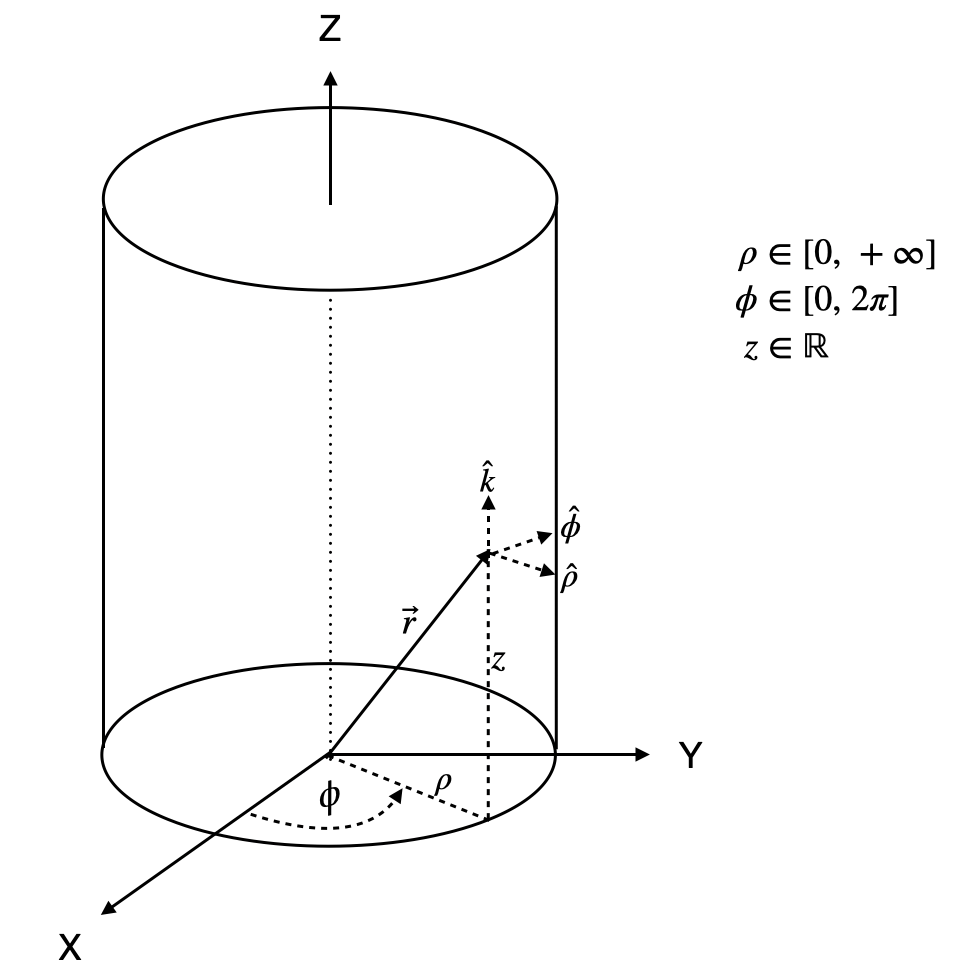
\includegraphics[width=0.45\textwidth]{Resultados Útiles/imgs/coords_cilind_DFI.png}
    \caption{Coordenadas cilíndricas en el plano cartesiano}
    \label{fig:C.cilindricas}
\end{figure}

\begin{minipage}{0.55\textwidth}
\begin{equation}
\begin{split}
    &x = \rho\cos{\phi}\\
    &y = \rho\sin{\phi}\\
\end{split}
\nonumber
\end{equation}
\end{minipage}
\begin{minipage}{0.35\textwidth}
\begin{equation}
\begin{split}
    & \rho = \sqrt{x^2+y^2}\\
    & \phi = \arctan{\frac{y}{x}}\\
\end{split}
\nonumber
\end{equation}
\end{minipage}

\bigbreak
Factores escalares:
\begin{itemize}
    \item $h_\rho = 1$
    \item $h_\phi = \rho$
    \item $h_z = 1$
\end{itemize}

Vectores unitarios:

\begin{itemize}
    \item $\hat{\rho} = \cos{\phi}\,\hat{x}+\sin{\phi}\,\hat{y}$
    \item $\hat{\phi} = -\sin{\phi}\,\hat{x}+\cos{\phi}\,\hat{y}$
    \item $\hat{x}=
    \cos{\phi}\,\hat{\rho}-\sin{\phi}\,\hat{\phi}$
    \item $\hat{y}=
    \sin{\phi}\,\hat{\rho}+\cos{\phi}\,\hat{\phi}$
\end{itemize}

\medbreak

Gradiente:

\[\nabla F = \frac{\partial F}{\partial \rho}\hat{\rho} + \frac{1}{\rho}\frac{\partial F}{\partial \phi}\hat{\phi} + \frac{\partial F}{\partial z}\hat{z}\]

Divergencia:

\[\nabla \cdot \vec{F} = \frac{1}{\rho}\left(\frac{\partial(F_{\rho}\rho)}{\partial\rho}+\frac{\partial F_{\phi}}{\partial\phi}+\frac{\partial(F_{z}\rho)}{\partial z}\right)\]

Rotor:
% Elimine un rho que acompañaba a dF_phi/dphi
\[\nabla\times\vec{F} = \frac{1}{\rho}\left(\frac{\partial F_{z}}{\partial \phi}-\rho\frac{\partial F_{\phi}}{\partial z}\right)\hat{\rho} + \left(\frac{\partial F_{\rho}}{\partial z}-\frac{\partial F_{z}}{\partial \rho}\right)\hat{\phi} + \frac{1}{\rho}\left(\frac{\partial(F_{\phi}\rho)}{\partial \rho}-\frac{\partial F_{\rho}}{\partial \phi}\right)\hat{z}\]

\medbreak

Diferenciales:

\begin{itemize}
    \item Linea:
    \[d\vec{r} = d\rho\hat{\rho} + \rho d\phi\hat{\phi}+dz\hat{z}\]
    \item Superficie:
    \[d\vec{S} = \rho\,d\phi dz\hat{\rho}+d\rho dz\hat{\phi}+\rho\, d\rho d\phi\hat{z}\]
    \item Volumen:
    \[dV = \rho\,d\rho d\phi dz\]
\end{itemize}

\newpage
%%%%%%%%%%%%%%%%%%%%%%%%%%%%%%%%%%%%%%%%%%%%%%%%%%%%%%
\subsection{Esféricas}

\[\Vec{r}(r,\phi,\theta)\]

\begin{figure}[H]
    \centering
    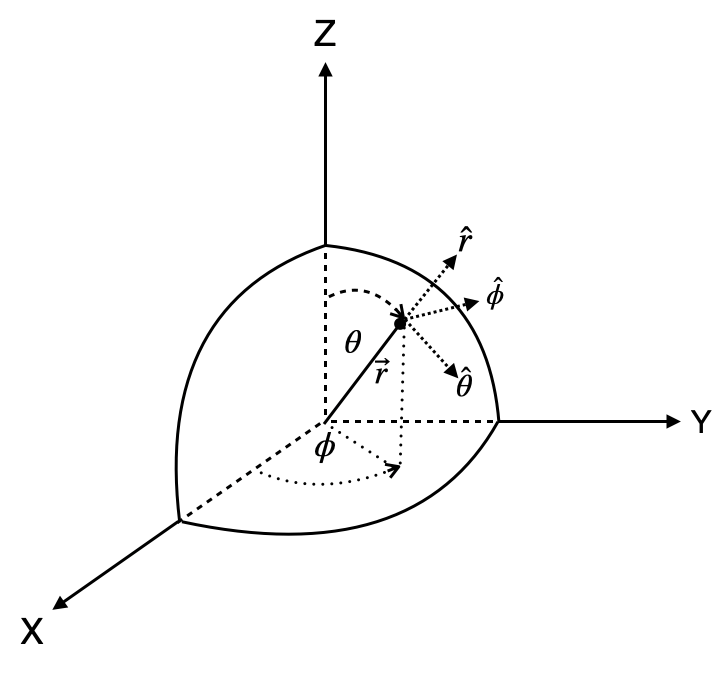
\includegraphics[width=0.5\textwidth]{Resultados Útiles/imgs/coords_esferc_DFI.png}
    \caption{Coordenadas esféricas en el plano cartesiano}
    \label{fig:C.esfericas}
\end{figure}

\begin{minipage}{0.55\textwidth}
\begin{equation}
\begin{split}
    &x = r\sin{\theta}\cos{\phi}\\
    &y = r\sin{\theta}\sin{\phi}\\
    &z = r\cos{\theta}\\
\end{split}
\nonumber
\end{equation}
\end{minipage}
\begin{minipage}{0.35\textwidth}
\begin{equation}
\begin{split}
    & r = \sqrt{x^2+y^2+z^2}\\
    & \phi = \arctan{\frac{y}{x}}\\
    & \theta = \arctan{\left(\frac{\sqrt{x^2+ y^2}}{z}\right)}
\end{split}
\nonumber
\end{equation}
\end{minipage}

\bigbreak
Factores escalares:
\begin{itemize}
    \item $h_r = 1$
    \item $h_\phi = r\sin{\theta}$
    \item $h_\theta = r$
\end{itemize}
\bigbreak
Vectores unitarios:

\begin{itemize}
    \item $\hat{r} = \sin(\theta)\cos(\phi)\hat{x} + \sin(\theta)\sin(\phi)\hat{y} + cos(\theta)\hat{z}$
    \item $\hat{\phi} = -\sin(\phi)\hat{x}+\cos(\phi)\hat{y}$
    \item $\hat{\theta} = \cos(\theta)cos(\phi)\hat{x} + \cos(\theta)\sin(\phi)\hat{y}-\sin(\theta)\hat{z}$
    \item $\hat{x}=\sin{(\theta)\cos{(\phi)}}\hat{r}-\sin{(\phi)}\hat{\phi}+\cos{(\theta)}\cos{(\phi)}\hat{\theta}$
    \item $\hat{y}=\sin{(\theta)\sin{(\phi)}}\hat{r}+\cos{(\phi)}\hat{\phi}+\cos{(\theta)}\sin{(\phi)}\hat{\theta}$
    \item $\hat{z}=\cos{(\theta)}\hat{r}-\sin{(\theta)}\hat{\theta}$
\end{itemize}

\bigbreak

Gradiente:

\[\nabla F = \frac{\partial F}{\partial r}\hat{r} + \frac{1}{rsin(\theta)}\frac{\partial F}{\partial \phi}\hat{\phi} + \frac{1}{r}\frac{\partial F}{\partial \theta}\hat{\theta}\]

Divergencia:

\[\nabla \cdot \vec{F} = \frac{1}{r^2sin(\theta)}\left(\frac{\partial(F_{r}r^2sin(\theta))}{\partial r}+\frac{\partial (F_{\phi}r)}{\partial\phi}+\frac{\partial(F_{\theta}rsin(\theta))}{\partial \theta}\right)\]

Rotor:

\[\nabla\times\vec{F} = \frac{1}{r\sin\theta} \left( \frac{\partial}{\partial \theta} \left(F_\phi\sin\theta \right) - \frac{\partial F_\theta}{\partial \phi} \right) \hat{r} + \frac{1}{r} \left( \frac{1}{\sin\theta} \frac{\partial F_r}{\partial \phi} - \frac{\partial}{\partial r} \left( r F_\phi \right) \right) \hat{\theta} + \frac{1}{r} \left( \frac{\partial}{\partial r} \left( r F_{\theta} \right) - \frac{\partial F_r}{\partial \theta} \right) \hat{\phi}\]

Diferenciales:

\begin{itemize}
    \item Linea:
    \[d\vec{r} = dr\hat{r} + r\sin(\theta)\, d\phi\hat{\phi}+r\,d\theta\hat{\theta}\]
    \item Superficie:
    \[d\vec{S} = r^2\sin(\theta)\,d\phi d\theta\hat{r}+r\,drd\theta\hat{\phi}+r\sin(\theta)\,dr d\phi\hat{\theta}\]
    \item Volumen:
    \[dV = r^2\sin(\theta)\,dr d\phi d\theta\]
\end{itemize}

\newpage
%%%%%%%%%%%%%%%%%%%%%%%%%%%%%%%%%%%%%%%%%%%%%%%%%%%%%%%%%%%%%
\subsection{Parabólicas}

\[\Vec{r}(\epsilon,\eta,\phi)\]

\begin{minipage}{0.55\textwidth}
\begin{equation}
\begin{split}
    &x = \epsilon\eta\cos{\phi}\\
    &y = \epsilon\eta\sin{\phi}\\
    &z = \frac{1}{2}(\eta^2-\epsilon^2)\\
\end{split}
\nonumber
\end{equation}
\end{minipage}
\begin{minipage}{0.35\textwidth}
\begin{equation}
\begin{split}
    & \epsilon = \sqrt{x^2+y^2+z^2}-z\\
    & \eta = \sqrt{x^2+y^2+z^2}+z\\
    & \phi = \arctan{\left(\frac{y}{x}\right)}
\end{split}
\nonumber
\end{equation}
\end{minipage}

\bigbreak
Factores escalares:
\begin{itemize}
    \item $h_\epsilon = \sqrt{\epsilon^2+\eta^2}$
    \item $h_\eta = \sqrt{\epsilon^2+\eta^2}$
    \item $h_\phi = \epsilon\eta$
\end{itemize}
\bigbreak
Vectores unitarios:

\begin{itemize}
    \item $\hat{\epsilon} = \frac{1}{\sqrt{\epsilon^2+\eta^2}}(\eta(\cos{\phi}\,\hat{x}+\sin{\phi}\,\hat{y})-\epsilon\hat{z})$
    \item $\hat{\eta} =  \frac{1}{\sqrt{\epsilon^2+\eta^2}}(\epsilon(\cos{\phi}\,\hat{x}+\sin{\phi}\,\hat{y})+\eta\hat{z})$
    \item $\hat{\phi} = -\sin{\phi}\,\hat{x}+\cos{\phi}\,\hat{y}$
\end{itemize}

\bigbreak

Gradiente:

\[\nabla F = \frac{1}{\sqrt{\epsilon^2+\eta^2}}\frac{\partial
 f}{\partial \epsilon}\hat{\epsilon}+\frac{1}{\sqrt{\epsilon^2+\eta^2}}\frac{\partial
 f}{\partial \eta}\hat{\eta}+\frac{1}{\epsilon\eta}\frac{\partial f}{\partial \phi}\hat{\phi}\]

Divergencia:

\[\nabla \cdot \vec{F} = \frac{1}{\epsilon\eta(\epsilon^2+\eta^2)}
\left(
\frac{\partial(F_\epsilon\epsilon\eta\sqrt{\epsilon^2+\eta^2})}{\partial\epsilon}+
\frac{\partial(F_\eta\epsilon\eta\sqrt{\epsilon^2+\eta^2})}{\partial\eta}+(\epsilon^2+\eta^2)
\frac{\partial F_\phi}{\partial\phi}\right)\]

Rotor:

\[\left(\nabla\times\vec{F}\right)_\epsilon =
\frac{1}{\epsilon\eta\sqrt{\epsilon^2+\eta^2}}
\left(\epsilon
\frac{\partial(F_\phi\eta)}{\partial\eta}-\sqrt{\epsilon^2+\eta^2}\frac{\partial F_\eta}{\partial\phi}\right)\]
\[\left(\nabla\times\vec{F}\right)_\eta=\frac{1}{\epsilon\eta\sqrt{\epsilon^2+\eta^2}}
\left(\sqrt{\epsilon^2+\eta^2}
\frac{\partial F_\epsilon}{\partial\phi}-\eta
\frac{\partial(F_\phi\epsilon)}{\partial\epsilon}\right)\]
\[\left(\nabla\times\vec{F}\right)_\phi=
\frac{1}{\epsilon^2+\eta^2}
\left(\frac{\partial(F_\eta\sqrt{\epsilon^2+\eta^2})}{\partial\epsilon}-\frac{\partial(F_\epsilon\sqrt{\epsilon^2+\eta^2})}{\partial\eta}\right)\]
\newpage
Diferenciales:

\begin{itemize}
    \item Linea:
    \[d\vec{r} = \sqrt{\epsilon^2+\eta^2}d\epsilon\,\hat{\epsilon} + \sqrt{\epsilon^2+\eta^2}d\eta\,\hat{\eta}+\epsilon\eta d\phi\,\hat{\phi}\]
    \item Superficie:
    \[d\vec{S} = \epsilon\eta\sqrt{\epsilon^2+\eta^2}\,d\eta d\phi\hat{\epsilon}+\epsilon\eta\sqrt{\epsilon^2+\eta^2}\,d\phi d\epsilon\hat{\eta}+(\epsilon^2+\eta^2)\,d\epsilon d\eta\hat{\phi}\]
    \item Volumen:
    \[dV = \epsilon\eta(\epsilon^2+\eta^2)\,d\epsilon d\eta d\phi\]
\end{itemize}

\subsection{Elípticas 1}

\[\Vec{r}(\mu,\theta,z)\]

\begin{minipage}{0.55\textwidth}
\begin{equation}
    x = a\cosh{\mu}\cos{\theta}\,\,\,\,\,\,\,\,
    y = a\sinh{\mu}\sin{\theta}
\nonumber
\end{equation}
\end{minipage}

\bigbreak
Factores escalares:
\begin{itemize}
    \item $h_\mu = a\sqrt{\cosh^2{\mu}\cos^2{\theta}
    +\sinh^2{\mu}\sin^2{\theta}}$
    \item $h_\theta = a\sqrt{\cosh^2{\mu}\cos^2{\theta}
    +\sinh^2{\mu}\sin^2{\theta}}$
\end{itemize}
\bigbreak
Vectores unitarios:

\begin{itemize}
    \item $\hat{\mu}=\frac{\sinh{\mu}\cos{\theta}\hat{x}+\cosh{\mu}\sin{\theta}\hat{y}}{\sqrt{\cosh^2{\mu}\cos^2{\theta}
    +\sinh^2{\mu}\sin^2{\theta}}}$
    \item $\hat{\theta}=\frac{-\cosh{\mu}\sin{\theta}\hat{x}+\sinh{\mu}\cos{\theta}\hat{y}}{\sqrt{\cosh^2{\mu}\cos^2{\theta}+\sinh^2{\mu}\sin^2{\theta}}}$
\end{itemize}

\bigbreak

%Gradiente:



%Divergencia:



%Rotor:



%Diferenciales:

%\begin{itemize}
%    \item Linea:
    
%    \item Superficie:
    
%    \item Volumen:
    
%\end{itemize}

\newpage
\section{Tabla Primitivas}
\textit{Se ignora la constante de integración para facilitar la visualización.}

\begin{minipage}{0.55\textwidth}
\begin{equation}
\begin{split}
    &\int\frac{1}{x}dx  = \ln{|x|} \\
    &\int e^{f(x)}f'(x)dx  = e^{f(x)} \\
    &\int \ln{x}dx  = x\ln{x}-x \\
    &\int x\ln{x}dx  = \frac{1}{4}x^2(2\ln{x}-1) \\
    &\int\frac{1}{x^2+a^2}\,dx  = \frac{1}{a}\arctan{\frac{1}{a}}\\
    &\int\frac{1}{\sqrt{x^2-a^2}}\,dx  = \sinh^{-1}{\frac{x}{a}}\\
    &\int\frac{1}{\sqrt{a^2-x^2}}\,dx  = \arcsin{\frac{x}{a}}\\
    &\int \frac{1}{\sqrt{x^2+a^2}}\,dx  = \cosh^{-1}{\frac{x}{a}}\\
    &\int\frac{1}{x\sqrt{x^2-a^2}}\,dx  = \frac{1}{a}\arctan{\left(\frac{\sqrt{x^2-a^2}}{a}\right)}\\
    &\int\frac{1}{x\sqrt{x^2+a^2}}\,dx  = -\frac{1}{a}\ln{\left(\frac{
    a+\sqrt{x^2+a^2}}{x}\right)}\\
    &\int\frac{1}{x\sqrt{a^2-x^2}}\,dx  = -\frac{1}{a}\ln{\left(\frac{a+\sqrt{a^2-x^2}}{x}\right)}\\
    &\int\frac{1}{x^2-a^2}\,dx  = \frac{\ln{|x-a|}-\ln{|x+a|}}{2a}\\
    &\int\frac{1}{a^2-x^2}\,dx  = \frac{\ln{|x+a|}-\ln{|x-a|}}{2a}\\
    &\int\frac{1}{(1+x^2)^2}\,dx  = \frac{x}{2(1+x^2)}+\frac{1}{2}\arctan{x}\\
    &\int|x|\,dx  = \frac{x\abs{x}}{2}\\
    &\int \sin^3{x}\,dx = \frac{1}{4}\left(\frac{\cos{3x}}{3}-3\cos{x}\right)\\
    &\int \cos^3{x}\,dx = \frac{1}{4}\left(\frac{\sin{3x}}{3}+3\sin{x}\right)\\
    %cabe 1 más
\end{split}
\nonumber
\end{equation}
\end{minipage}
\begin{minipage}{0.55\textwidth}
\begin{equation}
\begin{split}
    &\int \sin{x}\,dx = -\cos{x} \\
    &\int \cos{x}\,dx = \sin{x} \\
    &\int\tan{x}\,dx  = -\ln{|\cos{x}|} \\
    &\int\sec{x}\,dx  = \ln{|\sec{x}+\tan{x}|}\\
    &\int\csc{x}\,dx  = \ln{|\csc{x}-\cot{x}|}\\
    &\int\tan^2{x}\,dx  = \tan{x}-x \\
    &\int\cot^2{x}\,dx  = -\cot{x}-x \\
    &\int\cos^2{(ax)}\,dx  = \frac{x}{2}+\frac{\sin{(2ax)}}{4a}\\
    &\int\sin^2{(ax)}\,dx  = \frac{x}{2}-\frac{\sin{(2ax)}}{4a}\\
    &\int\cosh^2{(ax)}\,dx  = \frac{x}{2}+\frac{\sinh{(2ax)}}{4a}\\
    &\int\sinh^2{(ax)}\,dx  = \frac{\sinh{(2ax)}}{4a}-\frac{x}{2}\\
    &\int\frac{1}{\cosh{x}}\,dx  = 2\arctan{e^x}\\
    &\int\frac{1}{\sinh{x}}\,dx  = \ln{|e^x-1|}-\ln{|e^x+1|}\\
    &\int\sqrt{a^2-x^2}\,dx  = \frac{x}{2}\sqrt{a^2-x^2}+\frac{a^2}{2}\arcsin{\frac{x}{a}}\\
    &\int\sqrt{a^2+x^2}\,dx = \frac{x}{2}\sqrt{x^2+a^2}+\frac{a^2}{2}\ln{(x~\sqrt{x^2+a^2})}\\
    &\int\sqrt{x^2-a^2}\,dx = \frac{x}{2}\sqrt{x^2-a^2}-\frac{a^2}{2}\ln{(x+\sqrt{x^2-a^2})}\\
    &\int\frac{1}{(a^2+(b-x)^2)^{3/2}}\,dx=\frac{x-b}{a\sqrt{a^2+(b-x)^2}}\\
    %caben 1 ó 2 más
\end{split}
\nonumber
\end{equation}
\end{minipage}
\newpage
\begin{equation}
    \begin{split}
    &\int\frac{x}{\sqrt{a-bx}}\,dx= \frac{-2a}{b^2}\sqrt{a-bx}+\frac{2}{3b^2}(a-bx)^{3/2}\\
    &\int\frac{x}{\sqrt{ax^2 + bx +c}}\,dx = \frac{1}{a}\sqrt{ax^2 +bx +c} - \frac{b}{2a^{3/2}}\ln{\abs{2ax +b+2\sqrt{a(ax^2+bx+c)}}}\\
    &\int\frac{x}{(x^2+a^2)^{3/2}}\,dx = -\frac{1}{\sqrt{x^2 + a^2}} \quad \text{(Común en Electromagnetismo)}
    \end{split}
    \nonumber
\end{equation}
Para funciones de forma $\frac{Ax+B}{ax^2+bx+c}$, se tiene que:

\begin{itemize}
    \item Si $4ac>b^2$
    \[\int\frac{Ax+B}{ax^2+bx+c}\,dx = \frac{A}{2a}\ln{(ax^2+bx+c)}+\frac{2aB-bA}{a\sqrt{4ac-b^2}}\arctan{\left(\frac{2ax+b}{\sqrt{4ac-b^2}}\right)}\]
    \item Si $4ac<b^2$ %este puede que haya que revisarlo
    \[\int\frac{Ax+B}{ax^2+bx+c}\,dx = \frac{1}{2\sqrt{b^2-4ac}}
    \left(\Omega_{-}+\,\Omega_{+}\right)\]
    donde
    \[\Omega_{-} = (2B-A(b-\sqrt{b^2-4ac}))\ln{(2ax+b-\sqrt{b^2-4ac})}\]
    \[\Omega_{+} = (A(b+\sqrt{b^2-4ac})-2B)\ln{(2ax+b+\sqrt{b^2-4ac})}\]
\end{itemize}

\newpage
\section{Resultados Útiles}

En esta sección pondremos demostraciones que son necesarias o útiles para resolver varios problemas.

\subsection{Argumentos de simetría del campo eléctrico}

Para todas las demostraciones de simetría es necesario tener una distribución uniforme de carga e indicar, inicialmente al menos, de manera gráfica por que existe la simetría. Para cada demostración se hará uso de las coordenadas con la que es más fácil trabajar las figuras, pero aplica para todas las coordenadas haciendo las transformaciones pertinentes.

\subsubsection{En esferas}

\label{SimetríaEsfera}
En esferas el campo eléctrico tiene componente solo en $\hat{r}$ a causa de que los campos generados por cargas cercanas se cancelan entre sí, permitiendo solo la existencia en esa dirección. 

En la figura inferior se observa que los campos $\Vec{E}_2$ y $\Vec{E}_1$ generados por $\Delta q_1$ y $\Delta q_2$ en la dirección $P$ se cancelan entre sí, causando el campo $\Vec{E}_{neto}$ en la dirección radial a $P$.
\begin{figure}[H]
    \centering
    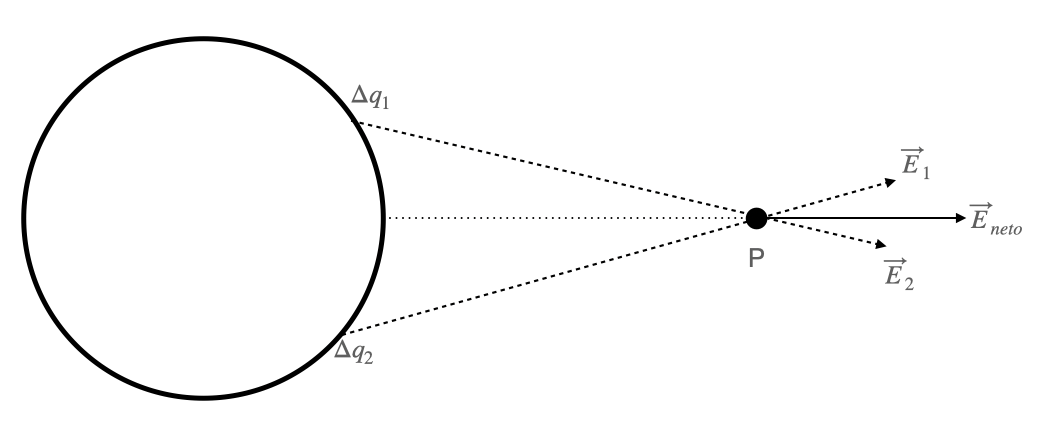
\includegraphics[width=0.7\textwidth]{Resultados utiles/demost_simetria_esfera.png}
    \label{fig:simetria_esfera}
\end{figure}

\subsubsection{En cilindros infinitos o con altura $\gg$ radio}

\label{SimetríaCilindrosInf}
En cilindros tales que sean de largo infinito o su largo sea mucho mayor ($\gg$) al radio, el campo eléctrico apuntará en la dirección $\hat{\rho}$, esto a que las componentes de los campos en $\hat{z}$ se cancelan entre sí.

En la figura inferior se observa esto, donde en el punto $P$ los campos $\Vec{E}_1$ y $\Vec{E}_2$ generados por $\Delta q_1$ y $\Delta q_2$ se cancelan entre sí dando origen al campo $\Vec{E}_{neto}$ en $\hat{\rho}$.
\begin{figure}[H]
    \centering
    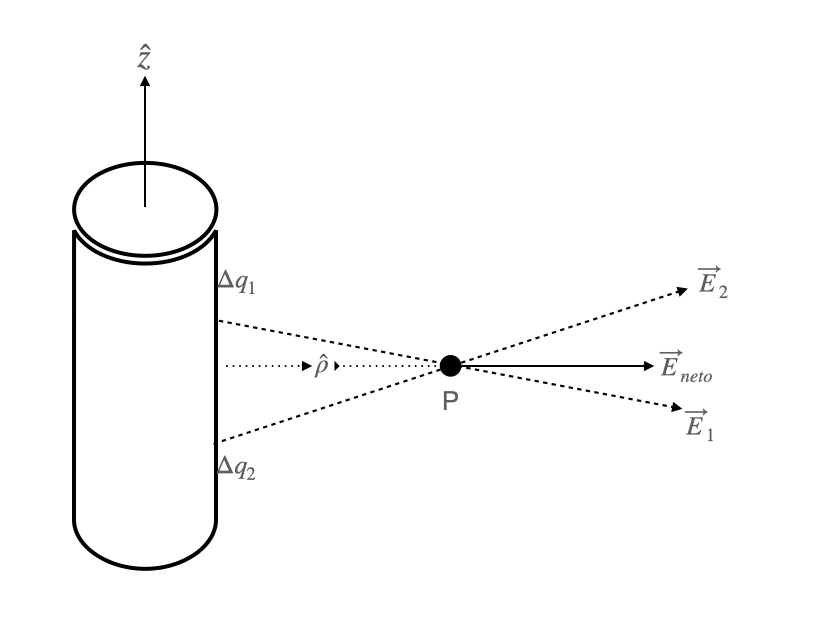
\includegraphics[width=0.7\textwidth]{Resultados utiles/demost_simetria_cili.png}
    \label{fig:simetria_cilindro}
\end{figure}
\subsubsection{En planos infinitos}
\label{SimetríaPlanosInf}
En planos infinitos o con largo 'muy grande', se tendrá que el campo solo apuntará en la dirección normal a la superficie, esto es a causa de que las componentes en las otras direcciones se cancelan entre sí. 
\medbreak
En la figura inferior se observa esto, donde la normal es $\hat{z}$.
\begin{figure}[H]
    \centering
    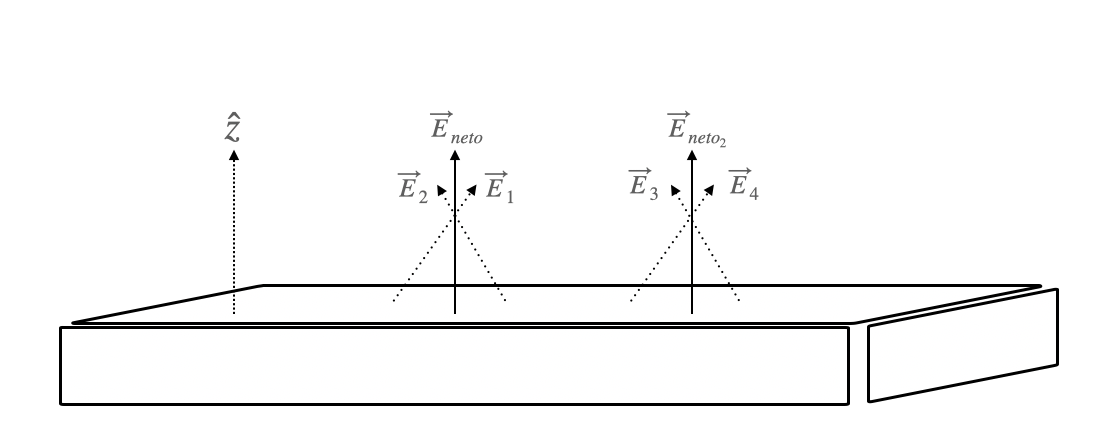
\includegraphics[width=0.7\textwidth]{Resultados utiles/demost_simetria_plano.png}
    \label{fig:simetria_plano}
\end{figure}
\medbreak
Tomando un punto $r$ arbitrario fuera del plano en el lado donde $z$ es positivo, para todo punto $p$ en el plano, existe $p'$ simétrico a $p$ respecto a la recta perpendicular al plano que pasa por $r$, tal que la suma de los vectores que apuntan de $p$ a $r$ y de $p'$ a $r$ es paralela al eje $z$

\[\Vec{pr} = \Vec{r}-\Vec{p} = (r_x-p_x)\hat{x} + (r_y-p_y)\hat{y} + r_z\hat{z}\]
\[\Vec{p'r} = \Vec{r}-\Vec{p'} = (p_x-r_x)\hat{x} + (p_y-r_y)\hat{y} + r_z\hat{z}\]
\[\Vec{pr}+\Vec{p'r} = 2r_z\hat{z}\]

Con esto, el campo eléctrico en el lado positivo de $z$ depende sólo de $z$

\[\Vec{E_p}(\Vec{z})=E_p(z)\hat{z}\]

El razonamiento es el mismo para el lado negativo de z, con la única diferencia que el campo apunta en sentido opuesto.

\subsection{Ecuación de Poisson para esferas}
\label{PoissonEsferas}
Por simetría el potencial de una esfera depende sólo de la componente $r$ de las coordenadas esféricas.


\[\nabla^2V =
\nabla\cdot\left(\frac{\partial V}{\partial r}\hat{r}\right) =
\frac{1}{r^2}\frac{\partial}{\partial r}\left(\frac{\partial V}{\partial r}r^2\right) =
\frac{\partial^2 V}{\partial r^2}+\frac{2}{r}\frac{\partial V}{\partial r}
\]
\begin{equation}
\begin{split}
\nabla^2V = -\frac{\rho}{\epsilon_o} & \Leftrightarrow
\frac{\partial}{\partial r}\left(\frac{\partial V}{\partial r}r^2\right) = -\frac{\rho r^2}{\epsilon_o}
\\
& \Leftrightarrow \frac{\partial V}{\partial r}r^2 =
-\frac{\rho}{\epsilon_o}\int r^2\,dr
\\
& \Leftrightarrow \frac{\partial V}{\partial r} =
\frac{A}{r^2} - \frac{\rho r}{3\epsilon_o}
\\
& \Leftrightarrow V =
\int\frac{A}{r^2} - \frac{\rho r}{3\epsilon_o}\,dr
\\
& \Leftrightarrow V = 
B-\frac{A}{r} - \frac{\rho r^2}{6\epsilon_o}
\\
\end{split}
\nonumber
\end{equation}

\subsection{Ecuación de Poisson para cilindros infinitos}
\label{PoissonCilindrosInf}
Por simetría el potencial de una cilindro infinito depende sólo de la componente $\rho$ de las coordenadas cilíndricas, la cual notaremos como $r$ para distinguirla de la densidad de carga volumétrica.

\[\nabla^2V =
\nabla\cdot\left(\frac{\partial V}{\partial r}\hat{r}\right) =
\frac{1}{r}\frac{\partial}{\partial r}\left(\frac{\partial V}{\partial r}r\right) =
\frac{\partial^2 V}{\partial r^2}+\frac{1}{r}\frac{\partial V}{\partial r}
\]

\begin{equation}
\begin{split}
\nabla^2V = -\frac{\rho}{\epsilon_o} & \Leftrightarrow
\frac{\partial}{\partial r}\left(\frac{\partial V}{\partial r}r\right) = -\frac{\rho r}{\epsilon_o}
\\
& \Leftrightarrow \frac{\partial V}{\partial r}r =
-\frac{\rho}{\epsilon_o}\int r\,dr
\\
& \Leftrightarrow \frac{\partial V}{\partial r} =
\frac{A}{r} - \frac{\rho r}{2\epsilon_o}
\\
& \Leftrightarrow V =
\int\frac{A}{r} - \frac{\rho r}{2\epsilon_o}\,dr
\\
& \Leftrightarrow V = 
A\ln{r} - \frac{\rho r^2}{4\epsilon_o} + B
\\
\end{split}
\nonumber
\end{equation}

\subsection{Capacitancia de placas cercanas}
\label{C:placas}
Para el caso de un condensador conformado por 2 placas geométricamente idénticas de área $A$ separadas por una distancia $d$, si $d$ es mucho menor a las dimensiones de las placas se puede aproximar el campo eléctrico al de una placa infinita (2 planos infinitos), este está dado por

\[\Vec{E}=\frac{\sigma}{\epsilon_o}\]

donde $\sigma$ es la densidad de carga de una de las placas. De la relación\newline $\Vec{E}=-\nabla V$ se desprende que el potencial entre las placas es

\[V(z) = -\frac{\sigma z}{\epsilon_o}+B\]

con $B$ una constante. La diferencia de potencial del condensador es

\[\Delta V=V(0)-V(d)=B-
\left(-\frac{\sigma d}{\epsilon_o}+B\right) =
\frac{\sigma d}{\epsilon_o}\]

finalmente, se obtiene la capacitancia como

\[C=\frac{Q}{\Delta V}=\frac{\epsilon_o}{\sigma d}\sigma A=
\frac{\epsilon_o A}{d}\]

\subsection{Índice de Soluciones}

\begin{itemize}
    \item $\Vec{E}$ de un plano infinito: \hyperlink{S.4.2}{\textbf{S.4.2}} c)
    \item $U_e$ de un cascarón esférico: \hyperlink{S.6.1}{\textbf{S.6.1}}
    \item Fuerza, torque y energía en relación al momento dipolar: \hyperlink{S.8.1}{\textbf{S.8.1}}
\end{itemize}

\newpage

%Campo eléctrico
\section{Campo Eléctrico}

Dada una carga puntual $q$ ubicada en $\Vec{r_q}$, se define en campo eléctrico que esta ejerce sobre un punto $\Vec{r}$ como

\[\Vec{E}(\Vec{r}) = \frac{q}{4\pi\epsilon_o}\frac{\Vec{r}-\Vec{r_q}}{\parallel\Vec{r}-\Vec{r_q}\parallel^3}\]

\subsection{Ecuaciones de Maxwell}

Las dos primeras ecuaciones de Maxwell en electrostática son

\begin{equation}
\begin{split}
    &\nabla\cdot\Vec{E}=\frac{\rho}{\epsilon_o}\\
    &\nabla\times\Vec{E}=0
\end{split}
\nonumber
\end{equation}
\bigbreak
La forma integral de la segunda ecuación es
\[\oint_{\Gamma}\Vec{E}\cdot d\Vec{l} = 0\]
\bigbreak
La forma integral de la primera ecuación es la ley de Gauss.

\subsection{Principio de Superposición}

El campo eléctrico es aditivo, es decir, el campo que ejercen $n$ cargas sobre un mismo punto está dado por

\[\Vec{E}(\Vec{r}) = \sum^n_{i=1}\Vec{E_i} = \sum^n_{i=1}\frac{q_i}{4\pi\epsilon_o}\frac{\Vec{r}-\Vec{r_i}}{\parallel\Vec{r}-\Vec{r_i}\parallel^3}\]
\bigbreak
En el caso de una distribución continua se tiene

\[\Vec{E}(\Vec{r}) = \frac{q}{4\pi\epsilon_o}\int\frac{\Vec{r}-\Vec{r_q}}{\parallel\Vec{r}-\Vec{r_q}\parallel^3}\,dq(\Vec{r_q})\]
\bigbreak
donde $dq(\Vec{r_q})$ puede ser $\lambda dr$, $\sigma dS$ o $\rho dV$, con $\lambda$ la densidad de carga lineal, $\sigma$ la densidad superficial y $\rho$ la densidad volumétrica.

\subsection{Ley de Coulomb}

Una carga $q$ que siente un campo eléctrico $\Vec{E}$ se ve sujeta a una fuerza eléctrica, que está dada por

\[\Vec{F} = q\Vec{E}\]

Por acción y reacción, la fuerza que ejerce $q$ sobre la fuente del campo es $\Vec{F} = -q\Vec{E}$.

\subsection{Ley de Gauss}

Se dice que una superficie $\Lambda$ es cerrada si esta encierra un volumen (el cual puede ser infinito). Si la carga total en el espacio encerrado por $\Lambda$ es $Q$, la ley de Gauss garantiza que se satisface la igualdad

\[\oint_{\Lambda} \Vec{E}\cdot d\Vec{S} = \frac{Q}{\epsilon_o}\]

Donde $\Vec{E}$ es el campo eléctrico generado por $Q$, en esta integral en específico se está evaluando en la superficie. Esta es la forma integral de la primera ecuación de Maxwell. El círculo en la integral sólo indica que $\Lambda$ es cerrada, de por sí no altera el cálculo.\\

La ley de Gauss permite determinar el valor del campo eléctrico si este presenta simetría, es decir, cumple que $\Vec{E}(\Vec{r}) = E(n)\hat{n}$, con $\Vec{n} = n\hat{n}$ un vector normal a la superficie. En este caso se verifica que

\[\frac{Q}{\epsilon_o} = \oint_{\Lambda} \Vec{E}\cdot d\Vec{S} = \int_{\Lambda} E(n)\hat{n}\cdot dS\hat{n} = \int_{\Lambda} E(n) \,dS\]

Luego, tomando $\Lambda$ tal que $n$ sea constante, se tiene

\[\int_{\Lambda} E(n)\,dS = E(n)\int_{\Lambda}\,dS\]

De forma que, si el área de $\Lambda$ es $A$, el campo eléctrico en $\Lambda$ es

\[\Vec{E}(\Vec{r}) = \frac{Q}{A\epsilon_o}\hat{n}\]

Para determinar si existe simetría basta ver que, dado un punto $p$ arbitrario en el espacio, la suma de todos vectores que conectan los puntos de la superficie a $p$ resulta perpendicular a la misma.
\bigbreak
La simetría se cumple en esferas, con $\hat{n}=\hat{r}$; cilindros de largo infinito, con $\hat{n}=\hat{\rho}$; y planos infinitos, con $\hat{n}=\hat{z}$. En los 3 casos se asume que el sistema de coordenadas es elegido acorde a la superficie.



\newpage
\subsection{Problemas}
--------------------------------------------------------
\\

\np
Dos varillas de longitud $L$ están a lo largo del eje $x$, una entre $x=a/2$ y $x=a/2+L$ y la otra entre $x=-a/2$ y $x=-a/2-L$. Cada varilla tiene carga positiva Q distribuida uniformemente.

\begin{enumerate}[label=\alph*)]
    \item Calcule el campo eléctrico producido por la segunda varilla en puntos a lo largo del eje $x$ positivo.
    \item Calcule la magnitud de la fuerza que ejerce una varilla sobre la otra.
\end{enumerate}

\np
\begin{enumerate}[label=\alph*)]
    \item Determine el campo eléctrico en todos los puntos del eje de un anillo de radio $R$ sobre el cual hay una densidad de carga uniforme $\lambda$.
    \item A partir de su resultado anterior, calcule el campo eléctrico creado por una corona circular de radios $R_1$ y $R_2$ ($R_1 < R_2$), sobre la cual hay una densidad de carga uniforme $\sigma$, en los puntos de su eje. Encuentre la magnitud y la dirección del campo eléctrico. Considere puntos arriba y abajo de la corona circular.
    \item ¿A qué se reduce su resultado si $R_1 \longrightarrow 0$? ¿Y si $R_2 \longrightarrow \infty$?
    \item Demuestre que en puntos sobre el eje de la corona (eje $z$) que estén suficientemente cerca del origen, la magnitud del campo eléctrico es aproximadamente proporcional a la distancia entre el centro de la corona circular y el punto. ¿Qué tan cerca es ”suficientemente cerca”?
\end{enumerate}

\np
\begin{enumerate}[label=\alph*)]
    \item Encuentre el campo eléctrico creado por un segmento rectilíneo de longitud $L$ dotado de una densidad de carga uniforme $\lambda$.
    \item A partir del resultado anterior, calcule el campo eléctrico en todos los puntos del espacio, producido por una línea infinita con densidad de carga $\lambda$.
    \item Calcule el flujo de campo eléctrico a través de una superficie cilíndrica cerrada, de largo h y radio R, concéntrica con la línea infinita.
    \item  Se tienen dos líneas infinitas con densidad de carga $\lambda$ y $-\lambda$, situadas a una distancia $2a$ una de la otra. Encuentre la fuerza por unidad de longitud que se establece entre los dos hilos. ¿Es atractiva o repulsiva?
\end{enumerate}
\newpage
\np
Considere un plano infinito (en las direcciones $x$ e $y$) de grosor $2R$ (en la dirección $z$), cargado con una densidad de carga volumétrica $\rho$ uniforme. Este plano tiene un agujero cilíndrico (cuyo eje coincide con el eje $y$) de radio $R$ sin cargas.
\begin{enumerate}[label=\alph*)]
    \item Determine el campo eléctrico en todo el espacio. Note que debería dividir el resultado en 3 zonas distintas.
    \item Calcule la fuerza que experimenta un alambre de largo $L$ con densidad de carga lineal uniforme $\lambda$ ubicado a una distancia $d$ del plano y extendido en la dirección $z$.
    \item Calcule la fuerza que experimenta un alambre de largo $L$ con densidad de carga lineal uniforme $\lambda$ ubicado a una distancia $d+L/2$ del plano y extendido en la dirección $y$.
\end{enumerate}

\begin{figure}[h]
    \centering
    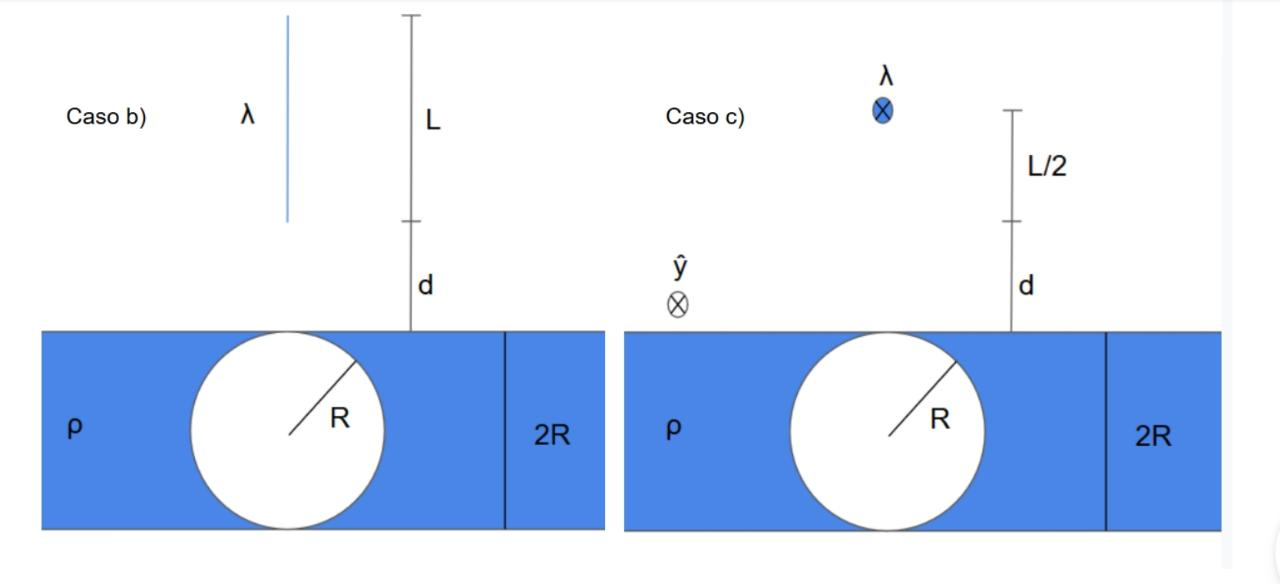
\includegraphics[width=0.9\textwidth]{Electroestática/Campo_electrico/P1 guia2 Mancilla.jpeg}
    \label{fig:P1G2M}
\end{figure}

\np
\begin{enumerate}[label=\alph*)]
    \item Si el campo eléctrico de una carga puntual fuera proporcional a $1/r^3$ en vez de $1/r^2$, ¿seguiría siendo válida la ley de Gauss? Explique su razonamiento. (Sugerencia: considere una superficie esférica centrada en una sola carga puntual).
    \item  Cierta región del espacio limitada por una superficie imaginaria cerrada no contiene carga. ¿El campo eléctrico siempre es igual a cero en todos los puntos de la superficie? Si no es así, ¿en qué circunstancias sería cero en la superficie?
    \item En cierta región del espacio, el campo eléctrico es uniforme. Use la ley de Gauss para demostrar que esa región debe ser eléctricamente neutra; es decir, la densidad volumétrica de carga $\rho$ debe ser igual a cero. Lo contrario, ¿es verdadero? Es decir, en una región del espacio donde no hay carga, ¿debe ser uniforme?
\end{enumerate}

\np
Imagine una esfera de radio R rellena con carga negativa de densidad uniforme y una carga total equivalente a la carga de dos electrones, es decir, $-2e$. En el interior de esta gelatina de carga negativa, se encuentran dos protones, cada uno de ellos de carga $e$. Asuma que, a pesar de la presencia de los protones, la distribución de carga negativa se mantiene uniforme. ¿Dónde deben ubicarse los protones de modo que la fuerza en cada uno de ellos sea nula? Para responder esta pregunta, siga estos pasos:
\begin{enumerate}[label=\alph*)]
    \item Calcule el campo eléctrico producido por los electrones.
    \item Calcule la fuerza de Coulomb neta sobre uno los protones.
    \item Determine la condición de equilibrio y concluya.
\end{enumerate}


\newpage
\subsection{Soluciones}

\sol{1}\newline\newline
$a)$ Al ser metálicas, la esfera y el cascarón son conductores.En equilibrio electrostático, la carga en la superficie interior del cascarón es $-q$ para neutralizar el campo eléctrico de la esfera (que no haya líneas de campo en el conductor) y, dado que su carga total es nula, la carga en la superficie exterior es $q$. Las densidades de carga superficial de la esfera $\sigma_S$, interior del cascarón $\sigma_I$ y exterior del cascarón $\sigma_E$ son uniformes, en el caso de $\sigma_I$ porque la esfera y el cascarón son concéntricos, y están dados por

\[\sigma_S = \frac{q}{4\pi R^2}\]
\[\sigma_I = \frac{-q}{4\pi a^2}\]
\[\sigma_E = \frac{q}{4\pi b^2}\]

$b)$ El espacio está dividido en 4 zonas: al interior de la esfera, $r<R$ (1); entre la esfera y el cascarón, $R<r<a$ (2); interior del cascarón, $a<r<b$ (3); y exterior del cascarón, $b<r$ (4). Como el sistema se compone sólo de conductores y vacío, la densidad volumétrica en todo el espacio es nula. Con esto, utilizando la ecuación de Poisson (calculada en \textbf{\ref{PoissonEsferas}}) el potencial dividido en zonas es

\begin{itemize}
    \item $V_1 = B_1 - \frac{A_1}{r}$
    \item $V_2 = B_2 - \frac{A_2}{r}$
    \item $V_3 = B_3 - \frac{A_3}{r}$
    \item $V_4 = B_4 - \frac{A_4}{r}$
\end{itemize}

Para $r\rightarrow\infty$ el potencial se anula, por lo que $B_4 = 0$, además, dado que en los conductores el potencial es constante, $A_1 = A_3 = 0$.

Los campos eléctricos en (2) y (4) poseen simetría de tipo $\Vec{E}(\Vec{r}) = E(r)\hat{r}$ (demostración en \textbf{\ref{SimetríaEsfera}}), de modo que por ley de Gauss se verifica que

\begin{itemize}
    \item $E_2 = \frac{q}{4\pi\epsilon_o r^2}$
    \item $E_4 = \frac{q}{4\pi\epsilon_o r^2}$
\end{itemize}

Utilizando $\Vec{E} = -\nabla V$ se obtiene

\[\frac{q}{4\pi\epsilon_o r^2} = -\frac{A_2}{r^2} = -\frac{A_4}{r^2}\]

\[A_2 = A_4 = -\frac{q}{4\pi\epsilon_o}\]

Finalmente, por continuidad del potencial

\[V_4(b) = V_3(b) \Rightarrow B_3 = \frac{q}{4\pi\epsilon_o b}\]
\[V_3(a) = V_2(a) \Rightarrow B_2 = \frac{q}{4\pi\epsilon_o}
\left(\frac{1}{b}-\frac{1}{a}\right)\]
\[V_2(R) = V_1(R) \Rightarrow B_1 = \frac{q}{4\pi\epsilon_o}
\left(1+\frac{1}{b}-\frac{1}{a}\right)\]

Se concluye así que

\begin{itemize}
    \item $V_1 = \frac{q}{4\pi\epsilon_o}
\left(1+\frac{1}{b}-\frac{1}{a}\right)$
    \item $V_2 = \frac{q}{4\pi\epsilon_o}\left(
    \frac{1}{r}+\frac{1}{b}-\frac{1}{a}\right)$
    \item $V_3 = \frac{q}{4\pi\epsilon_o b}$
    \item $V_4 = \frac{q}{4\pi\epsilon_o r}$
\end{itemize}
\bigbreak

$c)$ Si se baja el potencial del cascarón a 0, en consecuencia el potencial al exterior de este se anula también

\[V_3 = V_4(b) \Leftrightarrow 0 = -\frac{A_4}{b} \Leftrightarrow A_4 = 0	\Leftrightarrow V_4 = 0\]

Si $V_4 = 0$ entonces $E_4= 0$ y, por ley de Gauss, la carga total encerrada por el cascarón en nula, $\sigma_E = 0$. La carga de la esfera no se ve afectada, de modo que $E_2$ y $A_2$ se mantienen iguales, luego

\[V_2(a) = V_3 \Leftrightarrow B_2 = -\frac{q}{4\pi\epsilon_o a}\]
\[V_2(r) = \frac{q}{4\pi\epsilon_o}\left(\frac{1}{r}
-\frac{1}{a}\right)\]
\[V_1 = V_2(R) = \frac{q}{4\pi\epsilon_o}\left(\frac{1}{R}
-\frac{1}{a}\right)\]

\bigbreak

$d)$ Si $V_3 = V$ entonces

\[V_3 = V_4(b) \Leftrightarrow v = -\frac{A_4}{b} \Leftrightarrow A_4 = -Vb	\Leftrightarrow V_4 = \frac{Vb}{r}\]
\[V_2(a) = V_3 \Leftrightarrow B_2 = V-\frac{q}{4\pi\epsilon_o a}
\Leftrightarrow V_2 = V+\frac{q}{4\pi\epsilon_o}\left(\frac{1}{r}
-\frac{1}{a}\right)\]
\[\Vec{E_4}=-\nabla V_4 = \frac{Vb}{r^2}\hat{r}\]

Para $Q$ la carga total, por ley de Gauss se tiene que

\[E_4= \frac{Q}{4\pi\epsilon_o r^2} = \frac{Vb}{r^2}
\Leftrightarrow Q = 4\pi\epsilon_o Vb\]

Por lo que la carga neta del cascarón es

\[q_c = 4\pi\epsilon_o Vb - q\]

\bigbreak

$e)$ Si se conectan la esfera y el cascarón ambos conformarán un solo conductor y por lo tanto estarán a un mismo potencial. Como la diferencia de potencial es nula, el campo eléctrico en todo el espacio encerrado por el cascarón es 0. Dado que no se produce ningún cambio a la carga total, $E_4$, y por ende $V_4$, son los calculados en $b)$

\[V_1=V_2=V_3=V_4(b)=\frac{q}{4\pi\epsilon_o b}\]
\bigbreak

$f)$ La energía de los conductores desconectados es

\[U_{e1} = \frac{1}{2}(qV_1 + 0\cdot V_3) = \frac{q^2}{8\pi\epsilon_o}
\left(1+\frac{1}{b}-\frac{1}{a}\right)\]

Para los conductores conectados la energía es

\[U_{e2} = \frac{1}{2}qV_3 = \frac{q^2}{8\pi\epsilon_o b}\]

Se tiene $U_{e1} > U_{e2}$ debido a que al conectar los cascarones las cargas se desplazan a causa de un trabajo hecho por el campo, causando que la energía en el sistema disminuya.%para $U_{e1}$ a la energía de los conductores se le agrega la de la interacción entre ambos.

\bigbreak
\bigbreak

\sol{2}\newline\newline
Dado que $L \gg R_1, R_2$ el efecto que tiene cada esfera sobre el potencial de la otra puede ser despreciado. Para $q_1$ y $V_1$ la carga y potencial de la esfera de radio $R_1$, y $q_2$ y $V_2$ la carga y potencial de la esfera de radio $R_2$, se tiene

\[V_1 = \int\frac{\sigma_1}{4\pi\epsilon_o R_1}dS = 
\frac{q_1}{4\pi\epsilon_o R_1}\]

\[V_2 = \frac{q_2}{4\pi\epsilon_o R_2}\]

Como están conectadas, el potencial de las esferas debe ser igual

\[V_1 = V_2 \Leftrightarrow \frac{q_1}{R_1} = \frac{q_2}{R_2}\]

luego

\[Q = q_1 + q_2 = q_1 + \frac{R_2}{R_1}q_1 \Leftrightarrow
q_1 = \frac{R_1 Q}{R_1+R_2}\]

\[q_2 = \frac{R_2 Q}{R_1+R_2}\]

Puesto que $R_1<R_2$, la carga almacenada en la esfera de radio $R_2$ es mayor a la de radio $R_1$

\bigbreak

$b)$ El alambre es parte del conductor por lo que

\[V_{alambre} = V_1 = V_2 = \frac{Q}{4\pi\epsilon_o(R_2+R_1)}\]
\bigbreak

$c)$ La densidad de carga de las esferas es

\[\sigma_1 = \frac{q_1}{4\pi R_1^2} =
\frac{Q}{4\pi R_1(R_1+R_2)}\]
\[\sigma_2 = \frac{q_2}{4\pi R_2^2} =
\frac{Q}{4\pi R_2(R_1+R_2)}\]

Como $R_2 > R_1$, $\sigma_2 < \sigma_1$. El campo eléctrico en las superficies es

\[\Vec{E_1}=\frac{\sigma_1}{\epsilon_o}\hat{r_1}\]
\[\Vec{E_2}=\frac{\sigma_2}{\epsilon_o}\hat{r_2}\]

Donde $\hat{r_i}$ es el vector unitario $\hat{r}$ de las coordenadas esféricas respecto al centro de la esfera de radio $R_i$.
\bigbreak
\bigbreak

\sol{3}\newline\newline
 Usando coordenadas esféricas con origen en el centro de las capas, el espacio se divide en 4 zonas: $r < a$ (1), $a<r<2a$ (2), $2a<r<3a$ (3) y $3a<r$ (4). Las esferas presentan simetría (demostración en \textbf{\ref{SimetríaEsfera}}), por lo que se puede calcular su campo eléctrico con ley de Gauss. Como el sistema comprende sólo conductores y vacío $\rho = 0$ en todo el espacio. De la ecuación de Poisson (resuelta en \ref{PoissonEsferas}) se desprende que en cada zona el potencial es de forma
\[V = B-\frac{A}{r}\]


\begin{enumerate}[label=\alph*)]
    \item Como en (1) no hay carga el campo es nulo
    \[E_1 = 0\]
    \item En (2) la carga encerrada es $Q_{in}$, por lo que el campo eléctrico es
    \[\Vec{E_2} = \frac{Q_{in}}{4\pi\epsilon_o r^2}\hat{r}\]
    \item En (3) la carga encerrada es $Q_{in}+Q$, por lo que el campo eléctrico es
    \[\Vec{E_2} = \frac{Q_{in}+Q}{4\pi\epsilon_o r^2}\hat{r}\]
    \item Para que no haya campo eléctrico al interior del conductor exterior se debe cumplir que $Q_{out} = -(Q+Q_{in})$. Como en el infinito el potencial se anula, en (4) $B=0$ y $V = -\frac{A}{r}$. Igualando $V$ a 0 en $3a$ se obtiene que $A=V=0$ y en concecuencia
    \[E_4 = 0\]


    \item Para $V_2$ el potencial en (2), se verifica que

    \begin{equation}
    \begin{split}
        V_2(r) & = V_2(r) - V_2(a)\\
        & = -\int^r_a\Vec{E_2}\cdot d\Vec{r'}\\
       & = -\int^r_a\frac{Q_{in}}{4\pi\epsilon_o {r'}^2}\,dr'\\
       & = \frac{Q_{in}}{4\pi\epsilon_o r} - \frac{Q_{in}}{4\pi\epsilon_o a}\\
    \end{split}
    \nonumber
    \end{equation}
    Con lo que el potencial en la capa intermedia es

    \[V_2(2a) = -\frac{Q_{in}}{8\pi\epsilon_o a}\]
    \medbreak
    Para $V_3$ el potencial en (3), se verifica que

    \begin{equation}
    \begin{split}
      V_3(r) & = V_3(r) - V_3(3a)\\
      & = -\int^r_{3a}\Vec{E_3}\cdot d\Vec{r'}\\
      & = -\int^r_{3a}\frac{Q_{in}+Q}{4\pi\epsilon_o {r'}^2}\,dr'\\
      & = \frac{Q_{in}+Q}{4\pi\epsilon_o r} - \frac{Q_{in}+Q}{12\pi\epsilon_o a}\\
    \end{split}
    \nonumber
    \end{equation}
    Con lo que el potencial en la capa intermedia es

    \[V_3(2a) = \frac{Q_{in}+Q}{24\pi\epsilon_o a}\]
    \medbreak
    \item Como $V_2(2a)=V_3(2a)$, se tiene que

    \[\frac{Q_{in}+Q}{24\pi\epsilon_o a} = -\frac{Q_{in}}{8\pi\epsilon_o a}\]
    \[\implies Q_{in}=-\frac{1}{4}Q\]
    
    \medbreak
    \item Puesto que las capas exterior e interior están a igual potencial se las puede tomar como un solo conductor de carga $Q_{in} + Q_{out} = -Q$, formando un condensador con la capa intermedia. La capacitancia del sistema está dada por
    
    
    \[C = \frac{Q}{\Delta V} = 32\pi\epsilon_o a\]
    
    Esto también se puede ver como si se tuvieran dos condensadores en paralelo, uno con carga $Q_{in}$ y otro con carga $Q_{out}$ y misma diferencia de potencial $V(2a)$. Al estar en paralelos su capacitancia equivalente sería la suma de las capacitancias individuales, dando el resultado anterior.
    
    La razón de que pueden verse como condensadores en paralelo yace en que poseen el mismo potencial en ambos extremos, en uno están a potencial $V=0$ y en el otro a potencial $V = V(2a)$. En la siguiente imagen se visualiza de manera circuital
    
    \begin{figure}[H]
        \centering
        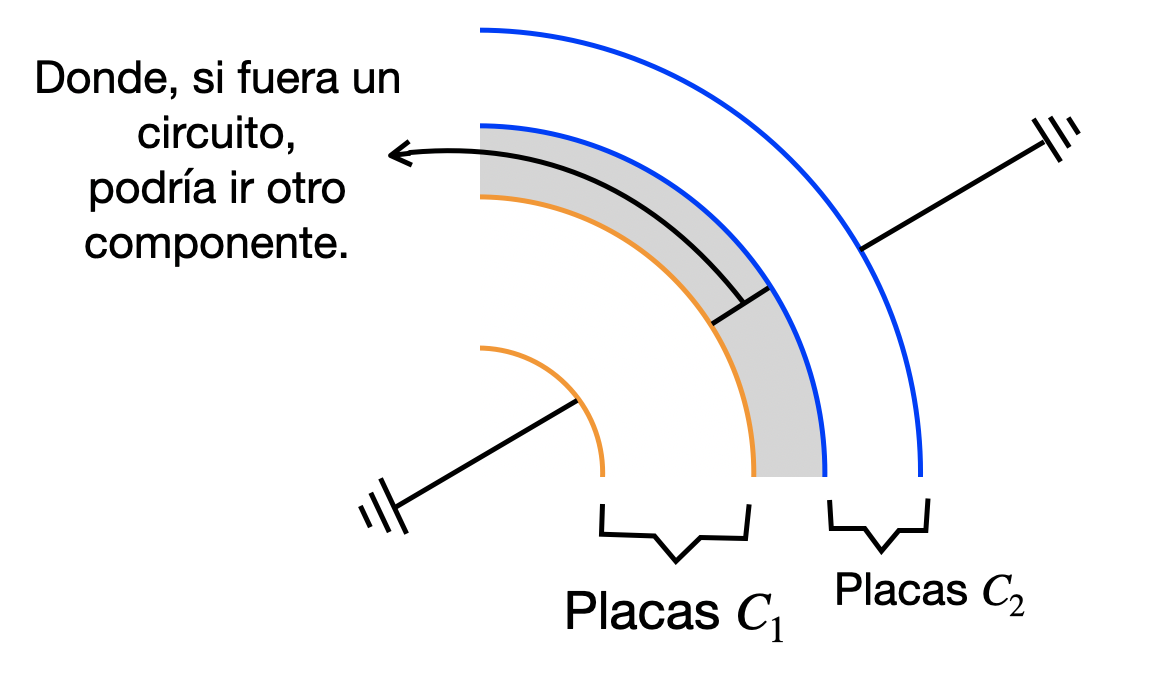
\includegraphics[width=0.5\textwidth]{Electroestática/conductores/P3IG.png}
    \end{figure}
    
    En la figura anterior el conductor de radio $a$ es el inferior izquierdo, el conductor de radio $2a$ está representado por el conductor 'con anchura' de color gris, y el conductor de radio $3a$ es el superior derecho. Las conexiones con 3 líneas representan conexiones a tierra. Y los condensadores son representados el primero con color amarillo-naranjo y el segundo con color azul. 
    
    \medbreak
    \item El sistema está compuesto por 3 conductores y 2 condensadores, como las capas interna y externa tienen potencial nulo, la energía queda dada sólo por la capa intermedia

    \[U_e = \frac{1}{2}V_2(2a) = \frac{1}{8}\frac{Q^2}{8\pi\epsilon_o a}\]
    
    Esto es equivalente a calcular la capacitancia de un condensador equivalente y, haciendo uso de $V(2a)$, obtener la energía potencial con
    $U_e = \frac{1}{2}C\Delta V^2$. 

\end{enumerate}
\bigbreak
\bigbreak
\sol{4}\newline
% Podriamos especificar la alineación de las placas y agregar imagen

\begin{enumerate}[label=\alph*)]
    %a
    \item Como las dimensiones laterales de las placas son mucho más grandes que $x$, se puede aproximar el campo eléctrico de una de las placas al de un plano infinito

    \[\Vec{E} = \frac{Q}{2A\epsilon_o}\hat{x}\]

    ubicando el origen en la placa de carga $Q$, el trabajo par desplazar la placa de carga $-Q$ en $\Delta x$ es

    \begin{equation}
        \begin{split}
            W_{ext} &= Q\int^{x+\Delta x}_x \Vec{E}\cdot d\Vec{r}\\
            & = Q\int^{x+\Delta x}_x\frac{Q}{2A\epsilon_o}\,dr\\
            & = \frac{Q^2}{2A\epsilon_o}\Delta x\\
        \end{split}
        \nonumber
    \end{equation}
    \medbreak
%b
    \item Por teorema de trabajo-energía, se cumple que la diferencia de energía potencial es igual al trabajo hecho por la fuerza externa, por lo que

    \[\Delta U_e = W = \frac{Q^2}{2A\epsilon_o}\Delta x\]
    Notemos que al ser el trabajo positivo, la fuerza externa está inyectando energía al sistema, por lo que se tiene que no se conserva la energía del sistema al aumentar la separación entre las placas por un $\Delta x$
    
    La energía potencial del sistema también se puede calcular haciendo uso del condensador, donde $U_e = \frac{1}{2}Q\Delta V = \frac{Q^2}{2C}$. Como se tiene que la carga de las placas no cambia, entonces se tiene que $C$ y $\Delta V$ han de cambiar. En específico, como se separan las placas $C$ pasa a ser $\frac{\epsilon_o A}{x+\Delta x}$ (calculado en \ref{C:placas}).
%c Aux_5 Daniela Mancilla Otoño 2020
    \item Siguiendo la idea del párrafo anterior, si es que al realizar trabajo cambia la energía del sistema, lo que implica un cambio en el condensador, (carga o diferencia de potencial) entonces al mantener la batería conectada se mantendrá la diferencia de potencial igual. Con esto en mente, entonces será necesario que la carga del condensador cambie.
    
    \begin{equation}
    \begin{split}
        W_{ext} &= \int^{x+\Delta x}_x Q\Vec{E}\cdot d\Vec{r}\\
        & = \int^{x+\Delta x}_x \frac{Q^2}{2A\epsilon_o}\,dr\\
        & = \int^{x+\Delta x}_x
        \frac{(CV_o)^2}{2A\epsilon_o}\,dr\\
        & = \int^{x+\Delta x}_x
        \frac{\epsilon_o AV_o^2}{2r^2}\,dr\\
        &=\frac{\epsilon_o AV_o^2}{2}\left(
        -\frac{1}{x+\Delta x}+\frac{1}{x}\right)\\
        &=\frac{\epsilon_o AV_o^2\Delta x}{2x(x+\Delta x)}
    \end{split}
    \nonumber
    \end{equation} 
    
    \medbreak

%d
    \item La energía potencial eléctrica inicial es
    
    \[U_i = \frac{1}{2}C_iV_o^2 = \frac{\epsilon_o A}{2x}V_o^2\]
    
    la energía potencial final es
    
    \[U_f = \frac{1}{2}C_fV_o^2 = 
    \frac{\epsilon_o A}{2(x+\Delta x)}V_o^2\]
    
    de modo que
    
    \[\Delta U = U_f-U_i = -\frac{\epsilon_o AV_o^2\Delta x}{2x(x+\Delta x)}\]
    
    % Hay que mostrar que la energía que se conserva

\end{enumerate}

\bigbreak
\bigbreak

\sol{5}\newline

\begin{enumerate}[label=\alph*)]
    \item El campo eléctrico en todo el espacio puede ser obtenido haciendo uso de la Ley de Gauss y de la definición de campo eléctrico, debido a lo que será pedido en los siguientes incisos solo será calculado en el caso $\rho > a$ y $\abs{z} < L/2$. Donde se están usando coordenadas cilíndricas y el centro del cilindro como eje.\\
    
    Partamos calculando la densidad superficial de carga, la densidad de carga es superficial a causa de que estamos frente a un conductor que no puede tener campo eléctrico interno, con esto tenemos que 
    \[\sigma = \frac{Q}{2\pi aL}\]
    A causa de que está solo en el manto y el área del manto es $2\pi aL$.\\
    
    Haciendo uso de la Ley de Gauss y sabiendo que por simetría (\ref{SimetríaCilindrosInf}) hay solo campo en la dirección $\hat{\rho}$, establecemos un cilindro más grande superpuesto con el original, de radio $\rho$ y altura $h$, con esto
    %no tiene que ser infinito?, no también el largo(altura) puede ser mucha mayor al radio
    \begin{equation}
        \begin{split}
            &\oint_{Manto} \Vec{E}\cdot d\Vec{S} = \frac{Q_{enc}}{\epsilon_0}\\
            \implies &\int E(\rho)dS = \frac{\sigma 2\pi a h}{\epsilon_0}\\
            \implies &E(\rho) \int dS = \frac{\sigma 2\pi a h}{\epsilon_0}\\
            \implies &E(\rho) 2 \pi \rho h = \frac{\sigma 2\pi a h}{\epsilon_0}\\
            \implies &E(\rho) = \frac{\sigma a}{\epsilon_0 \rho}\\
            \therefore \quad &\Vec{E}(\rho) = \frac{\sigma a}{\epsilon_0 \rho}\hat{\rho}
        \end{split}
        \nonumber 
    \end{equation}
    
    \item Sea $\sigma_+$ la densidad superficial del manto del cilindro de radio $a_1$ y $\sigma_-$ la densidad superficial del manto del cilindro de radio $a_2$, tenemos que el campo eléctrico de cada cilindro será
    
    \[\Vec{E}_{a_1} = \frac{\sigma_+ a_1}{\epsilon_0 \rho}\hat{\rho}\]
    \[\Vec{E}_{a_2} = \frac{\sigma_- a_2}{\epsilon_0 \rho}\hat{\rho'}\]
    
    Si calculamos el campo en $P$ debemos sumar ambos campos, y se tiene que $\hat{\rho'} = - \hat{\rho}$, ya que están centrados en distintos ejes los campos, y en $P$ las direcciones son justo contrarias, así
    
    \[\Vec{E}_{\text{en P}} = \left( \frac{\sigma_+ a_1}{\epsilon_0 r} - \frac{\sigma_- a_2}{\epsilon_0 (d-r)} \right)\hat{\rho}\]
    
    \item Para calcular la diferencia de potencial calculamos $V(a_1) - V(d - a_2)$ por definición,
    
    \begin{equation}
        \begin{split}
            V(a_1) - V(d - a_2) &= -\int_{d-a_2}^{a_1}\left[ \frac{\sigma_+ a_1}{\epsilon_0 r} - \frac{\sigma_- a_2}{\epsilon_0 (d-r)} \right]dr\\
            &= -\left.\left[ \frac{\sigma_+ a_1}{\epsilon_0}\ln{(r)} + \frac{\sigma_- a_2}{\epsilon_0}\ln{(d-r)} \right]\right\rvert_{d-a_2}^{a_1}\\
            &\vdots \quad\\ 
            &\approx -\left[ \frac{\sigma_+}{\epsilon_0}a_1\ln{\left( \frac{a_1}{d} \right)} - \frac{\sigma_-}{\epsilon_0}a_2\ln{\left( \frac{a_2}{d} \right)} \right]\\
            \text{Donde en } \vdots \text{ se usó que } &d-a_1 \approx d\text{ y } d-a_2 \approx d\text{, al ser }d \gg a_1\text{ y } d \gg a_2\\
        \end{split}
        \nonumber
    \end{equation}
    
    Reemplazamos $\sigma_+ = Q/(2\pi La_1)$ y $\sigma_- = -Q/(2\pi La_2)$, y nos queda
    
    \begin{equation}
        \begin{split}
            \Delta V &= -\left[ \frac{Q}{2 \pi L\epsilon_0}\ln{\left( \frac{a_1}{d} \right)} + \frac{Q}{2 \pi L\epsilon_0}\ln{\left( \frac{a_2}{d} \right)} \right]\\
            &=\frac{Q}{2 \pi L \epsilon_0}\ln{\left( \frac{d^2}{a_1a_2} \right)}\\
            &=\frac{Q}{\pi L \epsilon_0}\ln{\left( \frac{d}{\sqrt{a_1a_2}} \right)}
        \end{split}
        \nonumber
    \end{equation}
    
    Lo que nos da que la capacitancia del sistema es
    \[C_{tot} \approx \frac{Q}{\Delta V} = \frac{\pi \epsilon_0 L}{\ln{\left( \frac{d}{\sqrt{a_1a_2}} \right)}}\]
    
    \item Como se tiene que nos piden la capacitancia por unidad de largo debemos dividir la capacitancia encontrada por $L$, así
    \[C \approx \frac{\pi \epsilon_0}{\ln{\left( \frac{d}{\sqrt{a_1a_2}} \right)}}\]
    
    \item Está situación es similar a la presentada en el problema 7.2, por lo que las cargas se distribuirían a través de los cilindros dependiendo de las razones entre sus radios, y el potencial se volvería el mismo para ambos.
    
\end{enumerate}

\sol{6}\newline

\begin{enumerate}[label=\alph*)]
    \item Digamos que la capa del radio interno tiene una carga $-Q$ en su cara exterior, y la capa externa una carga $Q$ en su cara interior. Así queda la configuración como en la siguiente imagen
    \begin{figure}[H]
        \centering
        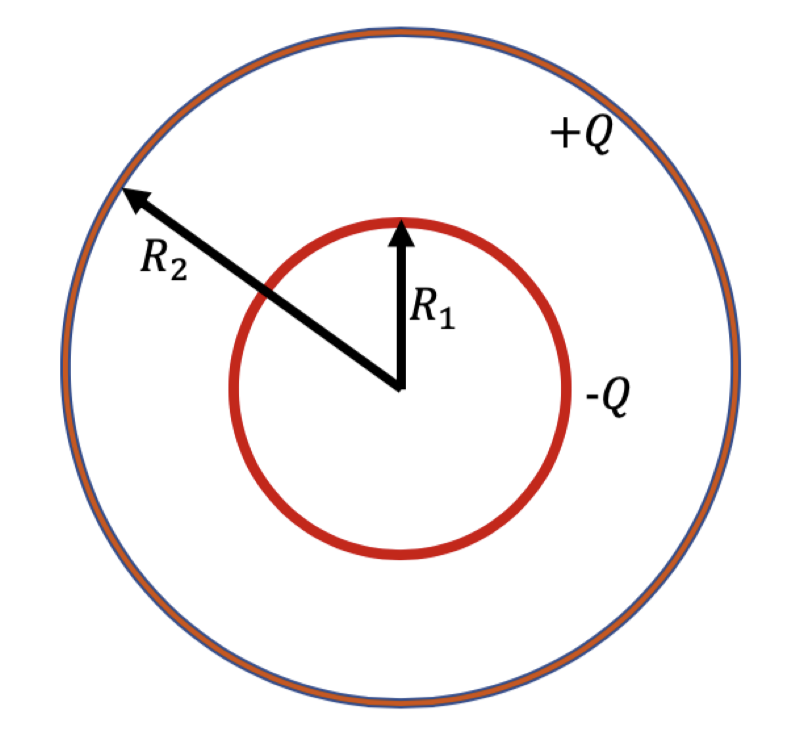
\includegraphics[width=0.47\textwidth]{Electroestática/conductores/P6IA.png}
        \label{fig:sol_6_conduc}
    \end{figure}
    
    Para calcular la capacitancia calculemos la diferencia de potencial entre ambas caras, para esto calculemos el campo eléctrico e integramos de $R_1$ a $R_2$.\\
    
    Usando Ley de Gauss y una superficie Gaussiana de largo $L$ y radio $\rho$, con $R_1 < \rho < R_2$,
    \[\oint_{Manto} \Vec{E}\cdot d\Vec{S} = \frac{Q_{enc}}{\epsilon_0}\]
    \[\implies E(\rho) = \frac{-Q}{2 \pi L \epsilon_0 \rho}\]
    Ahora calculamos la diferencia de potencial,
    \[\Delta V = V(R_2) - V(R_1) =-\int_{R_1}^{R_2}\frac{-Q}{2 \pi L \epsilon_0 \rho}d\rho = \frac{Q}{2\pi L \epsilon_0}\ln{\left( \frac{R_2}{R_1} \right)}\]
    Ahora usando $C = Q/\Delta V$ podemos obtener la capacitancia del sistema
    \[C = \frac{Q}{\Delta V} = \frac{2\pi L \epsilon_0}{\ln{\left( \frac{R_2}{R_1} \right)}}\]
    \text{ }\\     
    % Problema 2 Aux 5 D. Mancilla Otoño2020 (Pauta en Ucursos)
    
    \item \textbf{(Sin valores actualmente)} El nuevo condensador es como el mostrado a continuación
    \begin{figure}[H]
        \centering
        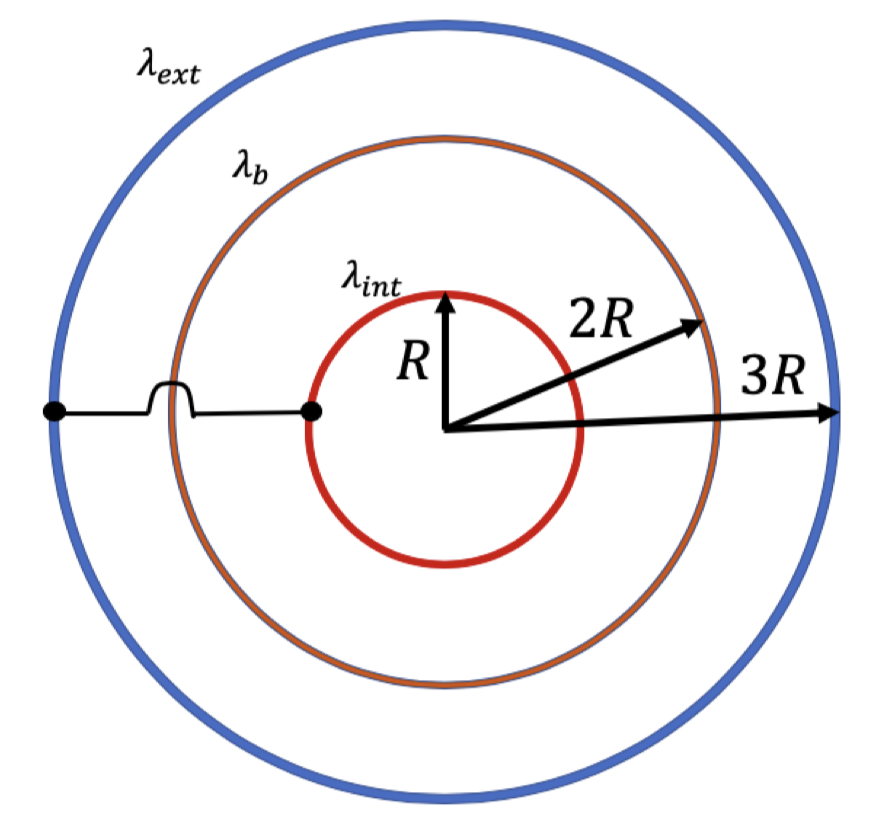
\includegraphics[width=0.47\textwidth]{Electroestática/conductores/P6IB.png}
    \end{figure}
    % Completar respuestas con desarrollo y resultados
    Como se tiene que la capa de radio $R$ y la de radio $3R$ están conectadas entonces sus potenciales son iguales, sabiendo esto y con la Ley de Gauss se puede calcular el campo eléctrico y obtener expresiones para los voltajes. Y usando $V(R) - V(2R) = V(3R) - V(2R)$ se puede despejar $\lambda_{int}$. Luego usando que son conductores y comienzan neutrales se tiene $0 = \lambda_{ext} + \lambda_{int} + \lambda_b$, y se puede obtener el valor de $\lambda_{ext}$
    % Completar respuestas con desarrollo y resultados    
    \item Para despejar la capacitancia se ocupa la relación entre energía potencial eléctrica y capacitancia, y además se despeja usando la definición que la relaciona con el voltaje.
    % (Copiado del aux)
    \item Las cargas ($\lambda_{int}, \lambda_{ext} $ y $ \lambda_b$) permanecen donde se encontraban. Con respecto a $\lambda_{nuevo}$, se distribuirá de manera uniforme en la superficie exterior ($r=3R$).
    
    
\end{enumerate}
\newpage

% Potencial
% Problemas de Guia 3 Daniela Mancilla Primavera 2020

\section{Potencial eléctrico}

Se define el potencial electrostático de un campo eléctrico $\Vec{E}$ en un punto $\Vec{r_1}$ como

%Cambio: dr -> dl
\[V(\Vec{r_1}) = -\int^{\Vec{r_1}}_{\Vec{r_o}}\Vec{E}\cdot d\Vec{l}\]

Donde $\Vec{r_o}$ es un punto de referencia arbitrario tal que $V(\Vec{r_o})=0$, es importante hacer notar que en $\Vec{r_o}$ no puede haber cargas. En general el potencial es 0 en el infinito, esto no se cumple para campos generados por cuerpos infinitos. 
\medbreak
%Agregado lo que está abajo
$V(\Vec{r}) = 0 \text{ en infinito} \iff$ estar conectado a tierra. 
\medbreak
Por definición (teorema fundamental del cálculo) el potencial eléctrico es una función continua, independiente de si el campo eléctrico lo es o no.

\subsection{Potencial de una carga puntual}

El potencial dado por una carga puntual $q$ es

\[V(\Vec{r}) = -\int^{\Vec{r}}_{\infty}\Vec{E}\cdot d\Vec{r} = \frac{q}{4\pi\epsilon_o}\frac{1}{\parallel\Vec{r}-\Vec{r_q}\parallel}\]

Por principio de superposición, el potencial dado por una distribución de cargas continua es

\[V(\Vec{r}) = \frac{1}{4\pi\epsilon_o}\int\frac{1}{\parallel\Vec{r}-\Vec{r_q}\parallel}\,dq(r_q)\]

\subsection{Ecuaciones del Potencial}

\begin{itemize}
    \item $\Vec{E} = -\nabla V$
    \item $\nabla^2V = -\frac{\rho}{\epsilon_o}$ (Ecuación de Poisson)
    %\item $\nabla^2V = 0$ (Ecuación de Laplace)
\end{itemize}


\subsection{Problemas}
--------------------------------------------------------


\np
\begin{enumerate}[label=\alph*)]
    \item El potencial (en relación con un punto en el infinito) a media distancia entre dos cargas de igual magnitud y signo opuesto es igual a cero. ¿Es posible traer una carga de prueba del infinito a ese punto medio en forma tal que no se efectúe trabajo en ninguna parte del desplazamiento? Si es así, describa como se puede lograr. Si no es posible, explique por qué.
    \item Si $\Vec{E}$ es igual a cero en todo lugar a lo largo de cierta trayectoria que vaya del punto \textit{A} al \textit{B}, ¿cuál es la diferencia de potencial entre esos dos puntos? ¿Significa esto que es iguala cero en todos los puntos a lo largo de cualquier trayectoria de \textit{A} a \textit{B}? Explique su respuesta.
    \item Si se conoce el potencial eléctrico en un solo punto, ¿se puede determinar $\Vec{E}$ en ese punto? Si es así, ¿cómo? Si no es posible, ¿por qué?
\end{enumerate}

\np
Un cilindro de radio $a$ y de largo infinito, se carga uniformemente con una densidad de carga volumétrica $\rho_0$. Considere un sistema de coordenadas cilíndricas, donde el eje $\hat{z}$ coincide con el eje del cilindro. 
\begin{enumerate}[label=\alph*)]
    \item Calcule el potencial y el campo electrostáticos en los puntos interiores y exteriores del cilindro resolviendo las ecuaciones de Poisson y Laplace respectivamente. Note que tiene que resolver dos ecuaciones de derivadas parciales de segundo orden, para ello necesita imponer las siguientes cuatro condiciones de borde para resolver el problema de forma completa.
    \begin{enumerate}[label=\arabic*)]
        \item El campo eléctrico en el eje es nulo, $\Vec{E}(r=0)=0$. ¿Por qué?
        \item El campo eléctrico en $r=a$ es continuo,\newline $\Vec{E}_{interior}(r=a)=\Vec{E}_{exterior}(r=a)$. ¿Puede ser el campo eléctrico discontinuo? Si es así, ¿en que situaciones?
        \item El potencial eléctrico en $r=a$ es continuo, $V_{interior}(r=a) = V_{exterior}(r=a)$. ¿Puede ser el potencial eléctrico discontinuo? Fundamente su respuesta.
        \item El potencial de referencia en $r=0$ nulo, es decir, $V(r=0) = 0$. ¿Por qué se puede hacer esta elección?
    \end{enumerate}
    \item Determine el campo eléctrico en todo el espacio utilizando el teorema de Gauss. A partir del resultado obtenido, calcule el potencial en todo el espacio y compruebe que coincide con el obtenido en el apartado anterior.
\end{enumerate}


\np
Se tiene una distribución de carga con simetría esférica, caracterizada por dos radios $a$ y $b$, con $a < b$. Para $r < a$ la densidad de carga es constante e igual a $\rho_0$. Por otra parte, para $a < r < b$ hay una densidad de carga que no se conoce, pero se sabe que el potencial total (con referencia nulo en infinito) en esa zona es: 
\[V(a<r<b)=-\frac{k}{6}r^2\]
Además, se sabe que en la cáscara esférica de radio $r=a$ existe una densidad superficial de carga $\sigma_1$ uniforme, y que en $r=b$ otra de valor $\sigma_2$. Los valores de estas densidades no se conocen. Sabiendo que no hay otras distribuciones de carga, se pide determinar:
\begin{enumerate}[label=\alph*)]
    \item El campo y el potencial eléctrico en todo el espacio.
    \item Las densidades $\sigma_1$ y $\sigma_2$.% y $\rho_0$.
    \item El trabajo necesario para llevar una carga $q$ desde $r=a$ hasta $r=b$. 
\end{enumerate}

\np
Considere la siguiente configuración de cargas, ubicadas en los vértices de un cuadrado de lado $a$.

\begin{figure}[H]
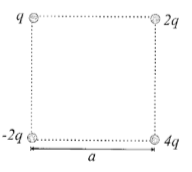
\includegraphics[width=4cm]{Electroestática/Potencial_electrico/p4_potencial.png}
\centering
\end{figure}

\begin{enumerate}[label=\alph*)]
    \item Calcule el trabajo necesario para disponer las cuatro cargas en la configuración mostrada.
    \item ¿Que representa el trabajo?
\end{enumerate}


\newpage
\subsection{Soluciones}


\sol{1}
\begin{enumerate}[label=\alph*)]
    \item \textit{Respuesta:} Si es posible \newline Primero definamos $V(r = \infty)=0$, que es posible al ser una distribución finita de cargas. \\ Ahora notemos que el sistema está compuesto de dos cargas, \textit{q} y \textit{-q} tal que a su distancia media el potencial es cero. Ahora el potencial en un punto cualquiera vendrá dado por \[V(\Vec{r})=\sum_{i=1}^2\frac{q_i}{4\pi\epsilon_o}\frac{1}{\abs{\Vec{r}-\Vec{r_i}}}\] en donde reemplazando los valores de las cargas nos queda (con $r_+$ la distancia a la carga \textit{q} y $r_{-}$ la distancia a la carga \textit{-q}) \[V(\Vec{r})=\frac{q}{4\pi\epsilon_o}\left(\frac{1}{\norma{\Vec{r} - \Vec{r_+}}} - \frac{1}{\norma{\Vec{r} - \Vec{r_{-}}}} \right)\]
    Lo que implica que el trabajo hecho para mover una carga $q_0$ desde un punto a otro será $W_{ext} = q_0 \Delta V = q_0(V(\Vec{r})-V(\infty)) = q_0V(\Vec{r})$, con esto podemos darnos cuenta que si el desplazamiento es a través de la recta perpendicular a la distancia media entre ambas cargas, el trabajo será siempre cero, ya que la distancia en norma hacia ambas cargas será igual, dando cero el potencial en cualquiera de los puntos. 
    
    \item \textit{Respuestas:} Cero y No \newline Sabemos que la diferencia de potencial (\textit{d.d.p}) viene dado por \[V(\Vec{r_b}) - V(\Vec{r_a}) = - \int_{\Vec{r_a}}^{\Vec{r_b}}\Vec{E}\cdot d\Vec{l}\]
    Por lo que si el campo eléctrico es cero en todo el camino, entonces también lo es en $\Vec{r_a}$ y $\Vec{r_b}$ y queda $V(\Vec{r_b}) - V(\Vec{r_a}) = 0$ \newline Tenemos que el potencial en $\Vec{r_a}$ es cero, ya que el campo es cero en ese punto, pero desconocemos si el campo es cero en todo el espacio, por lo que si existe un sector en donde el campo es distinto de cero y se escoge una trayectoria que pase por ese sector se tendrá entonces que la diferencia de potencial \textbf{no} será cero en cualquier punto.
    
    \item \textit{Respuesta:} No \newline Las relaciones entre campo y potencial nos permite despejar uno en función del otro solo si conocemos su expresión general (ya sea global o local), por lo que conociendo un valor específico no se puede obtener el valor del campo. Aunque si se conociera el valor del potencial en un punto, el punto en donde se hace cero y la densidad de carga del espacio, si se podría haciendo uso de la ecuación de Poisson.

\end{enumerate}
\bigbreak
\sol{2}
\begin{enumerate}[label=\alph*)]
    \item \textit{Respuesta:} \newline Para $r < a$, $V(\rho) = -\frac{\rho_0}{4\epsilon_0}\rho^2$ y $\vec{E}(\rho) = \frac{\rho_0}{2\epsilon_0}\rho\hat{\rho}$
    \newline Para $r > a$, $V(\rho) = -\frac{\rho_0a^2}{4\epsilon_0} -\frac{\rho_0a^2}{2\epsilon_0}\ln\left(\frac{\rho}{a}\right)$ y $\vec{E}(\rho) = \frac{\rho_0}{2\epsilon_0}\frac{a^2}{\rho}\hat{\rho}$ 
    
%    \textbf{\textit{Revisar}}
    \begin{enumerate}[label=\arabic*)]
        \item Siguiendo la idea de la Ley de Gauss, tenemos que el flujo corresponde a la cantidad de carga encerrada, pudiéndose despejar el campo en casos de simetría. En este caso notemos que esto es posible, y que en $r=0$ la carga encerrada correspondería a cero, al ser el eje del cilindro. Así tendremos que el campo será cero en ese punto.
        \item Si es posible, si existiera una densidad de carga superficial tal que aumentara bruscamente el campo este sería discontinuo en $r=a$
        \item Como fue explicado al inicio de la sección se tiene que el potencial no puede ser discontinuo. 
        \item Haciendo uso de la lógica en (1), al no haber carga en $r=0$ podemos establecer el punto de referencia ahí. Además es necesario al no poder establecerlo en infinito a causa de la existencia de una distribución infinita de cargas.
    \end{enumerate}
    \bigbreak
    \textit{Solución} \newline
    Tenemos que las ecuaciones de Poisson y Laplace respectivamente son $\nabla^2V = \frac{-\rho}{\epsilon_0}$ y $\nabla^2V = 0$, con $\rho_0$ la densidad de carga del objeto. Además conocemos que $\Vec{\nabla}V = -\Vec{E}$. Donde $\nabla$ representa el gradiente y $\nabla^2$ el laplaciano de $V$.
    
    En este caso, como las coordenadas están en cilíndricas tendremos que usar la divergencia y el gradiente en cilíndricas. Notemos que a causa de que es un cilindro infinito el campo eléctrico solo dependerá de la coordenada $\rho$ por argumentos de simetría, al igual que el potencial, facilitando la aplicación de las ecuaciones para el potencial y el campo eléctrico. 
    
    Analicemos por caso:
    
    I) \boxed{r < a} Utilizamos Poisson
    
    \[\nabla^2V = \frac{-\rho}{\epsilon_0} \implies \frac{1}{\rho}\frac{\partial}{\partial \rho}\left( \rho \frac{\partial V}{\partial \rho}\right) = -\frac{\rho_0}{\epsilon_0}\]
    \[\implies \rho\frac{\partial V}{\partial \rho} = -\frac{\rho_0}{\epsilon_0}\frac{\rho^2}{2} + A \quad (\text{A} \in \mathbb{R} )\]
    \[\implies V(\rho) = -\frac{\rho_0}{4\epsilon_0}\rho^2 + A\ln(\rho) + B \quad (\text{A, B} \in \mathbb{R})\]
    Ocupamos las condiciones de borde entregadas por el problema y despejamos $A$ y $B$,
    \[V(0) = A\ln(0^*) + B = 0 \implies A = B = 0\]
    \[\implies V(\rho) = -\frac{\rho_0}{4\epsilon_0}\rho^2\]
    Ahora haciendo uso del valor de $V(\rho)$ encontrado y de la relación $\vec{E} = -\vec{\nabla}V$, despejamos el campo eléctrico
    \begin{equation}
        \begin{split}
            &\vec{E} = - \vec{\nabla}V \\
            \implies &\vec{E} = - \frac{\partial}{\partial \rho}\left(\frac{-\rho_0 \rho^2}{4\epsilon_0}  \right)\hat{\rho} \\
            \implies &\vec{E} = \frac{\rho_0 \rho^2}{4\epsilon_0}2\rho\hat{\rho}\\
            \implies &\vec{E} = \frac{\rho_0}{2\epsilon_0}\rho\hat{\rho}
        \end{split}
        \nonumber
    \end{equation}
    Obteniéndose $V$ y $\vec{E}$ para $r < a$\\
    
    II) \boxed{r > a} \newline
    Hacemos uso de la ecuación de Maxwell ($\nabla \cdot \vec{E} = \frac{\rho_0}{\epsilon_0}$) donde en nuestro caso $\rho_0 = 0$ al no haber densidad de carga en el espacio fuera del cilindro. Así
    \begin{equation}
        \begin{split}
            &\nabla\cdot\vec{E} = 0\\
            \implies &\frac{1}{\rho}\left( \frac{\partial (E\cdot\rho)}{\partial \rho}\right) = 0\\
            \implies &E\rho = A \quad\quad;A \in \mathbb{R}\\
            \implies &\vec{E} = \frac{A}{\rho}\hat{\rho} \quad\quad;A \in \mathbb{R}
        \end{split}
        \nonumber
    \end{equation}
    Haciendo uso de la continuidad del campo eléctrico en $r = a$ y el valor para $\vec{E}$ encontrado para $r < a$, despejamos el valor de la constante $A$
    \begin{equation}
        \begin{split}
            &\vec{E}_{(r<a)}(a) = \frac{\rho_0}{2\epsilon_0}a\hat{\rho}\\ 
            &\vec{E}_{(r>a)}(a) = \frac{A}{a}\hat{\rho}\\
            \implies &A = \frac{\rho_0a^2}{2\epsilon_0}\\
            \implies &\vec{E}_{(r>a)} = \frac{\rho_0a^2}{2\epsilon_0}\frac{1}{\rho}\hat{\rho}
        \end{split}
        \nonumber
    \end{equation}
    Para encontrar el potencial ahora usamos la relación $\vec{E} = -\vec{\nabla}V$
    \begin{equation}
        \begin{split}
            &\vec{E} = - \vec{\nabla}V\\
            \implies &\frac{\rho_0a^2}{2\epsilon_0}\frac{1}{\rho} = - \frac{\partial (V)}{\partial \rho}\\
            \implies &-\frac{\rho_0a^2}{2\epsilon_0}\ln{\rho} - B = V(\rho) \quad\quad; B \in \mathbb{R}\\
        \end{split}
        \nonumber
    \end{equation}
    Y aplicando la continuidad del potencial en $r =a$, despejamos $B$
    \begin{equation}
        \begin{split}
            &V_{(r<a)}(a) = -\frac{\rho_0}{4\epsilon_0}a^2\\
            &V_{(r>a)}(a) = -\frac{\rho_0a^2}{2\epsilon_0}\ln{a} - B\\
            \implies &B + \frac{\rho_0a^2}{2\epsilon_0}\ln{a} = \frac{\rho_0}{4\epsilon_0}\rho^2\\
            \implies &B = \frac{\rho_0}{4\epsilon_0}a^2 - \frac{\rho_0a^2}{2\epsilon_0}\ln{a}\\
            \implies &V_{(r>a)} = -\frac{\rho_0a^2}{2\epsilon_0}\ln{\rho} -\frac{\rho_0}{4\epsilon_0}a^2 - \frac{\rho_0a^2}{2\epsilon_0}\ln{a}\\
            \implies &V_{(r>a)}(\rho) = -\frac{\rho_0}{4\epsilon_0}a^2 - -\frac{\rho_0a^2}{2\epsilon_0}\ln{\frac{\rho}{a}}
        \end{split}
        \nonumber
    \end{equation}
    
    
    \item A causa de que ya se han hecho ejercicios relacionados con la Ley de Gauss en problemas anteriores solo se dejarán indicaciones de como calcular para este caso. 
    
    Para obtener el valor del campo eléctrico y el potencial haciendo uso del teorema de Gauss ($\int\vec{E}\cdot\vec{dS} = Q_{enc}/\epsilon_0$) hay que sobreponer un cilindro con largo $\gg$ ancho sobre el cilindro ya existente, en el caso $r<a$ existirá una carga encerrada dependiente de $r$ y para $r>a$ existirá una carga constante. 
    
    Luego de haber despejado el campo se utiliza \[V(\vec{r_b}) - V(\vec{r_b}) = -\int_{\vec{r_b}}^{\vec{r_a}}\vec{E}\cdot d\vec{l} \] donde se parte calculando el potencial al interior del cilindro estableciendo $V(r=0) = 0$, y luego ocupando la continuidad en $r=a$ se calcula, de manera similar, el potencial en todo el espacio para $r>a$. Llegando a los resultados puestos en a)
\end{enumerate}
\bigbreak
\bigbreak
\sol{3}\newline % P1 \ Riquelme 2017-1 o P2 | Cordero 2017-2

$a)$ El espacio se divide en 3 subespacios dados por: $r<a$ (1), $a<r<b$ (2) y $b<r$ (3). Usando la ecuación de Poisson (calculada en \textbf{\ref{PoissonEsferas}}) se tiene que el potencial en cada subespacio es

\begin{itemize}
    \item $V_1 = B_1-\frac{A_1}{r}-\frac{\rho_0 r^2}{6\epsilon_o}$
    \item $V_2 = -\frac{k}{6}r^2$
    \item $V_3 = B_3-\frac{A_3}{r}$
\end{itemize}

Donde la densidad de carga en (3) es 0. Sigue encontrar las condiciones de borde para determinar las constantes.
\medbreak
Por ley de Gauss el campo eléctrico en (1) está dado por

\[\Vec{E_1} = \frac{\rho_0}{\epsilon_o}\frac{4\pi r^3}{3}
\frac{1}{4\pi r^2}\hat{r} = \frac{\rho_0r}{3\epsilon_o}\hat{r}\]

luego

\[\frac{\rho_0r}{3\epsilon_o}\hat{r} =
\Vec{E_1} = -\nabla V_1 = \left(
\frac{\rho_0r}{3\epsilon_o}-\frac{A_1}{r^2}
\right)\hat{r}\]
\bigbreak
lo que implica que $A_1 = 0$. Como el potencial es una función continua, se debe cumplir que $V_1(a) = V_2(a)$

\[B_1-\frac{\rho_0 a^2}{6\epsilon_o} = -\frac{k}{6}a^2
\Leftrightarrow
B_1= \frac{\rho_0-k\epsilon_o}{6\epsilon_o}a^2
\]

El campo eléctrico en (2) es

\[\Vec{E_2}=-\nabla V_2=\frac{k}{3}\Vec{r}\]

Para $V_3$, como el potencial en el infinito es nulo, $B_3$ debe ser 0, además, por continuidad se cumple que $V_3(b) = V_2(b)$

\[-\frac{A_3}{b} = -\frac{k}{6}b^2
\Leftrightarrow
A_3 = \frac{k}{6}b^3
\]

El campo eléctrico en (3) es

\[\Vec{E_3}=-\nabla V_3=-\frac{A_3}{r^2}\hat{r}\]

Se tiene así que

\begin{itemize}
    \item $V_1 = \frac{\rho_0-k\epsilon_o}{6\epsilon_o}a^2
    -\frac{\rho_0 r^2}{6\epsilon_o}$
    \item $V_2 = -\frac{k}{6}r^2$
    \item $V_3 = -\frac{kb^3}{6r}$
    \item $\Vec{E_1}=\frac{\rho_0 r}{3\epsilon_o}\hat{r}$
    \item $\Vec{E_2}=\frac{k}{3}\Vec{r}$
    \item $\Vec{E_3}=-\frac{kb^3}{6r^2}\hat{r}$
\end{itemize}
\bigbreak
$b)$ Por ley de Gauss $E_2$ se puede escribir como

\[E_2 = \frac{Q_a+Q_k(r)}{\epsilon_o}\frac{1}{4\pi r^2}\]

Donde $Q_a$ es la carga encerrada por la cáscara de radio $a$ incluyendo la superficie

\[Q_a = \frac{4\pi a^3}{3}\rho_0+4\pi a^2\sigma_1\]
\medbreak
y $Q_k(r)$ es la carga de la segunda capa que hay entre la cáscara de radio $a$ y otra de radio $r$. Como $Q_k(a)=0$, evaluando $E_2$ cuando $r\rightarrow a$ se tiene

\[\frac{k}{3}a = \frac{a}{3\epsilon_o}\rho_0 +
\frac{\sigma_1}{\epsilon_o} \implies \sigma_1 = \epsilon_o\frac{k}{3}a - \frac{a}{3}\rho_0\]

evaluando $E_2$ cuando $r\rightarrow b$ se tiene

\[\frac{k}{3}b = \frac{Q_b}{\epsilon_o}\frac{1}{4\pi b^2}\]

Donde $Q_b$ es la carga encerrada por la cáscara de radio $b$ excluyendo la superficie. Siguiendo la misma lógica, al evaluar $E_3$ cuando $r\rightarrow b$ se obtiene

\[-\frac{k}{6}b = \frac{Q_b}{\epsilon_o}\frac{1}{4\pi b^2}
+ \frac{\sigma_2}{\epsilon_o}\]

De las dos últimas ecuaciones se desprende que

\[\sigma_2 = -\epsilon_o\frac{k}{6}b-\frac{k}{3}b = -\frac{k}{2}b\]

El potencial $V_2$ calculado con la ecuación de Poisson es

\[V_2 = B_2-\frac{A_2}{r}-\frac{\rho_2 r^2}{6\epsilon_o}\]

Con las condiciones de borde $V_1(a) = V_2(a)$ y $V_2(b) = V_3(b)$

\[-\frac{k}{6}a^2 = B_2-\frac{A_2}{a}-\frac{\rho_2 a^2}{6\epsilon_o}\]
\[-\frac{k}{6}b^2 = B_2-\frac{A_2}{b}-\frac{\rho_2 b^2}{6\epsilon_o}\]

Se obtiene que

\[A_2=\frac{ab}{6}(b+a)\left(\frac{\rho_2}{\epsilon_o}-k\right)\]
\[B_2=\frac{b^2+ab+a^2}{6}
\left(\frac{\rho_2}{\epsilon_o}-k\right)\]

Luego

\[\Vec{E_2} = -\nabla V_2 =
-\frac{A_2}{r^2}\hat{r}+\frac{\rho_2 r}{3\epsilon_o}\hat{r}\]

Igualando esto al valor de $\Vec{E_2}$ que ya se tenía se puede obtener el valor de $\rho_2$

\[\frac{kr}{3} =
-\frac{A_2}{r^2}+\frac{\rho_2 r}{3\epsilon_o}
= \frac{ab}{6r^2}(b+a)\left(\frac{\rho_2}{\epsilon_o}-k\right)
+\frac{\rho_2 r}{3\epsilon_o}\]

\[\frac{k}{6r^2}(ab(b+a)-2r^2) = \frac{1}{6r^2}\frac{\rho_2}{\epsilon_o}(ab(b+a)-2r^2)\]

\[k\epsilon_o = \rho_2\]

%Con esto

%\[Q_k(b) = \frac{4\pi(b^3-a^3)}{3}k\epsilon_o\]
%\[Q_b = \frac{4\pi(b^3-a^3)}{3}k\epsilon_o + Q_a\]
%\[\frac{k}{3}b = \frac{(b^3-a^3)k}{b^2}+
%\frac{a^3}{3\epsilon_ob^2}\rho_0+
%\frac{a^2\sigma_1}{\epsilon_0b^2}\]
%\bigbreak

\bigbreak
c) Para encontrar el trabajo necesario para mover una carga $q$ desde $r =a$ hasta $r=b$, se puede usar la identidad $W_{ext} = -q \Delta V$, con $V(r) = -kr^2/6$. Por lo tanto
\[W_{ext} = -q(V(b) - V(a)) = -q\left( -\frac{k}{6}b^2 + \frac{k}{6}a^2 \right) = q\frac{k(a^2 - b^2)}{6}\]

\bigbreak


\sol{4}\newline\newline
\textit{Respuesta:} \newline\newline
a) $W = 0$
\newline
\newline
b) El trabajo representa la energía usada para mover la carga $q_i$ desde infinito hasta su posición final, esta energía es almacenada en el sistema como energía potencial. (más adelante se verá que la energía electrostática está realmente almacenada en los campos eléctricos)

Por lo que este trabajo representa que al mover las cargas a la configuración establecida no se obtiene energía potencial adicional en el sistema.
\newline
\newline
\textit{Solución}
\newline
\newline
Haciendo uso de la ecuación $W = \frac{1}{2}\sum_{i=1}^4q_iV(\Vec{r_i})$ se obtendrá el trabajo total. Notemos que $V(\Vec{r_i})$ corresponde al potencial causado por todas las cargas excepto la $i$, así, para la carga 1 ($q_1 = -2q, \hspace{4px} q_2 = 4q, \hspace{4px} q_3 = 2q \text{  y  } q_4 = q$) se tiene
\[V_{(2,3,4)}(\Vec{r_1}) = \frac{1}{4\pi\epsilon_0}\left[\frac{4q}{a} + \frac{2q}{a\sqrt{2}} + \frac{q}{a} \right] \implies \frac{1}{2}q_1V_{(2,3,4)}(\Vec{r_1})= \frac{-q}{\kte}\left[ \frac{5q}{a} + \frac{2q}{a\sqrt{2}}\right]\]
\newline Para la carga $q_2$ ($q_2 = 4q$) se tiene
\[V_{(1,3,4)}(\Vec{r_2}) = \frac{1}{4\pi\epsilon_0}\left[\frac{-2q}{a} + \frac{2q}{a} + \frac{q}{a\sqrt{2}} \right] \implies \frac{1}{2}q_2V_{(1,3,4)}(\Vec{r_2})= \frac{2q}{\kte} \frac{q}{a\sqrt{2}}\]
\newline Para la carga $q_3$ ($q_3 = 2q$) se tiene
\[V_{(1,2,4)}(\Vec{r_3}) = \frac{1}{4\pi\epsilon_0}\left[\frac{4q}{a} + \frac{-2q}{a\sqrt{2}} + \frac{q}{a} \right] \implies \frac{1}{2}q_3V_{(1,2,4)}(\Vec{r_3})= \frac{q}{\kte}\left[ \frac{5q}{a} - \frac{2q}{a\sqrt{2}}\right]\]
\newline Para la carga $q_4$ ($q_4 = q$) se tiene
\[V_{(1,2,3)}(\Vec{r_4}) = \frac{1}{4\pi\epsilon_0}\left[\frac{-2q}{a} + \frac{2q}{a} + \frac{4q}{a\sqrt{2}} \right] \implies \frac{1}{2}q_4V_{(1,2,3)}(\Vec{r_4})= \frac{1}{2}\frac{q}{\kte} \frac{4q}{a\sqrt{2}}\]

Sumando todos los términos encontrados, nos queda que 
\[W = \frac{4q^2}{\kte a \sqrt{2}} - \frac{4q^2}{\kte a \sqrt{2}} = 0\]


\newpage

% Energía
\section{Energía Potencial Electrostática}

\subsection{Trabajo}

Dadas una carga $Q$ que genera un campo eléctrico $\Vec{E}$ y otra carga $q$ ubicada en la posición $\Vec{r_a}$ respecto a un origen arbitrario, el trabajo que debe realizar una fuerza externa para desplazar $q$ a un punto $\Vec{r_b}$ está dado por

%Cambio: dr -> dl
\[W_{ext} = \int^{\Vec{r_b}}_{\Vec{r_a}}\Vec{F_{ext}}\cdot d\Vec{l}
= -q\int^{\Vec{r_b}}_{\Vec{r_a}}\Vec{E}\cdot d\Vec{l}
= q(V(\Vec{r_b})-V(\Vec{r_a}))
\]

Para un sistema compuesto de $n$ cargas puntuales $q_i$ $(i \in [1,...,n])$, el trabajo necesario para armar está configuración (trayendo cada carga desde el infinito) viene dado por

\[W_{ext} = \sum_{i=1}^n\sum_{j>i}^n\frac{q_jq_i}{4\pi\epsilon_o r_{ij}}
= \frac{1}{2}\sum_{i=1}^n\sum_{j\neq i}^n\frac{q_jq_i}{4\pi\epsilon_o r_{ij}}
= \frac{1}{2}\sum_{i=1}^nq_iV(\Vec{r_i})\]

Donde $r_{ij} = \parallel\Vec{r_i}-\Vec{r_j}\parallel$ y $V(\Vec{r_i})$ es el potencial dado por todas las cargas puntuales existentes en el sistema exceptuando $i$.
\medbreak
Hay que notar que este no es el trabajo que realiza el sistema, sino un trabaja externo que se debe realizar para desplazar las cargas bajo efecto del campo eléctrico.
\medbreak
El trabajo efectuado por el agente externo para armar la configuración de cargas queda almacenado como energía potencial electrostática (almacenada en el sistema en su conjunto, no como una suma de cargas independientes).

\subsection{Energía Potencial}

La energía potencial $U$ asociada a una fuerza conservativa $\Vec{F}$ se define como

%Cambio: dr -> dl
\[U (\Vec{r_1})= -\int^{\Vec{r_1}}_{\Vec{r_o}}\Vec{F}\cdot d\Vec{l}\]

De forma que la energía potencial electrostática de una carga $q$ es

\[U_e = qV \implies \Delta U_e = q \Delta V\]

Para un sistema de $n$ cargas es

\[U_e = \frac{1}{2}\sum_{i=1}^nq_iV(\Vec{r_i})\]

Para una distribución de cargas continuas es

\[U_e = \frac{1}{2}\int V(\Vec{r})\, dq(\Vec{r})\]

El principio de superposición no aplica para $U_e$, esto puede entenderse como que en un sistema no sólo hay energía asociada a las cargas, sino que también a la interacción entre las mismas.

\subsubsection{Energía de un Campo Eléctrico}

La energía potencial electrostática también se puede entender como energía almacenada en un campo eléctrico

\[U_e = \frac{\epsilon_o}{2}\left(
\oint V\Vec{E}\cdot d\Vec{S}
+\int \parallel\Vec{E}\parallel^2\, d\V
\right)\]

Integrando en todo el espacio

\[U_e = \frac{\epsilon_o}{2}\int \parallel\Vec{E}\parallel^2\, d\V\]

$d\V$ es diferencial de volumen.

\subsection{Teorema trabajo-energía cinética y su relación con la energía potencial}

El teorema trabajo-energía cinética nos dice que trabajo realizado por la fuerza neta, aplicada a una partícula de carga $q$, es igual al cambio de energía cinética
\[W = \Delta K\]

Y debido a que la fuerza externa es conservativa, se tiene que $\Delta K = \Delta U_e$, con lo que se puede concluir que
\[W_{ext} = \Delta U_e = q \Delta V\]
En el caso de la fuerza eléctrica, haciendo uso de la relación $\Vec{F}_{ext} = -\Vec{F}_{el\Acute{e}ctrica}$ se puede obtener que $ W_{elec} = -\Delta U_e =-q\Delta V$

\newpage
\subsection{Problemas}
--------------------------------------------------------
\\

\np
Dos varillas de longitud $L$ están a lo largo del eje $x$, una entre $x=a/2$ y $x=a/2+L$ y la otra entre $x=-a/2$ y $x=-a/2-L$. Cada varilla tiene carga positiva Q distribuida uniformemente.

\begin{enumerate}[label=\alph*)]
    \item Calcule el campo eléctrico producido por la segunda varilla en puntos a lo largo del eje $x$ positivo.
    \item Calcule la magnitud de la fuerza que ejerce una varilla sobre la otra.
\end{enumerate}

\np
\begin{enumerate}[label=\alph*)]
    \item Determine el campo eléctrico en todos los puntos del eje de un anillo de radio $R$ sobre el cual hay una densidad de carga uniforme $\lambda$.
    \item A partir de su resultado anterior, calcule el campo eléctrico creado por una corona circular de radios $R_1$ y $R_2$ ($R_1 < R_2$), sobre la cual hay una densidad de carga uniforme $\sigma$, en los puntos de su eje. Encuentre la magnitud y la dirección del campo eléctrico. Considere puntos arriba y abajo de la corona circular.
    \item ¿A qué se reduce su resultado si $R_1 \longrightarrow 0$? ¿Y si $R_2 \longrightarrow \infty$?
    \item Demuestre que en puntos sobre el eje de la corona (eje $z$) que estén suficientemente cerca del origen, la magnitud del campo eléctrico es aproximadamente proporcional a la distancia entre el centro de la corona circular y el punto. ¿Qué tan cerca es ”suficientemente cerca”?
\end{enumerate}

\np
\begin{enumerate}[label=\alph*)]
    \item Encuentre el campo eléctrico creado por un segmento rectilíneo de longitud $L$ dotado de una densidad de carga uniforme $\lambda$.
    \item A partir del resultado anterior, calcule el campo eléctrico en todos los puntos del espacio, producido por una línea infinita con densidad de carga $\lambda$.
    \item Calcule el flujo de campo eléctrico a través de una superficie cilíndrica cerrada, de largo h y radio R, concéntrica con la línea infinita.
    \item  Se tienen dos líneas infinitas con densidad de carga $\lambda$ y $-\lambda$, situadas a una distancia $2a$ una de la otra. Encuentre la fuerza por unidad de longitud que se establece entre los dos hilos. ¿Es atractiva o repulsiva?
\end{enumerate}
\newpage
\np
Considere un plano infinito (en las direcciones $x$ e $y$) de grosor $2R$ (en la dirección $z$), cargado con una densidad de carga volumétrica $\rho$ uniforme. Este plano tiene un agujero cilíndrico (cuyo eje coincide con el eje $y$) de radio $R$ sin cargas.
\begin{enumerate}[label=\alph*)]
    \item Determine el campo eléctrico en todo el espacio. Note que debería dividir el resultado en 3 zonas distintas.
    \item Calcule la fuerza que experimenta un alambre de largo $L$ con densidad de carga lineal uniforme $\lambda$ ubicado a una distancia $d$ del plano y extendido en la dirección $z$.
    \item Calcule la fuerza que experimenta un alambre de largo $L$ con densidad de carga lineal uniforme $\lambda$ ubicado a una distancia $d+L/2$ del plano y extendido en la dirección $y$.
\end{enumerate}

\begin{figure}[h]
    \centering
    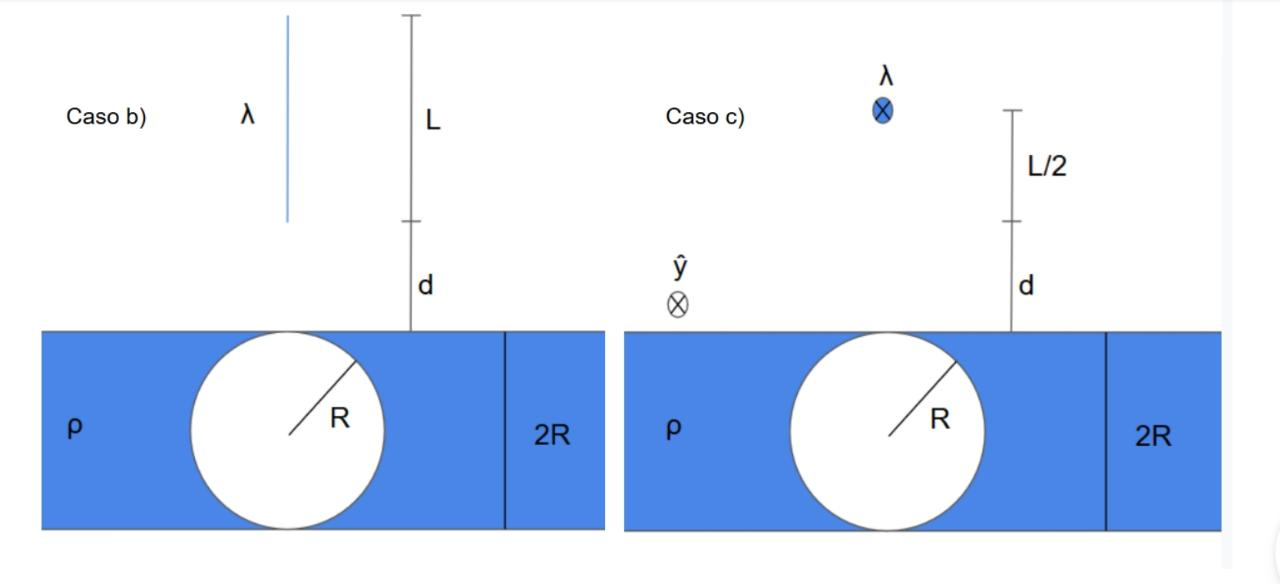
\includegraphics[width=0.9\textwidth]{Electroestática/Campo_electrico/P1 guia2 Mancilla.jpeg}
    \label{fig:P1G2M}
\end{figure}

\np
\begin{enumerate}[label=\alph*)]
    \item Si el campo eléctrico de una carga puntual fuera proporcional a $1/r^3$ en vez de $1/r^2$, ¿seguiría siendo válida la ley de Gauss? Explique su razonamiento. (Sugerencia: considere una superficie esférica centrada en una sola carga puntual).
    \item  Cierta región del espacio limitada por una superficie imaginaria cerrada no contiene carga. ¿El campo eléctrico siempre es igual a cero en todos los puntos de la superficie? Si no es así, ¿en qué circunstancias sería cero en la superficie?
    \item En cierta región del espacio, el campo eléctrico es uniforme. Use la ley de Gauss para demostrar que esa región debe ser eléctricamente neutra; es decir, la densidad volumétrica de carga $\rho$ debe ser igual a cero. Lo contrario, ¿es verdadero? Es decir, en una región del espacio donde no hay carga, ¿debe ser uniforme?
\end{enumerate}

\np
Imagine una esfera de radio R rellena con carga negativa de densidad uniforme y una carga total equivalente a la carga de dos electrones, es decir, $-2e$. En el interior de esta gelatina de carga negativa, se encuentran dos protones, cada uno de ellos de carga $e$. Asuma que, a pesar de la presencia de los protones, la distribución de carga negativa se mantiene uniforme. ¿Dónde deben ubicarse los protones de modo que la fuerza en cada uno de ellos sea nula? Para responder esta pregunta, siga estos pasos:
\begin{enumerate}[label=\alph*)]
    \item Calcule el campo eléctrico producido por los electrones.
    \item Calcule la fuerza de Coulomb neta sobre uno los protones.
    \item Determine la condición de equilibrio y concluya.
\end{enumerate}


\newpage
\subsection{Soluciones}

\sol{1}\newline\newline
$a)$ En un cascarón esférico se tiene simetría $\Vec{E}(\Vec{r}) = E(r)\hat{r}$, por lo tanto, usando ley de Gauss el campo eléctrico del cascarón es 0 si $r<R$, dado que al interior la carga es nula, y para $r>R$ está dada por

\[\Vec{E}(\Vec{r})=\frac{Q}{\epsilon_o}\frac{1}{4\pi r^2}\hat{r}\]

Utilizando la expresión para la energía almacenada en el campo eléctrico se tiene que

\[U_e = \frac{\epsilon_o}{2}\int \parallel\Vec{E}\parallel^2\, dV
= \frac{\epsilon_o}{2}\int \frac{Q^2}{16\epsilon_o^2\pi^2 r^4} \, d\V
\]
\[\,\,\,
= \frac{Q^2}{32\pi^2\epsilon_o}\int^{2\pi}_0\int^{\infty}_R\int^\pi_0 \frac{sin(\theta)}{r^2} \, d\theta drd\phi
\]
\[
= \frac{Q^2}{32\pi^2\epsilon_o}\int^{2\pi}_0\int^{\infty}_R \frac{2}{r^2} \, drd\phi
\,\,\,\,\,\,\,\,\,\,\,\,\,\,\,\,\,\,\,\,\,\,\,\,\]
\[
= \frac{Q^2}{32\pi^2\epsilon_o}\int^{2\pi}_0\frac{2}{R}\, d\phi
\,\,\,\,\,\,\,\,\,\,\,\,\,\,\,\,\,\,\,\,\,\,\,\,\,\,\,\,\,\,\,\,\,\,\,\,\,\,\,\,\,\,\,\]
\[
= \frac{Q^2}{32\pi^2\epsilon_o}\frac{4\pi}{R}
\,\,\,\,\,\,\,\,\,\,\,\,\,\,\,\,\,\,\,\,\,\,\,\,\,\,\,\,\,\,\,\,\,\,\,\,\,\,\,\,\,\,\,\,\,\,\,\,\,\,\,\,\,\,\,\,\,\,\,\,\,\]
\[
= \frac{Q^2}{8\pi\epsilon_oR}\,\,\,
\,\,\,\,\,\,\,\,\,\,\,\,\,\,\,\,\,\,\,\,\,\,\,\,\,\,\,\,\,\,\,\,\,\,\,\,\,\,\,\,\,\,\,\,\,\,\,\,\,\,\,\,\,\,\,\,\,\,\,\,\,\,\,\,\,\,\]
\medbreak
*Para $r<R$ la integral es nula
\bigbreak

$b)$ Se pide encontrar la energía por medio del potencial.
\medbreak
El potencial del cascarón está dado por

\[V(R) = -\int^R_\infty\Vec{E}\cdot d\Vec{r}
= -\int^R_\infty\frac{Q}{4\pi\epsilon_o r^2}\,dr
= \frac{Q}{4\pi\epsilon_o R}\]
\medbreak
Con esto, la energía potencial electrostática es

\[U_e = \frac{1}{2}\int\frac{Q}{4\pi R^2}V(R)\,dS
= \frac{Q^2}{32\pi^2\epsilon_o R}\int^{2\pi}_0\int^\pi_0sin(\theta)\,d\theta d\phi
= \frac{Q^2}{8\pi\epsilon_oR}\]


\newpage

% Conductores
\section{Materiales Conductores}

Se llama conductores a aquellos materiales que poseen cargas libres de moverse en su volumen. Las carga se desplazan al aplicarse un campo eléctrico, las positivas en el sentido del campo y las negativas en sentido opuesto.

Si un conductor siente un campo eléctrico externo $\Vec{E_{ext}}$, sus cargas se desplazarán, formando polos positivos y negativos producto de los cuales se genera un campo eléctrico inducido dentro del material. El campo eléctrico total en el conductor es la suma del campo externo y el inducido.

\[\Vec{E} = \Vec{E}_{ext}+\Vec{E}_{ind}\]

\subsection{Equilibrio Electroestático}

Un conductor está en equilibrio electroestático cuando no presenta movimiento de cargas. En este estado se verifica que:

\begin{itemize}
    %Agregado relación entre E_ind y E_ext
    \item El campo eléctrico al interior del conductor es nulo, $\Vec{E}_{ind} = -\Vec{E}_{ext}$
    \item La carga neta al interior del conductor es nula, $\rho = 0$
    \item Sólo las superficies del conductor pueden poseer carga no nula
    \item El campo eléctrico producto de la carga superficial es normal a la superficie
    \[\Vec{E}=\frac{\sigma}{\epsilon_o}\hat{n}\]
    \item El potencial en el conductor es constante 
\end{itemize}

\subsection{Energía}

Para un sistema formado por $n$ conductores con cargas $\{Q_k\}^n_{k=1}$ y potenciales $\{V_k\}^n_{k=1}$, la energía potencial electrostática es

\[U_e = \frac{1}{2}\sum^n_{k=1}V_kQ_k\]

\subsection{Conductores Huecos}

Para un conductor de carga $Q$ con un agujero en su interior en equilibrio electroestático, se tiene que

\[Q = \int_{S_I}\sigma_I\,dS\,+\int_{S_E}\sigma_E\,dS\]

Donde $S_I$ es la superficie interior y $S_E$ la exterior.

\subsubsection{Carga Interior}

Si en el interior del agujero hay una carga $q$, entonces $\sigma_I$ no es necesariamente uniforme mientras que $\sigma_E$ sí lo es, y se verifica que

\[\int_{S_I}\sigma_I\,dS = -q\]
\[\int_{S_E}\sigma_E\,dS=Q-\int_{S_I}\sigma_I\,dS = Q+q\]

\subsubsection{Carga Exterior}

Si hay una carga al exterior del conductor, $S_E$ apantalla el efecto de $\Vec{E}_{ext}$ sobre $S_I$, de forma de $\sigma_I = 0$. (Funciona como una jaula de Faraday)

\subsection{Condensadores}

Se denomina condensador a sistema compuesto por 2 conductores con carga de igual magnitud y signo opuesto tales que su forma y posición relativa son fijas. En un condensador con cargas $Q_A = Q$ y $Q_B = -Q$ con $Q>0$, dado que la geometría del sistema es fija, se verifica que $\Vec{E}$ es proporcional a $Q$ ($\Vec{E}\propto Q$), en consecuencia la diferencia de potencial, dada por

\[\Delta V = V_A-V_B=\int^A_B \Vec{E} \cdot d\Vec{r}\]

también es proporcional a $Q$. En este caso como $Q_A$ es positivo $V_A > V_B$, puesto que el potencial decrece en el sentido del campo eléctrico (de carga positiva a negativa), en el caso general en que se desconoce cual carga es positiva, se tiene $\Delta V = |V_A + V_B|$.

\subsubsection{Capacitancia}

Se define la capacitancia $C$ de un condensador como la constante de proporcionalidad entre $\Delta V$ y $Q$. Depende únicamente de los parámetros geométricos del problema.

\[C=\frac{Q}{\Delta V}\]

\subsubsection{Energía en un Condensador}

La energía potencial electrostática en un condensador está dada por

\[U_e = \frac{1}{2}Q\Delta V = \frac{1}{2}C(\Delta V)^2=\frac{Q^2}{2C}\]

\subsubsection{Condensadores en paralelo}
Una cantidad $n$ de condensadores se encuentran conectados en paralelo cuando están conectados por sus dos extremos.
\begin{figure}[H]
    \centering
    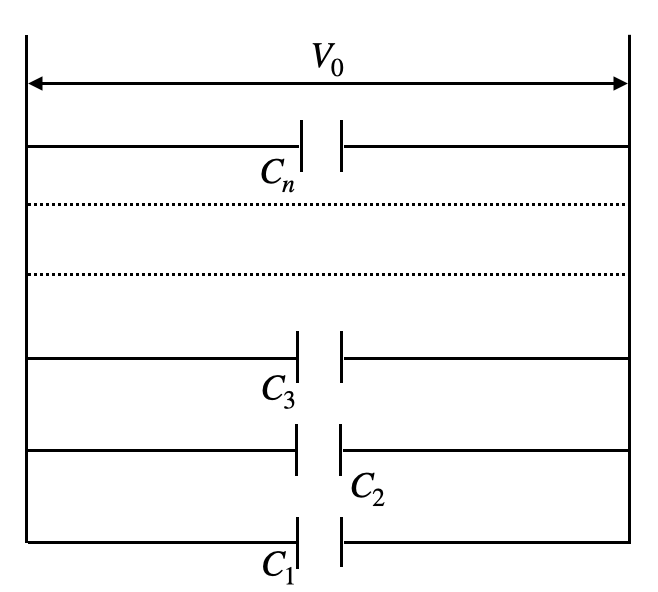
\includegraphics[width=0.42\textwidth]{Electroestática/conductores/condensadores_paralelo.png}
\end{figure}
Los condensadores en paralelo se pueden representar por un condensador equivalente con capacitancia $C_{eq}$, que viene dada por
\[C_{eq} = \sum_{i=1}^nC_i\]
A causa de que todos tienen la misma diferencia de potencial $\Delta V$.

\subsubsection{Condensadores en serie}
Una cantidad $n$ de condensadores se encuentran en serie cuando se conectar por 1 solo extremo entre sí.
\begin{figure}[H]
    \centering
    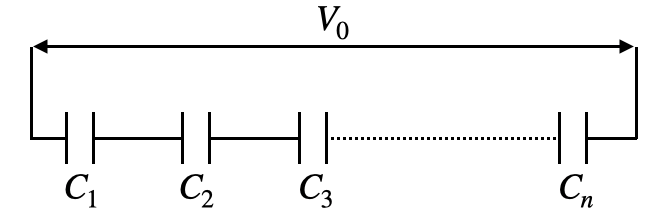
\includegraphics[width=0.55\textwidth]{Electroestática/conductores/condensadores_serie.png}
\end{figure}
Estos se pueden representar por un conductor equivalente con capacitancia $C_{eq}$, que viene dada por
\[C_{eq} = \left( \sum_{i=1}^n\frac{1}{C_i} \right)^{-1} \iff \frac{1}{C_{eq}} =\sum_{i=1}^n\frac{1}{C_i} \]
A causa de que la carga $Q$ es de igual magnitud en todas los conductores.

\newpage


\subsection{Problemas}
--------------------------------------------------------


\np
Una esfera metálica de radio $R$ y carga total $q$ está rodeada por un cascarón esférico metálico de radio interior $a$ y radio exterior $b$. El cascarón tiene carga neta nula. A partir de la configuración expuesta, se le pide:

\begin{figure}[H]
    \centering
    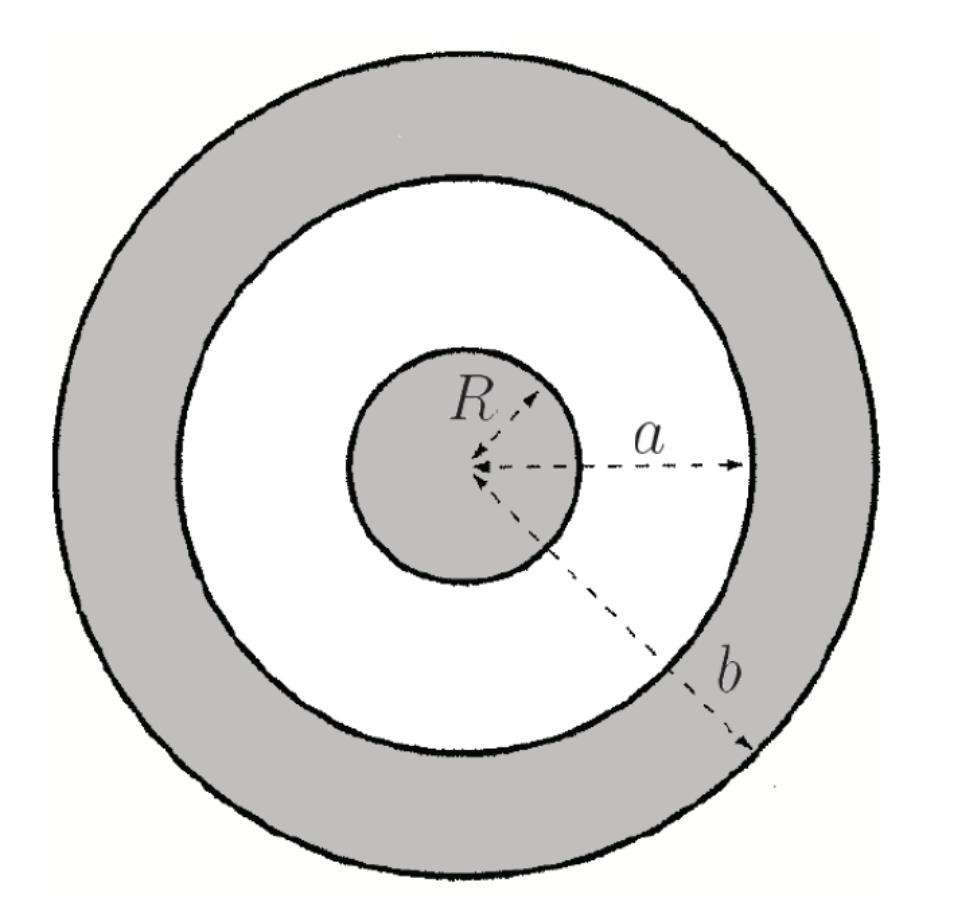
\includegraphics[width=0.6\textwidth]{Electroestática/conductores/P3G4M.jpeg}
\end{figure}

\begin{enumerate}[label=\alph*)]
    \item Encontrar la densidad superficial de carga en cada superficie
    \item Obtener el potencial eléctrico en todo el espacio.
    \item Si el cascarón exterior, se conecta a tierra, bajando su potencial a cero. ¿Cómo cambian sus respuestas anteriores?
    \item Si el cascarón exterior se conecta a un potencial V ¿Cómo cambian sus respuestas anteriores?. En este caso, ¿cuál es la carga neta en el cascarón?
    \item Suponga ahora que se conectan la esfera y el cascarón por un fino hilo conductor. En la nueva situación de equilibrio, ¿cuánto valen el campo eléctrico y el potencial en todo el espacio?
    \item Calcule la variación en la energía electrostática almacenada, como consecuencia de la conexión anterior. ¿Cómo se explica este cambio en la energía?
\end{enumerate}
\bigbreak
\bigbreak

\np
Se tiene un conductor formado por dos esferas de radios $R_1$ y $R_2$ ($R_1 < R_2$), unidas por un cable conductor de largo $L$ ($L \gg R1, R2$). Se distribuye una carga total Q en las esferas.

\begin{enumerate}[label=\alph*)]
    \item ¿Cuánta carga se va a cada esfera? ¿En cuál de las dos es mayor la carga almacenada?
    \item Calcule el potencial del alambre.
    \item ¿En cuál de las dos esferas es mayor la densidad de carga? ¿Y el campo eléctrico en la superficie?
\end{enumerate}

\begin{figure}[H]
    \centering
    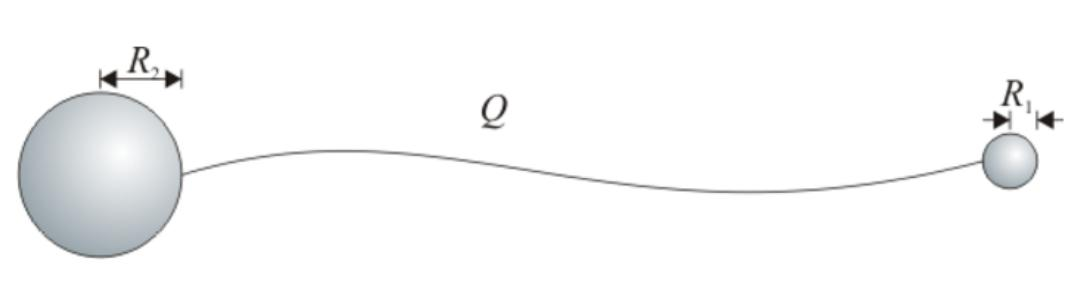
\includegraphics[width=0.7\textwidth]{Electroestática/conductores/P4G4M.jpeg}
\end{figure}
\bigbreak
\bigbreak

\np

Un condensador está hecho de tres capas esféricas concéntricas conductoras de radios $a$, $2a$ y $3a$. En lo que sigue asumiremos que las capas son lo suficientemente gruesas como para distinguir las superficies internas y externas, pero lo suficientemente delgadas como para que no necesitemos saber cuál es su grosor.
\medbreak
Las capas internas y externas están conectadas a tierra: sus potenciales se fijan en cero ($V = 0$). La capa intermedia tiene una carga neta $Q$. Esta carga induce una carga $Q_{in}$ en el borde externo de la capa interna y una carga $Q_{out}$ en el borde interno de la capa externa. Tenga en cuenta que estas cargas se toman de la tierra, por lo que los conductores interno y externo no son eléctricamente neutros.

\begin{figure}[H]
    \centering
    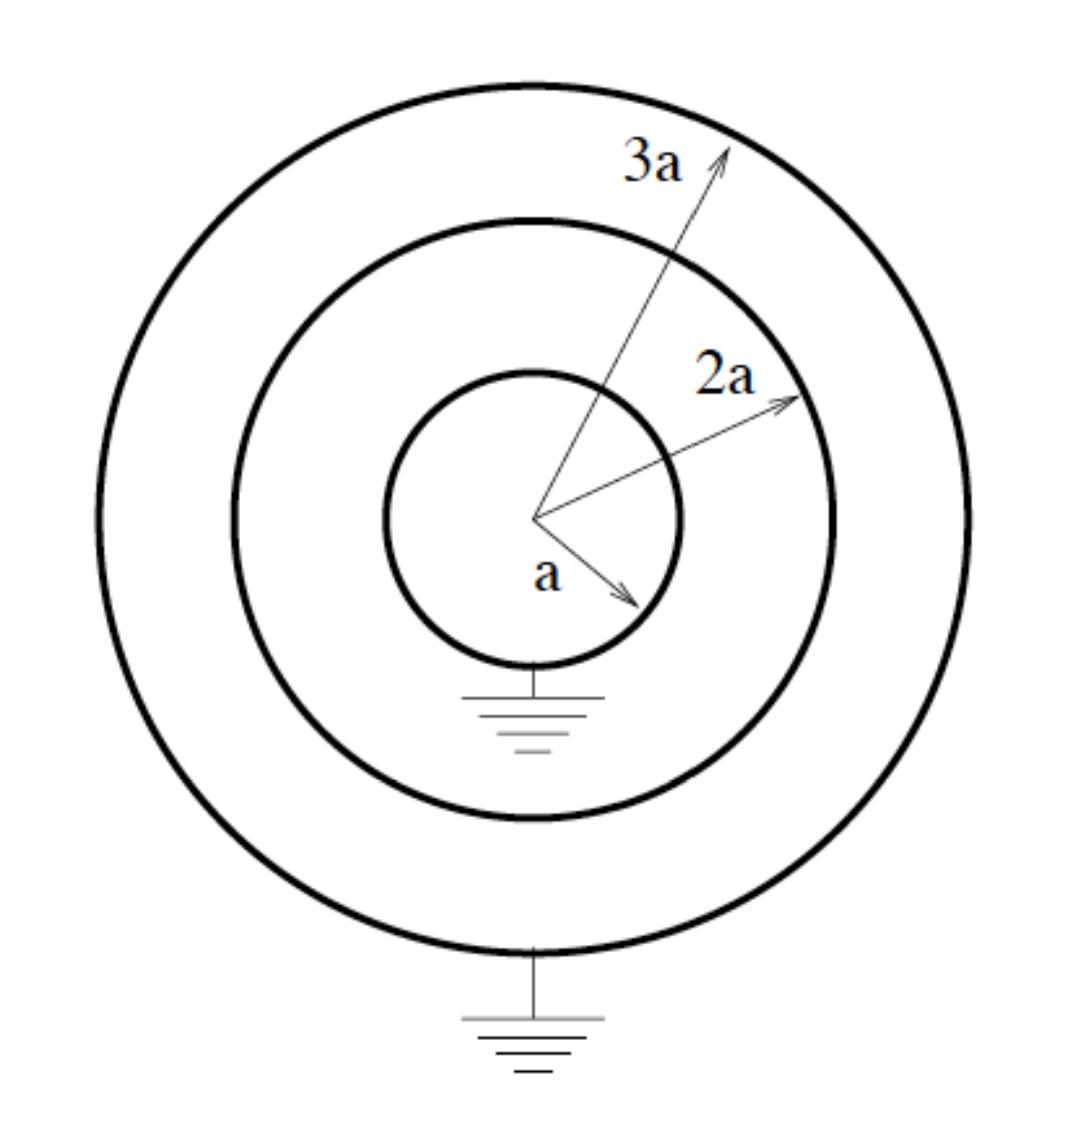
\includegraphics[width=0.6\textwidth]{Electroestática/conductores/P1G5M.jpeg}
\end{figure}

\begin{enumerate}[label=\alph*)]
    \item Calcule el campo eléctrico en todo le espacio en términos de $Q$ y $Q_{in}$.
    \item Encuentre el potencial de la capa intermedia con respecto a la tierra primero yendo de la capa interna a la capa media y luego yendo de la capa externa a la capa media.
    \item encuentre $Q_{in}$ en términos de $Q$.
    \item ¿Cuál es la energía potencial de este sistema?
    \item ¿Cuál es la capacidad de este sistema?
\end{enumerate}

\np

 Un condensador de placas paralelas de área $A$ están a una distancia $x$ entre ellas. Las dimensiones laterales de las placas son mucho más grandes que $x$.

\begin{enumerate}[label=\alph*)]
    \item El condensador se carga a un potencial $V_o$ con una batería tal que las placas se cargan con cargas $+Q$ y $-Q$. Luego, la batería se desconecta. ¿Cuánto trabajo debe realizar una fuerza externa para aumentar la separación una pequeña distancia de $x$ a $x + \Delta x$?
    \item ¿Cuál es el cambio en la energía del condensador desde el estado inicial al final? ¿Se conserva la energía?
    \item Supongamos que la batería hubiera permanecido conectada mientras la fuerza externa aumentaba la separación. ¿Cuánto trabajo realizaría la fuerza externa para aumentar la separación de $x$ a $x + \Delta x$?
    \item ¿Cuál es el cambio en la energía del condensador desde el estado inicial al final en este caso? Muestre que la energía se conserva. 
\end{enumerate}
\bigbreak
\bigbreak
\np

Considere un conductor cilíndrico largo $L$ y de radio $a$, con $L\gg a$. La carga total del cilindro es $Q$ y está distribuida uniformemente en su manto.

\begin{enumerate}[label=\alph*)]
    \item Calcule el campo eléctrico en todo el espacio.
\end{enumerate}

Considere ahora dos conductores cilíndricos de largo $L$, y de radios $a_1$ y $a_2$, separados por una distancia $d$, que es grande comparada con cualquiera de los radios, $d\gg a_1, a_2$. Las cargas totales de los cilindros son $+Q$ y $-Q$.

\begin{figure}[H]
    \centering
    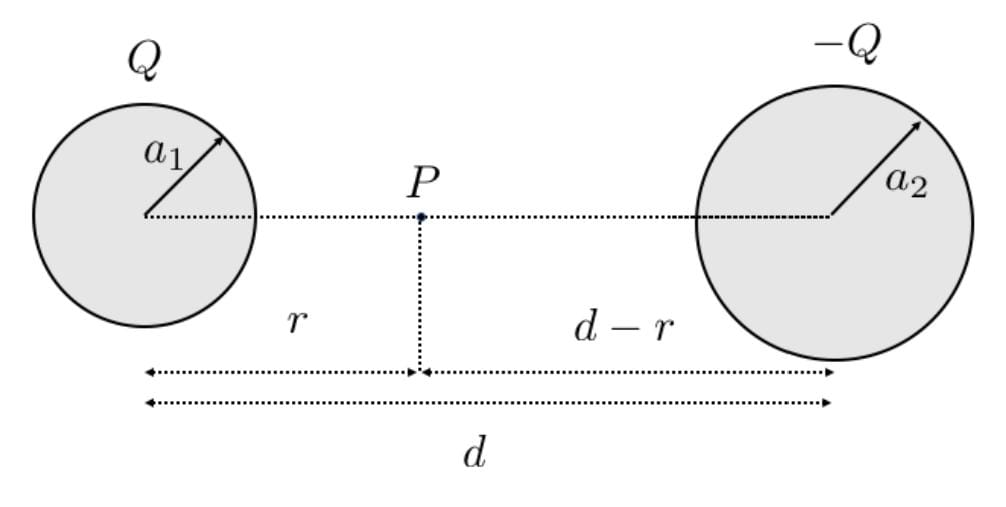
\includegraphics[width=0.6\textwidth]{Electroestática/conductores/P3G5M.jpeg}
\end{figure}

\begin{enumerate}[label=\alph*)]\setcounter{enumi}{1}
    \item Calcule el campo eléctrico en el eje que separa a ambos cilindros, es decir, en el punto $P$ de la figura.
    \item Calcule la diferencia de potencial entre ambos cilindros.
    \item Muestre que la capacitancia por unidad de largo es aproximadamente
    \[C\approx\frac{\pi\epsilon_o}{\ln\left(
    \frac{d}{\sqrt{a_1a_2}}\right)}\]
    \item Suponga que ambos conductores cilíndricos se unen por un cable conductor. Explique qué sucede, y cuál es la situación final del sistema.
\end{enumerate}
\bigbreak
\bigbreak
\np

\begin{enumerate}[label=\alph*)]
    \item Calcule la capacitancia de un condensador cilíndrico de radio interno $R_1$, radio externo $R_2$, y largo $L$.
\end{enumerate}

Ahora considere un condensador consta de tres capas cilíndricas concéntricas con radios $R$, $2R$ y $3R$. Las capas internas y externas están conectadas por un cable conductor, por lo que tienen el mismo potencial. Los conductores comienzan neutros, y luego una batería transfiere carga desde el conductor del medio a los conductores interno/externo.

\begin{enumerate}[label=\alph*)]\setcounter{enumi}{1}
    \item Si la carga final por unidad de longitud en la capa intermedia es $\lambda_b$, ¿Cuáles son las cargas por unidad de longitud en los conductores interior y exterior?
    \item ¿Cuál es la capacitancia por unidad de longitud del sistema?
    \item Si la batería se desconecta, ¿qué pasa con las tres cargas por unidad de longitud en los conductores si se agrega $\lambda_{nuevo}$ al conductor exterior?
\end{enumerate}

\newpage
\subsection{Soluciones}

\sol{1}\newline\newline
$a)$ Al ser metálicas, la esfera y el cascarón son conductores.En equilibrio electrostático, la carga en la superficie interior del cascarón es $-q$ para neutralizar el campo eléctrico de la esfera (que no haya líneas de campo en el conductor) y, dado que su carga total es nula, la carga en la superficie exterior es $q$. Las densidades de carga superficial de la esfera $\sigma_S$, interior del cascarón $\sigma_I$ y exterior del cascarón $\sigma_E$ son uniformes, en el caso de $\sigma_I$ porque la esfera y el cascarón son concéntricos, y están dados por

\[\sigma_S = \frac{q}{4\pi R^2}\]
\[\sigma_I = \frac{-q}{4\pi a^2}\]
\[\sigma_E = \frac{q}{4\pi b^2}\]

$b)$ El espacio está dividido en 4 zonas: al interior de la esfera, $r<R$ (1); entre la esfera y el cascarón, $R<r<a$ (2); interior del cascarón, $a<r<b$ (3); y exterior del cascarón, $b<r$ (4). Como el sistema se compone sólo de conductores y vacío, la densidad volumétrica en todo el espacio es nula. Con esto, utilizando la ecuación de Poisson (calculada en \textbf{\ref{PoissonEsferas}}) el potencial dividido en zonas es

\begin{itemize}
    \item $V_1 = B_1 - \frac{A_1}{r}$
    \item $V_2 = B_2 - \frac{A_2}{r}$
    \item $V_3 = B_3 - \frac{A_3}{r}$
    \item $V_4 = B_4 - \frac{A_4}{r}$
\end{itemize}

Para $r\rightarrow\infty$ el potencial se anula, por lo que $B_4 = 0$, además, dado que en los conductores el potencial es constante, $A_1 = A_3 = 0$.

Los campos eléctricos en (2) y (4) poseen simetría de tipo $\Vec{E}(\Vec{r}) = E(r)\hat{r}$ (demostración en \textbf{\ref{SimetríaEsfera}}), de modo que por ley de Gauss se verifica que

\begin{itemize}
    \item $E_2 = \frac{q}{4\pi\epsilon_o r^2}$
    \item $E_4 = \frac{q}{4\pi\epsilon_o r^2}$
\end{itemize}

Utilizando $\Vec{E} = -\nabla V$ se obtiene

\[\frac{q}{4\pi\epsilon_o r^2} = -\frac{A_2}{r^2} = -\frac{A_4}{r^2}\]

\[A_2 = A_4 = -\frac{q}{4\pi\epsilon_o}\]

Finalmente, por continuidad del potencial

\[V_4(b) = V_3(b) \Rightarrow B_3 = \frac{q}{4\pi\epsilon_o b}\]
\[V_3(a) = V_2(a) \Rightarrow B_2 = \frac{q}{4\pi\epsilon_o}
\left(\frac{1}{b}-\frac{1}{a}\right)\]
\[V_2(R) = V_1(R) \Rightarrow B_1 = \frac{q}{4\pi\epsilon_o}
\left(1+\frac{1}{b}-\frac{1}{a}\right)\]

Se concluye así que

\begin{itemize}
    \item $V_1 = \frac{q}{4\pi\epsilon_o}
\left(1+\frac{1}{b}-\frac{1}{a}\right)$
    \item $V_2 = \frac{q}{4\pi\epsilon_o}\left(
    \frac{1}{r}+\frac{1}{b}-\frac{1}{a}\right)$
    \item $V_3 = \frac{q}{4\pi\epsilon_o b}$
    \item $V_4 = \frac{q}{4\pi\epsilon_o r}$
\end{itemize}
\bigbreak

$c)$ Si se baja el potencial del cascarón a 0, en consecuencia el potencial al exterior de este se anula también

\[V_3 = V_4(b) \Leftrightarrow 0 = -\frac{A_4}{b} \Leftrightarrow A_4 = 0	\Leftrightarrow V_4 = 0\]

Si $V_4 = 0$ entonces $E_4= 0$ y, por ley de Gauss, la carga total encerrada por el cascarón en nula, $\sigma_E = 0$. La carga de la esfera no se ve afectada, de modo que $E_2$ y $A_2$ se mantienen iguales, luego

\[V_2(a) = V_3 \Leftrightarrow B_2 = -\frac{q}{4\pi\epsilon_o a}\]
\[V_2(r) = \frac{q}{4\pi\epsilon_o}\left(\frac{1}{r}
-\frac{1}{a}\right)\]
\[V_1 = V_2(R) = \frac{q}{4\pi\epsilon_o}\left(\frac{1}{R}
-\frac{1}{a}\right)\]

\bigbreak

$d)$ Si $V_3 = V$ entonces

\[V_3 = V_4(b) \Leftrightarrow v = -\frac{A_4}{b} \Leftrightarrow A_4 = -Vb	\Leftrightarrow V_4 = \frac{Vb}{r}\]
\[V_2(a) = V_3 \Leftrightarrow B_2 = V-\frac{q}{4\pi\epsilon_o a}
\Leftrightarrow V_2 = V+\frac{q}{4\pi\epsilon_o}\left(\frac{1}{r}
-\frac{1}{a}\right)\]
\[\Vec{E_4}=-\nabla V_4 = \frac{Vb}{r^2}\hat{r}\]

Para $Q$ la carga total, por ley de Gauss se tiene que

\[E_4= \frac{Q}{4\pi\epsilon_o r^2} = \frac{Vb}{r^2}
\Leftrightarrow Q = 4\pi\epsilon_o Vb\]

Por lo que la carga neta del cascarón es

\[q_c = 4\pi\epsilon_o Vb - q\]

\bigbreak

$e)$ Si se conectan la esfera y el cascarón ambos conformarán un solo conductor y por lo tanto estarán a un mismo potencial. Como la diferencia de potencial es nula, el campo eléctrico en todo el espacio encerrado por el cascarón es 0. Dado que no se produce ningún cambio a la carga total, $E_4$, y por ende $V_4$, son los calculados en $b)$

\[V_1=V_2=V_3=V_4(b)=\frac{q}{4\pi\epsilon_o b}\]
\bigbreak

$f)$ La energía de los conductores desconectados es

\[U_{e1} = \frac{1}{2}(qV_1 + 0\cdot V_3) = \frac{q^2}{8\pi\epsilon_o}
\left(1+\frac{1}{b}-\frac{1}{a}\right)\]

Para los conductores conectados la energía es

\[U_{e2} = \frac{1}{2}qV_3 = \frac{q^2}{8\pi\epsilon_o b}\]

Se tiene $U_{e1} > U_{e2}$ debido a que al conectar los cascarones las cargas se desplazan a causa de un trabajo hecho por el campo, causando que la energía en el sistema disminuya.%para $U_{e1}$ a la energía de los conductores se le agrega la de la interacción entre ambos.

\bigbreak
\bigbreak

\sol{2}\newline\newline
Dado que $L \gg R_1, R_2$ el efecto que tiene cada esfera sobre el potencial de la otra puede ser despreciado. Para $q_1$ y $V_1$ la carga y potencial de la esfera de radio $R_1$, y $q_2$ y $V_2$ la carga y potencial de la esfera de radio $R_2$, se tiene

\[V_1 = \int\frac{\sigma_1}{4\pi\epsilon_o R_1}dS = 
\frac{q_1}{4\pi\epsilon_o R_1}\]

\[V_2 = \frac{q_2}{4\pi\epsilon_o R_2}\]

Como están conectadas, el potencial de las esferas debe ser igual

\[V_1 = V_2 \Leftrightarrow \frac{q_1}{R_1} = \frac{q_2}{R_2}\]

luego

\[Q = q_1 + q_2 = q_1 + \frac{R_2}{R_1}q_1 \Leftrightarrow
q_1 = \frac{R_1 Q}{R_1+R_2}\]

\[q_2 = \frac{R_2 Q}{R_1+R_2}\]

Puesto que $R_1<R_2$, la carga almacenada en la esfera de radio $R_2$ es mayor a la de radio $R_1$

\bigbreak

$b)$ El alambre es parte del conductor por lo que

\[V_{alambre} = V_1 = V_2 = \frac{Q}{4\pi\epsilon_o(R_2+R_1)}\]
\bigbreak

$c)$ La densidad de carga de las esferas es

\[\sigma_1 = \frac{q_1}{4\pi R_1^2} =
\frac{Q}{4\pi R_1(R_1+R_2)}\]
\[\sigma_2 = \frac{q_2}{4\pi R_2^2} =
\frac{Q}{4\pi R_2(R_1+R_2)}\]

Como $R_2 > R_1$, $\sigma_2 < \sigma_1$. El campo eléctrico en las superficies es

\[\Vec{E_1}=\frac{\sigma_1}{\epsilon_o}\hat{r_1}\]
\[\Vec{E_2}=\frac{\sigma_2}{\epsilon_o}\hat{r_2}\]

Donde $\hat{r_i}$ es el vector unitario $\hat{r}$ de las coordenadas esféricas respecto al centro de la esfera de radio $R_i$.
\bigbreak
\bigbreak

\sol{3}\newline\newline
 Usando coordenadas esféricas con origen en el centro de las capas, el espacio se divide en 4 zonas: $r < a$ (1), $a<r<2a$ (2), $2a<r<3a$ (3) y $3a<r$ (4). Las esferas presentan simetría (demostración en \textbf{\ref{SimetríaEsfera}}), por lo que se puede calcular su campo eléctrico con ley de Gauss. Como el sistema comprende sólo conductores y vacío $\rho = 0$ en todo el espacio. De la ecuación de Poisson (resuelta en \ref{PoissonEsferas}) se desprende que en cada zona el potencial es de forma
\[V = B-\frac{A}{r}\]


\begin{enumerate}[label=\alph*)]
    \item Como en (1) no hay carga el campo es nulo
    \[E_1 = 0\]
    \item En (2) la carga encerrada es $Q_{in}$, por lo que el campo eléctrico es
    \[\Vec{E_2} = \frac{Q_{in}}{4\pi\epsilon_o r^2}\hat{r}\]
    \item En (3) la carga encerrada es $Q_{in}+Q$, por lo que el campo eléctrico es
    \[\Vec{E_2} = \frac{Q_{in}+Q}{4\pi\epsilon_o r^2}\hat{r}\]
    \item Para que no haya campo eléctrico al interior del conductor exterior se debe cumplir que $Q_{out} = -(Q+Q_{in})$. Como en el infinito el potencial se anula, en (4) $B=0$ y $V = -\frac{A}{r}$. Igualando $V$ a 0 en $3a$ se obtiene que $A=V=0$ y en concecuencia
    \[E_4 = 0\]


    \item Para $V_2$ el potencial en (2), se verifica que

    \begin{equation}
    \begin{split}
        V_2(r) & = V_2(r) - V_2(a)\\
        & = -\int^r_a\Vec{E_2}\cdot d\Vec{r'}\\
       & = -\int^r_a\frac{Q_{in}}{4\pi\epsilon_o {r'}^2}\,dr'\\
       & = \frac{Q_{in}}{4\pi\epsilon_o r} - \frac{Q_{in}}{4\pi\epsilon_o a}\\
    \end{split}
    \nonumber
    \end{equation}
    Con lo que el potencial en la capa intermedia es

    \[V_2(2a) = -\frac{Q_{in}}{8\pi\epsilon_o a}\]
    \medbreak
    Para $V_3$ el potencial en (3), se verifica que

    \begin{equation}
    \begin{split}
      V_3(r) & = V_3(r) - V_3(3a)\\
      & = -\int^r_{3a}\Vec{E_3}\cdot d\Vec{r'}\\
      & = -\int^r_{3a}\frac{Q_{in}+Q}{4\pi\epsilon_o {r'}^2}\,dr'\\
      & = \frac{Q_{in}+Q}{4\pi\epsilon_o r} - \frac{Q_{in}+Q}{12\pi\epsilon_o a}\\
    \end{split}
    \nonumber
    \end{equation}
    Con lo que el potencial en la capa intermedia es

    \[V_3(2a) = \frac{Q_{in}+Q}{24\pi\epsilon_o a}\]
    \medbreak
    \item Como $V_2(2a)=V_3(2a)$, se tiene que

    \[\frac{Q_{in}+Q}{24\pi\epsilon_o a} = -\frac{Q_{in}}{8\pi\epsilon_o a}\]
    \[\implies Q_{in}=-\frac{1}{4}Q\]
    
    \medbreak
    \item Puesto que las capas exterior e interior están a igual potencial se las puede tomar como un solo conductor de carga $Q_{in} + Q_{out} = -Q$, formando un condensador con la capa intermedia. La capacitancia del sistema está dada por
    
    
    \[C = \frac{Q}{\Delta V} = 32\pi\epsilon_o a\]
    
    Esto también se puede ver como si se tuvieran dos condensadores en paralelo, uno con carga $Q_{in}$ y otro con carga $Q_{out}$ y misma diferencia de potencial $V(2a)$. Al estar en paralelos su capacitancia equivalente sería la suma de las capacitancias individuales, dando el resultado anterior.
    
    La razón de que pueden verse como condensadores en paralelo yace en que poseen el mismo potencial en ambos extremos, en uno están a potencial $V=0$ y en el otro a potencial $V = V(2a)$. En la siguiente imagen se visualiza de manera circuital
    
    \begin{figure}[H]
        \centering
        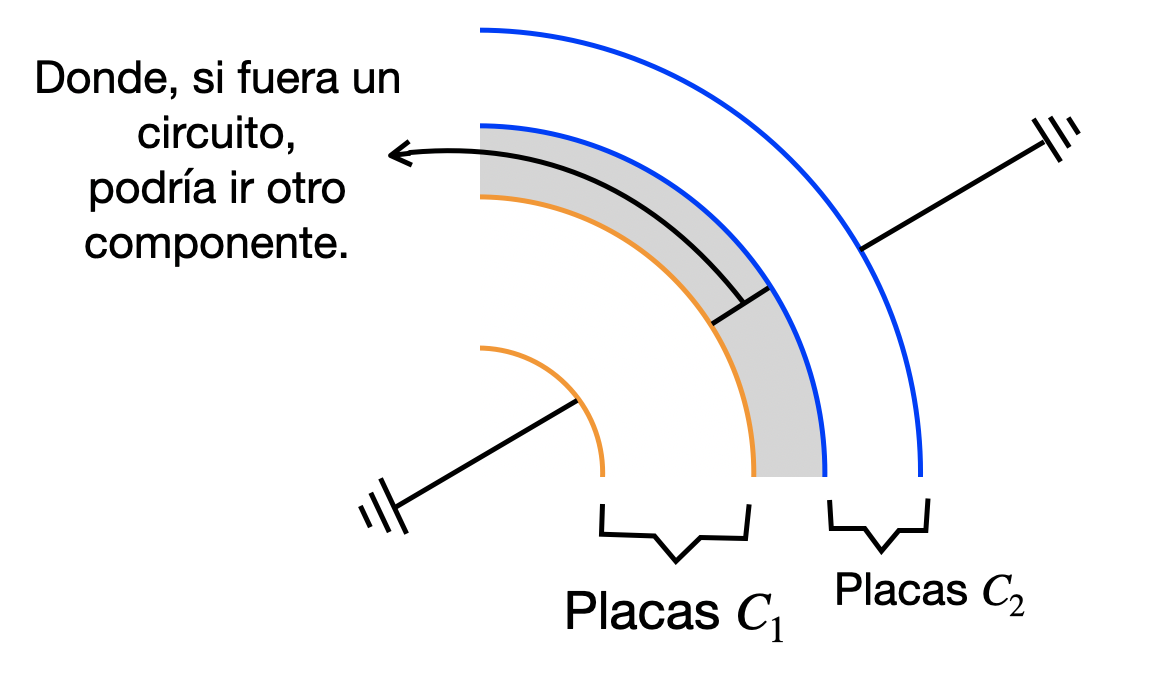
\includegraphics[width=0.5\textwidth]{Electroestática/conductores/P3IG.png}
    \end{figure}
    
    En la figura anterior el conductor de radio $a$ es el inferior izquierdo, el conductor de radio $2a$ está representado por el conductor 'con anchura' de color gris, y el conductor de radio $3a$ es el superior derecho. Las conexiones con 3 líneas representan conexiones a tierra. Y los condensadores son representados el primero con color amarillo-naranjo y el segundo con color azul. 
    
    \medbreak
    \item El sistema está compuesto por 3 conductores y 2 condensadores, como las capas interna y externa tienen potencial nulo, la energía queda dada sólo por la capa intermedia

    \[U_e = \frac{1}{2}V_2(2a) = \frac{1}{8}\frac{Q^2}{8\pi\epsilon_o a}\]
    
    Esto es equivalente a calcular la capacitancia de un condensador equivalente y, haciendo uso de $V(2a)$, obtener la energía potencial con
    $U_e = \frac{1}{2}C\Delta V^2$. 

\end{enumerate}
\bigbreak
\bigbreak
\sol{4}\newline
% Podriamos especificar la alineación de las placas y agregar imagen

\begin{enumerate}[label=\alph*)]
    %a
    \item Como las dimensiones laterales de las placas son mucho más grandes que $x$, se puede aproximar el campo eléctrico de una de las placas al de un plano infinito

    \[\Vec{E} = \frac{Q}{2A\epsilon_o}\hat{x}\]

    ubicando el origen en la placa de carga $Q$, el trabajo par desplazar la placa de carga $-Q$ en $\Delta x$ es

    \begin{equation}
        \begin{split}
            W_{ext} &= Q\int^{x+\Delta x}_x \Vec{E}\cdot d\Vec{r}\\
            & = Q\int^{x+\Delta x}_x\frac{Q}{2A\epsilon_o}\,dr\\
            & = \frac{Q^2}{2A\epsilon_o}\Delta x\\
        \end{split}
        \nonumber
    \end{equation}
    \medbreak
%b
    \item Por teorema de trabajo-energía, se cumple que la diferencia de energía potencial es igual al trabajo hecho por la fuerza externa, por lo que

    \[\Delta U_e = W = \frac{Q^2}{2A\epsilon_o}\Delta x\]
    Notemos que al ser el trabajo positivo, la fuerza externa está inyectando energía al sistema, por lo que se tiene que no se conserva la energía del sistema al aumentar la separación entre las placas por un $\Delta x$
    
    La energía potencial del sistema también se puede calcular haciendo uso del condensador, donde $U_e = \frac{1}{2}Q\Delta V = \frac{Q^2}{2C}$. Como se tiene que la carga de las placas no cambia, entonces se tiene que $C$ y $\Delta V$ han de cambiar. En específico, como se separan las placas $C$ pasa a ser $\frac{\epsilon_o A}{x+\Delta x}$ (calculado en \ref{C:placas}).
%c Aux_5 Daniela Mancilla Otoño 2020
    \item Siguiendo la idea del párrafo anterior, si es que al realizar trabajo cambia la energía del sistema, lo que implica un cambio en el condensador, (carga o diferencia de potencial) entonces al mantener la batería conectada se mantendrá la diferencia de potencial igual. Con esto en mente, entonces será necesario que la carga del condensador cambie.
    
    \begin{equation}
    \begin{split}
        W_{ext} &= \int^{x+\Delta x}_x Q\Vec{E}\cdot d\Vec{r}\\
        & = \int^{x+\Delta x}_x \frac{Q^2}{2A\epsilon_o}\,dr\\
        & = \int^{x+\Delta x}_x
        \frac{(CV_o)^2}{2A\epsilon_o}\,dr\\
        & = \int^{x+\Delta x}_x
        \frac{\epsilon_o AV_o^2}{2r^2}\,dr\\
        &=\frac{\epsilon_o AV_o^2}{2}\left(
        -\frac{1}{x+\Delta x}+\frac{1}{x}\right)\\
        &=\frac{\epsilon_o AV_o^2\Delta x}{2x(x+\Delta x)}
    \end{split}
    \nonumber
    \end{equation} 
    
    \medbreak

%d
    \item La energía potencial eléctrica inicial es
    
    \[U_i = \frac{1}{2}C_iV_o^2 = \frac{\epsilon_o A}{2x}V_o^2\]
    
    la energía potencial final es
    
    \[U_f = \frac{1}{2}C_fV_o^2 = 
    \frac{\epsilon_o A}{2(x+\Delta x)}V_o^2\]
    
    de modo que
    
    \[\Delta U = U_f-U_i = -\frac{\epsilon_o AV_o^2\Delta x}{2x(x+\Delta x)}\]
    
    % Hay que mostrar que la energía que se conserva

\end{enumerate}

\bigbreak
\bigbreak

\sol{5}\newline

\begin{enumerate}[label=\alph*)]
    \item El campo eléctrico en todo el espacio puede ser obtenido haciendo uso de la Ley de Gauss y de la definición de campo eléctrico, debido a lo que será pedido en los siguientes incisos solo será calculado en el caso $\rho > a$ y $\abs{z} < L/2$. Donde se están usando coordenadas cilíndricas y el centro del cilindro como eje.\\
    
    Partamos calculando la densidad superficial de carga, la densidad de carga es superficial a causa de que estamos frente a un conductor que no puede tener campo eléctrico interno, con esto tenemos que 
    \[\sigma = \frac{Q}{2\pi aL}\]
    A causa de que está solo en el manto y el área del manto es $2\pi aL$.\\
    
    Haciendo uso de la Ley de Gauss y sabiendo que por simetría (\ref{SimetríaCilindrosInf}) hay solo campo en la dirección $\hat{\rho}$, establecemos un cilindro más grande superpuesto con el original, de radio $\rho$ y altura $h$, con esto
    %no tiene que ser infinito?, no también el largo(altura) puede ser mucha mayor al radio
    \begin{equation}
        \begin{split}
            &\oint_{Manto} \Vec{E}\cdot d\Vec{S} = \frac{Q_{enc}}{\epsilon_0}\\
            \implies &\int E(\rho)dS = \frac{\sigma 2\pi a h}{\epsilon_0}\\
            \implies &E(\rho) \int dS = \frac{\sigma 2\pi a h}{\epsilon_0}\\
            \implies &E(\rho) 2 \pi \rho h = \frac{\sigma 2\pi a h}{\epsilon_0}\\
            \implies &E(\rho) = \frac{\sigma a}{\epsilon_0 \rho}\\
            \therefore \quad &\Vec{E}(\rho) = \frac{\sigma a}{\epsilon_0 \rho}\hat{\rho}
        \end{split}
        \nonumber 
    \end{equation}
    
    \item Sea $\sigma_+$ la densidad superficial del manto del cilindro de radio $a_1$ y $\sigma_-$ la densidad superficial del manto del cilindro de radio $a_2$, tenemos que el campo eléctrico de cada cilindro será
    
    \[\Vec{E}_{a_1} = \frac{\sigma_+ a_1}{\epsilon_0 \rho}\hat{\rho}\]
    \[\Vec{E}_{a_2} = \frac{\sigma_- a_2}{\epsilon_0 \rho}\hat{\rho'}\]
    
    Si calculamos el campo en $P$ debemos sumar ambos campos, y se tiene que $\hat{\rho'} = - \hat{\rho}$, ya que están centrados en distintos ejes los campos, y en $P$ las direcciones son justo contrarias, así
    
    \[\Vec{E}_{\text{en P}} = \left( \frac{\sigma_+ a_1}{\epsilon_0 r} - \frac{\sigma_- a_2}{\epsilon_0 (d-r)} \right)\hat{\rho}\]
    
    \item Para calcular la diferencia de potencial calculamos $V(a_1) - V(d - a_2)$ por definición,
    
    \begin{equation}
        \begin{split}
            V(a_1) - V(d - a_2) &= -\int_{d-a_2}^{a_1}\left[ \frac{\sigma_+ a_1}{\epsilon_0 r} - \frac{\sigma_- a_2}{\epsilon_0 (d-r)} \right]dr\\
            &= -\left.\left[ \frac{\sigma_+ a_1}{\epsilon_0}\ln{(r)} + \frac{\sigma_- a_2}{\epsilon_0}\ln{(d-r)} \right]\right\rvert_{d-a_2}^{a_1}\\
            &\vdots \quad\\ 
            &\approx -\left[ \frac{\sigma_+}{\epsilon_0}a_1\ln{\left( \frac{a_1}{d} \right)} - \frac{\sigma_-}{\epsilon_0}a_2\ln{\left( \frac{a_2}{d} \right)} \right]\\
            \text{Donde en } \vdots \text{ se usó que } &d-a_1 \approx d\text{ y } d-a_2 \approx d\text{, al ser }d \gg a_1\text{ y } d \gg a_2\\
        \end{split}
        \nonumber
    \end{equation}
    
    Reemplazamos $\sigma_+ = Q/(2\pi La_1)$ y $\sigma_- = -Q/(2\pi La_2)$, y nos queda
    
    \begin{equation}
        \begin{split}
            \Delta V &= -\left[ \frac{Q}{2 \pi L\epsilon_0}\ln{\left( \frac{a_1}{d} \right)} + \frac{Q}{2 \pi L\epsilon_0}\ln{\left( \frac{a_2}{d} \right)} \right]\\
            &=\frac{Q}{2 \pi L \epsilon_0}\ln{\left( \frac{d^2}{a_1a_2} \right)}\\
            &=\frac{Q}{\pi L \epsilon_0}\ln{\left( \frac{d}{\sqrt{a_1a_2}} \right)}
        \end{split}
        \nonumber
    \end{equation}
    
    Lo que nos da que la capacitancia del sistema es
    \[C_{tot} \approx \frac{Q}{\Delta V} = \frac{\pi \epsilon_0 L}{\ln{\left( \frac{d}{\sqrt{a_1a_2}} \right)}}\]
    
    \item Como se tiene que nos piden la capacitancia por unidad de largo debemos dividir la capacitancia encontrada por $L$, así
    \[C \approx \frac{\pi \epsilon_0}{\ln{\left( \frac{d}{\sqrt{a_1a_2}} \right)}}\]
    
    \item Está situación es similar a la presentada en el problema 7.2, por lo que las cargas se distribuirían a través de los cilindros dependiendo de las razones entre sus radios, y el potencial se volvería el mismo para ambos.
    
\end{enumerate}

\sol{6}\newline

\begin{enumerate}[label=\alph*)]
    \item Digamos que la capa del radio interno tiene una carga $-Q$ en su cara exterior, y la capa externa una carga $Q$ en su cara interior. Así queda la configuración como en la siguiente imagen
    \begin{figure}[H]
        \centering
        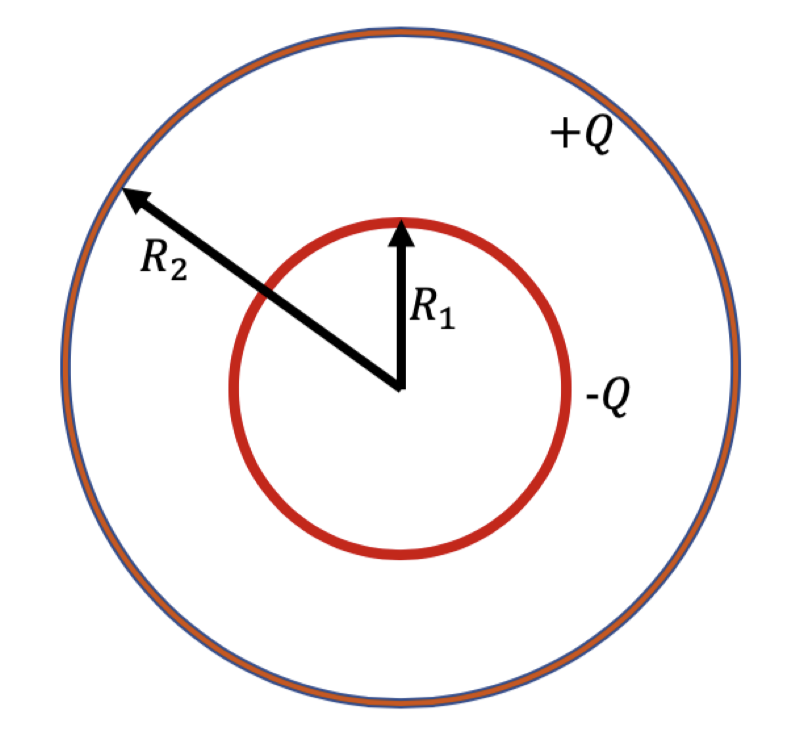
\includegraphics[width=0.47\textwidth]{Electroestática/conductores/P6IA.png}
        \label{fig:sol_6_conduc}
    \end{figure}
    
    Para calcular la capacitancia calculemos la diferencia de potencial entre ambas caras, para esto calculemos el campo eléctrico e integramos de $R_1$ a $R_2$.\\
    
    Usando Ley de Gauss y una superficie Gaussiana de largo $L$ y radio $\rho$, con $R_1 < \rho < R_2$,
    \[\oint_{Manto} \Vec{E}\cdot d\Vec{S} = \frac{Q_{enc}}{\epsilon_0}\]
    \[\implies E(\rho) = \frac{-Q}{2 \pi L \epsilon_0 \rho}\]
    Ahora calculamos la diferencia de potencial,
    \[\Delta V = V(R_2) - V(R_1) =-\int_{R_1}^{R_2}\frac{-Q}{2 \pi L \epsilon_0 \rho}d\rho = \frac{Q}{2\pi L \epsilon_0}\ln{\left( \frac{R_2}{R_1} \right)}\]
    Ahora usando $C = Q/\Delta V$ podemos obtener la capacitancia del sistema
    \[C = \frac{Q}{\Delta V} = \frac{2\pi L \epsilon_0}{\ln{\left( \frac{R_2}{R_1} \right)}}\]
    \text{ }\\     
    % Problema 2 Aux 5 D. Mancilla Otoño2020 (Pauta en Ucursos)
    
    \item \textbf{(Sin valores actualmente)} El nuevo condensador es como el mostrado a continuación
    \begin{figure}[H]
        \centering
        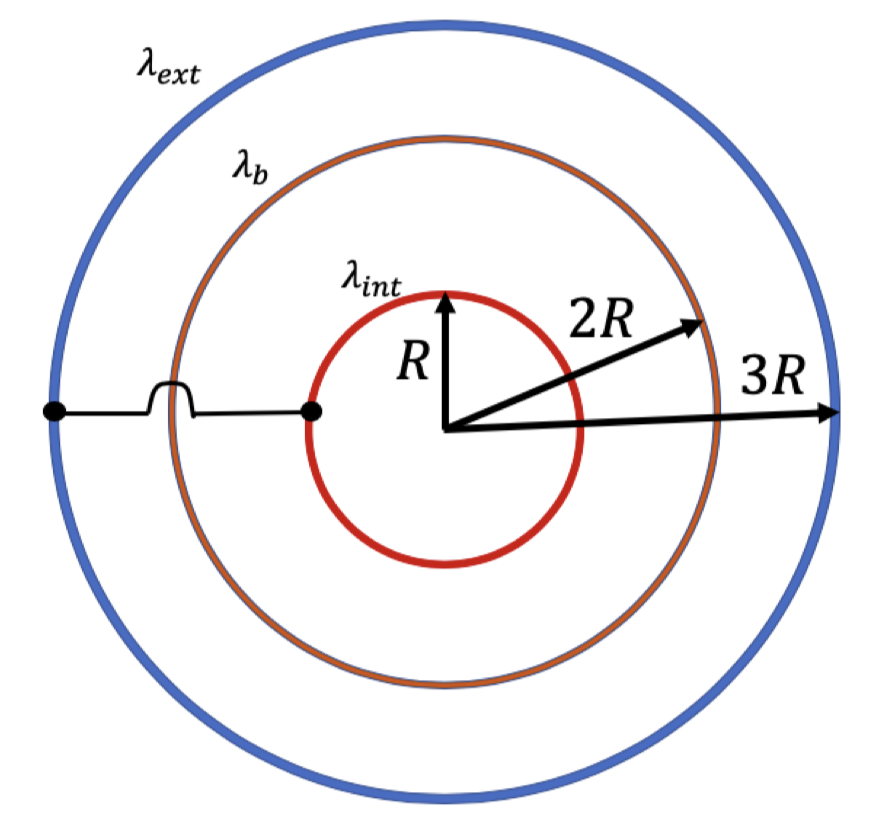
\includegraphics[width=0.47\textwidth]{Electroestática/conductores/P6IB.png}
    \end{figure}
    % Completar respuestas con desarrollo y resultados
    Como se tiene que la capa de radio $R$ y la de radio $3R$ están conectadas entonces sus potenciales son iguales, sabiendo esto y con la Ley de Gauss se puede calcular el campo eléctrico y obtener expresiones para los voltajes. Y usando $V(R) - V(2R) = V(3R) - V(2R)$ se puede despejar $\lambda_{int}$. Luego usando que son conductores y comienzan neutrales se tiene $0 = \lambda_{ext} + \lambda_{int} + \lambda_b$, y se puede obtener el valor de $\lambda_{ext}$
    % Completar respuestas con desarrollo y resultados    
    \item Para despejar la capacitancia se ocupa la relación entre energía potencial eléctrica y capacitancia, y además se despeja usando la definición que la relaciona con el voltaje.
    % (Copiado del aux)
    \item Las cargas ($\lambda_{int}, \lambda_{ext} $ y $ \lambda_b$) permanecen donde se encontraban. Con respecto a $\lambda_{nuevo}$, se distribuirá de manera uniforme en la superficie exterior ($r=3R$).
    
    
\end{enumerate}
\newpage

% Dipolos
\section{Dipolo eléctrico}

Se llama dipolo eléctrico a un sistema compuesto por dos cargas de igual magnitud y signo opuesto.

\begin{figure}[H]
    \centering
    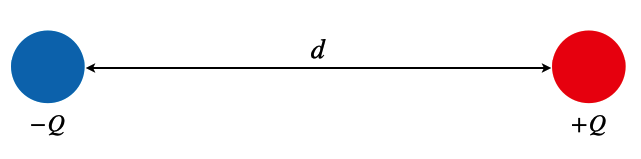
\includegraphics[width=0.59\textwidth]{Electroestática/Dipolos/dipolo.png}
\end{figure}

\subsection{Potencial}

En un sistema de referencia tal que las cargas están en el eje $z$ y el origen se ubica en el punto medio entre ambas el potencial del dipolo es

\begin{equation}
\begin{split}
    V(\Vec{r}) &= \frac{q}{4\pi\epsilon_o}\left(
    \frac{1}{\|\Vec{r}-d/2\hat{z}\|}-
    \frac{1}{\|\Vec{r}+d/2\hat{z}\|}\right)\\
     &= \frac{q}{4\pi\epsilon_o}\left(
    \frac{1}{\sqrt{x^2+y^2+(z-d/2)^2}}-
    \frac{1}{\sqrt{x^2+y^2+(z+d/2)^2}}\right)\\
\end{split}
\nonumber
\end{equation}
\bigbreak
\bigbreak
donde $d$ es la distancia entre las cargas. Si $x,y,z \gg d$ se puede aproximar $V$ por

\begin{equation}
\begin{split}
    V(\Vec{r}) &\approx \frac{q}{4\pi\epsilon_o}\left(
    \frac{1}{\sqrt{x^2+y^2+z^2-zd}}-
    \frac{1}{\sqrt{x^2+y^2+z^2+zd}}\right)\\
    &= \frac{q}{4\pi\epsilon_o}\left(
    \frac{1}{\sqrt{r^2-zd}}-
    \frac{1}{\sqrt{r^2+zd}}\right)\\
    &= \frac{q}{4\pi\epsilon_o r}\left(
    \frac{1}{\sqrt{1-zd/r^2}}-
    \frac{1}{\sqrt{1+zd/r^2}}\right)\\
    &\approx \frac{q}{4\pi\epsilon_o r}\left(
    1+\frac{zd}{2r^2}-\left(1-
    \frac{zd}{2r^2}\right)\right)\\
    &= \frac{qzd}{4\pi\epsilon_o r^3}
\end{split}
\nonumber
\end{equation}
\bigbreak
En coordenadas esféricas, $z=r\cos{\theta}$

\[V(\Vec{r})\approx\frac{qd\cos{\theta}}{4\pi\epsilon_o r^2}\]


\subsection{Momento dipolar}

Para un sistema de $n$ cargas, $\{q_i\}^n_{i=q}$, se define el momento dipolar como

\[\Vec{p}=\sum^n_{i=1}q_i\Vec{r_i}\]

En una distribución de carga continua se tiene

\[\Vec{p}=\int\Vec{r}\,dq(\Vec{r})\]
\bigbreak

El potencial eléctrico generado por un dipolo a \textbf{grandes distancia} es aproximado por

\[V(\Vec{r}) \approx \frac{1}{4\pi\epsilon_o}
\frac{1}{\|\Vec{r}-\Vec{r}'\|^3}\Vec{p}\cdot
(\Vec{r}-\Vec{r}')\]
\bigbreak

donde $\Vec{r}'$ es la posición del punto medio entre las cargas. Lo de grandes distancias es con respecto a $d$ la distancia entre las cargas del dipolo, es por eso que muchas veces se podrá usar esta expresión para puntos no muy alejados del dipolo.\\

El campo eléctrico a partir de este potencial está dado por

\[\Vec{E}= \frac{1}{4\pi\epsilon_o}
\frac{1}{\|\Vec{r}-\Vec{r}'\|^5}\left(3(\Vec{p}\cdot
(\Vec{r}-\Vec{r}'))(\Vec{r}-\Vec{r}')-\|\Vec{r}-\Vec{r}'\|^2\Vec{p}\,\right)\]
\bigbreak
El potencial eléctrico generado por una distribución de cargas arbitraria a grandes distancia se puede aproximar por

\[V(\Vec{r}) \approx V_m + V_d = 
\frac{Q}{4\pi\epsilon_o r}+\frac{\Vec{p}\cdot\Vec{r}}{4\pi\epsilon_o r^3}\]
\bigbreak
donde $V_m$ es la aproximación monopolar y $V_d$ la aproximación dipolar.\\

%Al trabajar con dipolos puede ser útil definir un vector $\Vec{d}$ tal que $\Vec{p}=q\Vec{d}$ y luego hacer tender $\Vec{d}$ a 0

\subsection{Material dieléctrico}

A diferencia de un material conductor donde los electrones están son libres de moverse dentro del material, en un material dieléctrico (o aislante) los electrones están ``atados'' a un átomo o molécula.\\

Cuando un material dieléctrico es puesto en presencia de un campo eléctrico externo, este induce un pequeño momento dipolar en cada átomo o molécula del material, lo que causa que se polarice, dando origen a un campo eléctrico inducido y densidades de carga superficiales. Esto se puede interpretar como que el material está compuesto por dipolos eléctricos.\\

El campo eléctrico neto de un dieléctrico es no nulo.

\[\Vec{E} = \Vec{E}_{ext}+\Vec{E}_{ind} \neq 0\]

\begin{figure}[H]
    \centering
    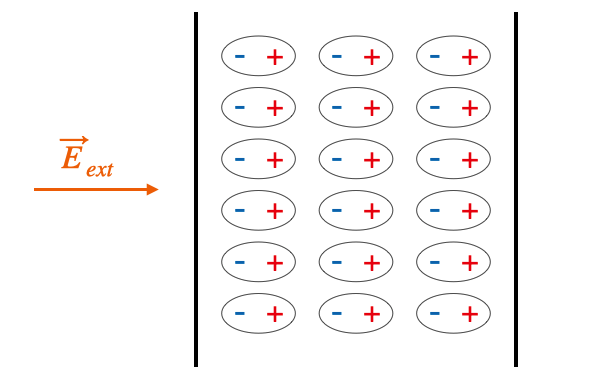
\includegraphics[width=0.6\textwidth]{Electroestática/Dipolos/material_dielectrico.png}
    \caption*{Polarización de los átomos/moléculas del material a causa de un campo $\Vec{E}_{ext}$}
\end{figure}

\subsection{Polarización}

La polarización ($\Vec{P}$) de un material dieléctrico es el momento dipolar por unidad de volumen.

\[d\Vec{p}=\Vec{P}(\Vec{r})d\V\]

Con esto, se puede obtener el potencial de un material polarizado como

\begin{equation}
\begin{split}
    V(\Vec{r}) &= \frac{1}{4\pi\epsilon_o}\int
    \frac{1}{\|\Vec{r}-\Vec{r}'\|^3}(\Vec{r}-\Vec{r}')
    \cdot d\Vec{p}\\
    &= \frac{1}{4\pi\epsilon_o}\int
    \frac{\Vec{P}(\Vec{r}')\cdot(\Vec{r}-\Vec{r}')}{\|\Vec{r}-\Vec{r}'\|^3}\,d\V'\\
    &= \frac{1}{4\pi\epsilon_o}\int\Vec{P}(\Vec{r}')\cdot
    \nabla\left(\frac{1}{\|\Vec{r}-\Vec{r}'\|}\right)\,d\V'\\
    &= \frac{1}{4\pi\epsilon_o}\int\nabla\cdot\left(
    \frac{\Vec{P}(\Vec{r}')}{\|\Vec{r}-\Vec{r}'\|}\right)\,d\V'-\frac{1}{4\pi\epsilon_o}\int
    \frac{\nabla\cdot\Vec{P}(\Vec{r}')}{\|\Vec{r}-\Vec{r}'\|}
    \,d\V'\\
    &= \frac{1}{4\pi\epsilon_o}\oint
    \frac{1}{\|\Vec{r}-\Vec{r}'\|}
    \Vec{P}(\Vec{r}')\cdot d\Vec{S'}-\frac{1}{4\pi\epsilon_o}\int
    \frac{\nabla\cdot\Vec{P}(\Vec{r}')}{\|\Vec{r}-\Vec{r}'\|}
    \,d\V'\\
\end{split}
\nonumber
\end{equation}
\bigbreak
Las últimas integrales se pueden interpretar como potenciales por una carga superficial y una volumétrica. En base a esto, se definen las densidades de carga de polarización:

\begin{equation}
\begin{split}
    &\sigma_p \equiv \Vec{P}(\Vec{r})\cdot\hat{n}\\
    &\rho_p \equiv -\nabla\cdot\Vec{P}(\Vec{r})
\end{split}
\nonumber
\end{equation}
\bigbreak
Con esto, un medio polarizado posee una carga dada por $\sigma_p$ y $\rho_p$. La densidad de carga total al interior del material es

\[\rho_t = \rho_l+\rho_p\]
\bigbreak
donde $\rho_l$ es la densidad de cara libre, la carga ``natural'' del material. La carga total de polarización

\[Q_p=\oint \Vec{P}\cdot d\Vec{S}-\int\nabla\cdot\Vec{P}\,d\V\]
\bigbreak
por teorema de la divergencia es siempre nula.\\

Si $\Vec{P}$ es constante, el potencial se puede calcular como

\[V(\Vec{r})=\frac{1}{\rho_v}\Vec{P}\cdot\Vec{E}_v\]
\bigbreak
donde $\Vec{E}_v$ es un campo eléctrico virtual para una densidad de carga $\rho_v$ uniforme. El vector $\Vec{P}$ se manifiesta sólo dentro del material.

\subsection{Desplazamiento Eléctrico}

Por la primera ecuación de Maxwell se tiene que

\begin{equation}
\begin{split}
    \nabla\cdot\Vec{E} = \frac{\rho_t}{\epsilon_o}
    & \Leftrightarrow \nabla\cdot\Vec{E} = \frac{\rho_l+\rho_p}{\epsilon_o}\\
    &\Leftrightarrow \epsilon\nabla\cdot\Vec{E}=\rho_l -
    \nabla\cdot\Vec{P}\\
    &\Leftrightarrow \epsilon\nabla\cdot\Vec{E}
    +\nabla\cdot\Vec{P}=\rho_l\\
    &\Leftrightarrow\nabla\cdot\left(\epsilon_o
    \Vec{E}+\Vec{P}\right) = \rho_l\\
\end{split}
\nonumber
\end{equation}
\bigbreak
Se define el desplazamiento eléctrico como

\[\Vec{D}=\epsilon_o\Vec{E}+\Vec{P}\]
\bigbreak
Con $\Vec{D}$ se puede definir la primera ecuación de Maxwell en electrostática en medios materiales por

\begin{itemize}
    \item \textbf{Forma diferencial:}
    \[\nabla\cdot\Vec{D}=\rho_l\]
    \item \textbf{Forma integral:}
    \[\oint\Vec{D}\cdot d\Vec{S}=Q_{libre\,encerrada}\]
\end{itemize}

\subsection{Dieléctricos Lineales}

Se llama lineal a un material dieléctrico cuya polarización es proporcional al campo eléctrico, esto es

\[\Vec{P}=\epsilon_o\mathcal{X}_e\Vec{E}\]

A la constante $\mathcal{X}_e$ se le denomina susceptibilidad eléctrica y es característica de cada material.\\

Por la definición de desplazamiento eléctrico se tiene

\begin{equation}
\begin{split}
    \Vec{D} &= \epsilon_o\Vec{E}+\Vec{P}\\
    &= \epsilon_o\Vec{E}+\epsilon_o\mathcal{X}_e\Vec{E}\\
    &= \epsilon_o(1+\mathcal{X}_e)\Vec{E}\\
\end{split}
\nonumber
\end{equation}
\bigbreak
A partir de esto se definen:

\begin{itemize}
    \item \textbf{Permitividad Relativa:}
    \[\epsilon_r=1+\mathcal{X}_e\]
    \item \textbf{Permitividad  Absoluta:}
    \[\epsilon = \epsilon_o\epsilon_r\]
\end{itemize}

Al reemplazar $\Vec{D}=\epsilon\Vec{E}$ en la primera ecuación de Maxwell para materiales se obtiene que

\[\nabla\cdot\Vec{E}=\frac{\rho_l}{\epsilon}\]

\subsubsection{Energía}

La energía de un material dieléctrico lineal se puede calcular como

\[U_e=\frac{1}{2}\int\Vec{E}\cdot\Vec{D}\,d\V\]

integrando sobre todo el espacio.
% Esto tiene sentido y es indicación de una pregunta, pero igual no estoy seguro de si es algo que siempre se cumple. 

% Según yo si, porque si tomas un sistema donde no hay dieléctrico, entonces la permitividad es la del vació y con D=eE, se recupera la ecuación que está en energía potencial electroestática

\subsection{Condiciones de Borde}

Dados dos medios dieléctricos lineales, se llama interfaz a la superficie de contacto entre ambos. El campo eléctrico el materiales se puede descomponer en una parten normal (perpendicular) y otro tangencial (paralela) a la interfaz, estas permiten encontrar las condiciones de borde.

\[\Vec{E}_1 = E_{1n}\hat{n}+E_{1t}\hat{t}\]
\[\Vec{E}_2 = E_{2n}\hat{n}+E_{2t}\hat{t}\]

\subsubsection{Componentes Tangenciales}

Se considera $R$ un camino rectangular infinitesimal (permite ver la interfaz como un plano) cerrado y rectangular, con lados paralelos y perpendiculares a la interfaz que pasa por los dos materiales. La segunda ecuación de Maxwell en electrostática indica que la integral del campo eléctrico en $R$ es nula. Si se hace tender el lado que atraviesa la interfaz a 0, se puede despreciar su contribución a la integral, de modo que


\begin{equation}
\begin{split}
    \oint_R\Vec{E}\cdot d\Vec{l} &= 
    \int_\rightarrow\Vec{E}\cdot d\Vec{l}+
    \int_\uparrow \Vec{E}\cdot d\Vec{l}+
    \int_\leftarrow \Vec{E}\cdot d\Vec{l}+
    \int_\downarrow \Vec{E}\cdot d\Vec{l}\\
    &= \int_\rightarrow\Vec{E}\cdot d\Vec{l}+
    \int_\leftarrow\Vec{E}\cdot d\Vec{l}\\
    &= \int_\rightarrow E_{1t}\,dl+
    \int_\leftarrow E_{2t}\, dl\\
    &= \int_\rightarrow E_{1t}-E_{2t}\, dl\\
    &= 0\\
    &\Rightarrow E_{1t}=E_{2t}\\
\end{split}
\nonumber
\end{equation}
\bigbreak
la componente tangencial del $\Vec{E}$ es continua en la interfaz.

% Puse la imágen para complementar, pero no se si dejarla o no, que opinas? (también creé del desplazamiento)
\begin{figure}[H]
    \centering
    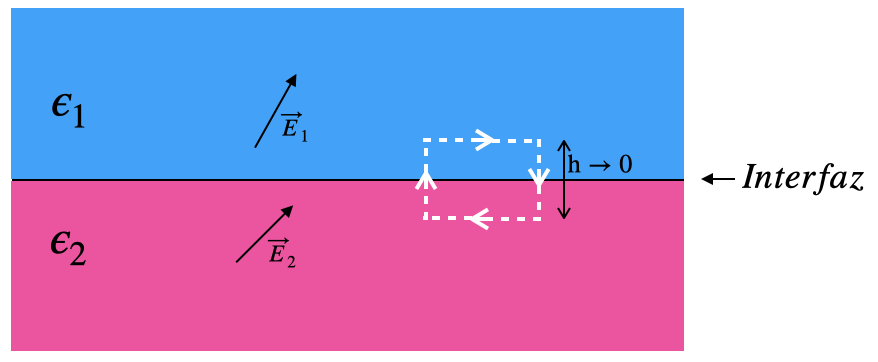
\includegraphics[width=0.5\textwidth]{Electroestática/Dipolos/c_borde_campoe.png}
\end{figure}

\subsubsection{Componentes Normales}

Se considera un cilindro infinitesimal con eje perpendicular a la interfaz y centrado en la misma. Si se hace tender su altura 0, se puede despreciar la superficie del manto y tomar la carga de la interfaz como la única encerrada, de modo que, para $S_1$ la tapa inferior y $S_2$ la tapa superior, por ley de Gauss se tiene que

\begin{equation}
\begin{split}
    \oint\Vec{D}\cdot d\Vec{S}&=\int_{S_1}\Vec{D}\cdot d\Vec{S}+\int_{S_2}\Vec{D}\cdot d\Vec{S}\\
    &=\int_{S_1}D_{1n}\,dS+\int_{S_2}D_{2n}\,dS\\
    &=\int_{S_2}(D_{2n}-D_{1n})\,dS\\
    &=A(D_{2n}-D_{1n})\\
    &=A\sigma_l\\
    &\Rightarrow D_{2n}-D_{1n} = \sigma_l\\
\end{split}
\nonumber
\end{equation}
\bigbreak

donde $A$ es el área de las tapas del cilindro y $\sigma_l$ la densidad de carga de la interfaz.

\begin{figure}[H]
    \centering
    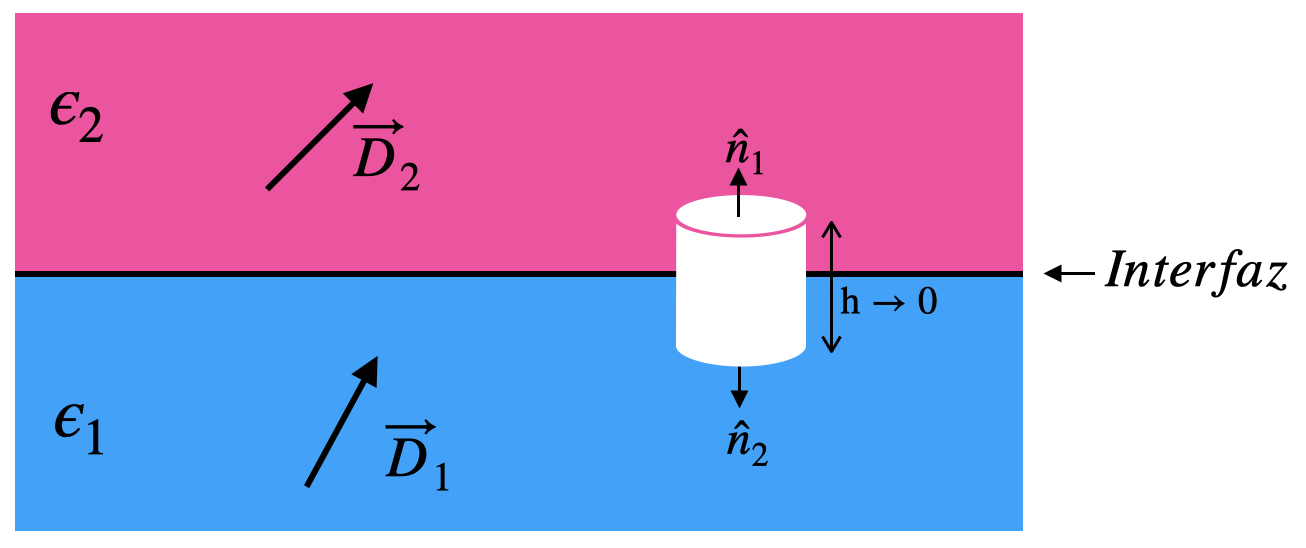
\includegraphics[width=0.5\textwidth]{Electroestática/Dipolos/c_borde_desplaz.png}
\end{figure}

\newpage
\subsection{Problemas}
--------------------------------------------------------
\\

\np
Dos varillas de longitud $L$ están a lo largo del eje $x$, una entre $x=a/2$ y $x=a/2+L$ y la otra entre $x=-a/2$ y $x=-a/2-L$. Cada varilla tiene carga positiva Q distribuida uniformemente.

\begin{enumerate}[label=\alph*)]
    \item Calcule el campo eléctrico producido por la segunda varilla en puntos a lo largo del eje $x$ positivo.
    \item Calcule la magnitud de la fuerza que ejerce una varilla sobre la otra.
\end{enumerate}

\np
\begin{enumerate}[label=\alph*)]
    \item Determine el campo eléctrico en todos los puntos del eje de un anillo de radio $R$ sobre el cual hay una densidad de carga uniforme $\lambda$.
    \item A partir de su resultado anterior, calcule el campo eléctrico creado por una corona circular de radios $R_1$ y $R_2$ ($R_1 < R_2$), sobre la cual hay una densidad de carga uniforme $\sigma$, en los puntos de su eje. Encuentre la magnitud y la dirección del campo eléctrico. Considere puntos arriba y abajo de la corona circular.
    \item ¿A qué se reduce su resultado si $R_1 \longrightarrow 0$? ¿Y si $R_2 \longrightarrow \infty$?
    \item Demuestre que en puntos sobre el eje de la corona (eje $z$) que estén suficientemente cerca del origen, la magnitud del campo eléctrico es aproximadamente proporcional a la distancia entre el centro de la corona circular y el punto. ¿Qué tan cerca es ”suficientemente cerca”?
\end{enumerate}

\np
\begin{enumerate}[label=\alph*)]
    \item Encuentre el campo eléctrico creado por un segmento rectilíneo de longitud $L$ dotado de una densidad de carga uniforme $\lambda$.
    \item A partir del resultado anterior, calcule el campo eléctrico en todos los puntos del espacio, producido por una línea infinita con densidad de carga $\lambda$.
    \item Calcule el flujo de campo eléctrico a través de una superficie cilíndrica cerrada, de largo h y radio R, concéntrica con la línea infinita.
    \item  Se tienen dos líneas infinitas con densidad de carga $\lambda$ y $-\lambda$, situadas a una distancia $2a$ una de la otra. Encuentre la fuerza por unidad de longitud que se establece entre los dos hilos. ¿Es atractiva o repulsiva?
\end{enumerate}
\newpage
\np
Considere un plano infinito (en las direcciones $x$ e $y$) de grosor $2R$ (en la dirección $z$), cargado con una densidad de carga volumétrica $\rho$ uniforme. Este plano tiene un agujero cilíndrico (cuyo eje coincide con el eje $y$) de radio $R$ sin cargas.
\begin{enumerate}[label=\alph*)]
    \item Determine el campo eléctrico en todo el espacio. Note que debería dividir el resultado en 3 zonas distintas.
    \item Calcule la fuerza que experimenta un alambre de largo $L$ con densidad de carga lineal uniforme $\lambda$ ubicado a una distancia $d$ del plano y extendido en la dirección $z$.
    \item Calcule la fuerza que experimenta un alambre de largo $L$ con densidad de carga lineal uniforme $\lambda$ ubicado a una distancia $d+L/2$ del plano y extendido en la dirección $y$.
\end{enumerate}

\begin{figure}[h]
    \centering
    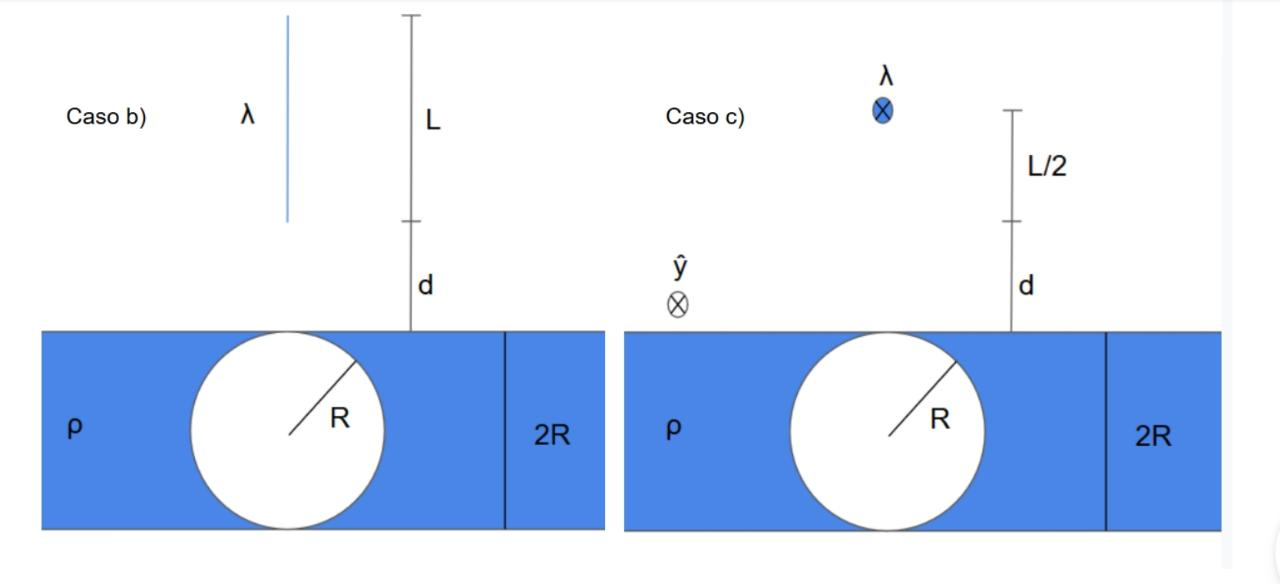
\includegraphics[width=0.9\textwidth]{Electroestática/Campo_electrico/P1 guia2 Mancilla.jpeg}
    \label{fig:P1G2M}
\end{figure}

\np
\begin{enumerate}[label=\alph*)]
    \item Si el campo eléctrico de una carga puntual fuera proporcional a $1/r^3$ en vez de $1/r^2$, ¿seguiría siendo válida la ley de Gauss? Explique su razonamiento. (Sugerencia: considere una superficie esférica centrada en una sola carga puntual).
    \item  Cierta región del espacio limitada por una superficie imaginaria cerrada no contiene carga. ¿El campo eléctrico siempre es igual a cero en todos los puntos de la superficie? Si no es así, ¿en qué circunstancias sería cero en la superficie?
    \item En cierta región del espacio, el campo eléctrico es uniforme. Use la ley de Gauss para demostrar que esa región debe ser eléctricamente neutra; es decir, la densidad volumétrica de carga $\rho$ debe ser igual a cero. Lo contrario, ¿es verdadero? Es decir, en una región del espacio donde no hay carga, ¿debe ser uniforme?
\end{enumerate}

\np
Imagine una esfera de radio R rellena con carga negativa de densidad uniforme y una carga total equivalente a la carga de dos electrones, es decir, $-2e$. En el interior de esta gelatina de carga negativa, se encuentran dos protones, cada uno de ellos de carga $e$. Asuma que, a pesar de la presencia de los protones, la distribución de carga negativa se mantiene uniforme. ¿Dónde deben ubicarse los protones de modo que la fuerza en cada uno de ellos sea nula? Para responder esta pregunta, siga estos pasos:
\begin{enumerate}[label=\alph*)]
    \item Calcule el campo eléctrico producido por los electrones.
    \item Calcule la fuerza de Coulomb neta sobre uno los protones.
    \item Determine la condición de equilibrio y concluya.
\end{enumerate}


\newpage
\subsection{Soluciones}

\sol{1}\\
% Hice la parte de demostrar que la fuerza en campo uniforme es nula, pero no puedo hacer la otra. 

% Se hace diciendo que un dipolo está compuesto de dos cargas opuestas y que por lo tanto la fuerza neta será la suma de las fuerzas sobre las cargas, F_Q + F_{-Q} = QE - QE =0 (se puede desarrollar con cálculo)

$a)$ Para un campo eléctrico uniforme $\Vec{E}$, puesto que un dipolo se compone de 2 cargas opuestas $q$ y $-q$, se verifica que la fuerza neta producto de $\Vec{E}$ sobre el dipolo es nula

\[\Vec{F}=\Vec{F}_{+}+\Vec{F}_{-} = q\Vec{E}-q\Vec{E}=0\]
\bigbreak
Definiendo $\Vec{d}$ como el vector que une a las cargas, tal que $\Vec{p}=q\Vec{d}$, si $\Vec{E}$ no es uniforme, se tiene que
\begin{equation}
\begin{split}
    \Vec{F} &= q\Vec{E}(\Vec{r}_{+})-q\Vec{E}(\Vec{r}_{-})\\
    &= q\Vec{E}(\Vec{r}_{-}+\Vec{d})-q\Vec{E}(\Vec{r}_{-})\\
    &= q(\Vec{E}(\Vec{r}_{-}+\Vec{d})-\Vec{E}(\Vec{r}_{-}))\\
\end{split}
\nonumber
\end{equation}

Si $\Vec{d}$ tiende a 0, entonces

\begin{equation}
\begin{split}
    \Vec{F} &= q
    \left(d_x\frac{\partial\Vec{E}}{\partial x}
    (\Vec{r}_{-})+d_y\frac{\partial\Vec{E}}{\partial y}
    (\Vec{r}_{-})+d_z\frac{\partial\Vec{E}}{\partial z}
    (\Vec{r}_{-})\right)\\
    &=\left(p_x\frac{\partial\Vec{E}}{\partial x}
    (\Vec{r}_{-})+p_y\frac{\partial\Vec{E}}{\partial y}
    (\Vec{r}_{-})+p_z\frac{\partial\Vec{E}}{\partial z}
    (\Vec{r}_{-})\right)\\
    &= (\mathrm{J}\Vec{E})\Vec{p}
\end{split}
\nonumber
\end{equation}
\bigbreak
$b)$ El torque está dado por

\begin{equation}
\begin{split}
    \Vec{\tau}&=\Vec{r}\times\Vec{F}\\
    &=\Vec{r}_{+}\times\Vec{F}_{+}+
    \Vec{r}_{-}\times\Vec{F}_{-}\\
    &=(\Vec{r}_{+}-\Vec{r}_{-})\times q\Vec{E}\\
    &= \Vec{p}\times\Vec{E}
\end{split}
\nonumber
\end{equation}
\bigbreak

$c)$ Usando el vector $\Vec{d}$ definido en $a)$, tal que $\Vec{d}\to 0$, la energía del dipolo es

\begin{equation}
\begin{split}
    U &= q(V(\Vec{r}_{+})-V(\Vec{r}_{-}))\\
    &= q(V(\Vec{r}_{-}+\Vec{d})-V(\Vec{r}_{-}))\\
    &= q(d_x\frac{\partial V}{\partial x}+d_y\frac{\partial V}{\partial y}+d_z\frac{\partial V}{\partial z})\\
    &= p_x\frac{\partial V}{\partial x}+p_y\frac{\partial V}{\partial y}+p_z\frac{\partial V}{\partial z}\\
    &= \Vec{p}\cdot\nabla V\\
    &= -\Vec{p}\cdot\Vec{E}
\end{split}
\nonumber
\end{equation}
\bigbreak

\bigbreak

\sol{2}
\bigbreak
\begin{enumerate}[label=\alph*)]
    %a)
    \item Asumiendo que el dipolo se compone de 2 cargas ubicadas en $d\hat{z}$ y $-d\hat{z}$ tomando el centro del anillo como origen, el potencial en un punto arbitrario del anillo producto del dipolo es
    
    \[V = \frac{q}{4\pi\epsilon_o}\left(\frac{1}{\sqrt{a^2+d^2}} -\frac{1}{\sqrt{a^2+d^2}}\right)=0\]
    
    de modo que el potencial en todo el anillo es nulo.
    
    %b)
    \item Como el potencial es nulo, el campo eléctrico del dipolo sobre el anillo también es nulo y por tanto no ejerce fuerza sobre este.
    
    %c)
    \item El campo eléctrico del anillo sobre el dipolo es

    \[\Vec{E}_a = \frac{1}{4\pi\epsilon_o}\left( \frac{Qd}{(a^2+d^2)^{3/2}}-\frac{Qd}{(a^2+d^2)^{3/2}} \right)\hat{z}=0\]

    Por lo que el anillo no ejerce fuerza sobre el dipolo. Cumpliendo con la tercera Ley de Newton, ya que al no haber una fuerza sobre el anillo este no ejerce una de reacción.

\end{enumerate}
\bigbreak
\bigbreak
\sol{3}\\
\bigbreak
$a)$ La carga total está dada por

\begin{equation}
\begin{split}
    Q &= \int^\pi_0\int^{2\pi}_0\sigma_o(1+\cos{\theta})
    R^2\sin{\theta}\,d\phi d\theta\\
    &= 2\pi\sigma_oR^2\int^\pi_0\sin{\theta}+\cos{\theta}
    \sin{\theta}\,d\theta\\
    &= 4\pi\sigma_oR^2
\end{split}
\nonumber
\end{equation}

El momento dipolar está dado por

\begin{equation}
\begin{split}
    \Vec{p} &= \int^\pi_0\int^{2\pi}_0\sigma_o(1+\cos{\theta})
    R^2\sin{\theta}\Vec{r}\,d\phi d\theta\\
    &= \sigma_oR^3\int^\pi_0\int^{2\pi}_0(1+\cos{\theta})
    \sin{\theta}(\sin{\theta}\cos{\phi}\hat{x}+\sin{\theta}
    \sin{\phi}\hat{y}+\cos{\theta}\hat{z})\,d\phi d\theta\\
    &= \sigma_oR^3\int^\pi_0 2\pi(1+\cos{\theta})\sin{\theta}
    \cos{\theta}\hat{z}\,d\theta\\
    &= 2\pi\sigma_oR^3\int^\pi_0 (\sin{\theta}\cos{\theta}+
    \sin{\theta}\cos^2{\theta})\hat{z}\,d\theta\\
    &= \frac{4\pi\sigma_oR^3}{3}\hat{z}
\end{split}
\nonumber
\end{equation}
\bigbreak
$b)$ El potencial eléctrico para puntos alejados se puede aproximar por

\begin{equation}
\begin{split}
    V(\Vec{r}) &= \frac{Q}{4\pi\epsilon_o r} + 
    \frac{1}{4\pi\epsilon_o r^3}\Vec{p}\cdot\Vec{r}\\
    &= \frac{\sigma_oR^2}{\epsilon_o r}+
    \frac{\sigma_oR^3}{3\epsilon_o r^2}\cos{\theta}\\
\end{split}
\nonumber
\end{equation}
\medbreak
Con esto, el campo eléctrico en puntos alejados es

\begin{equation}
\begin{split}
    \Vec{E}(\Vec{r}) &= -\nabla V(\Vec{r})\\
    &= \left(\frac{\sigma_oR^2}{\epsilon_o r^2}+
    \frac{2\sigma_oR^3}{3\epsilon_or^3}\cos{\theta}\right)\hat{r}+
    \frac{\sigma_oR^3}{3\epsilon_or^3}\sin{\theta}\,
    \hat{\theta}\\
\end{split}
\nonumber
\end{equation}
\medbreak
$c)$ El potencial en el eje $z$ es
\begin{equation}
\begin{split}
    V(z) &= \frac{\sigma_oR^2}{4\pi\epsilon_o}\int^\pi_0
    \int^{2\pi}_0\frac{(1+\cos{\theta})\sin{\theta}}{\|\Vec{r}-z\hat{z}\|}\,d\phi d\theta\\
    &= \frac{\sigma_oR^2}{4\pi\epsilon_o}\int^\pi_0
    \int^{2\pi}_0\frac{(1+\cos{\theta})\sin{\theta}}{\sqrt{R^2+z^2-2Rz\cos{\theta}}}\,d\phi d\theta\\
    &= \frac{\sigma_oR^2}{2\epsilon_o}\int^\pi_0
    \frac{(1+\cos{\theta})\sin{\theta}}{\sqrt{R^2+z^2-2Rz\cos{\theta}}}\,d\theta\\
    &= -\frac{\sigma_oR^2}{2\epsilon_o}\int^{-1}_1
    \frac{1+\cos{\theta}}{\sqrt{R^2+z^2-2Rz\cos{\theta}}}
    \,d\cos{\theta}\\
    &=\frac{\sigma_oR^2}{2\epsilon_o}\left(
    \frac{(R+z)^3}{3R^2z^2}-\frac{R^2+4Rz+z^2}{3R^2z^2}
    |R-z|\right)
\end{split}
\nonumber
\end{equation}
\medbreak

Si $R<z$, se tiene que

\begin{equation}
\begin{split}
    V(z) &= \frac{\sigma_oR^2}{2\epsilon_o}\left(
    \frac{(R+z)^3}{3R^2z^2}-\frac{R^2+4Rz+z^2}{3R^2z^2}
    (z-R)\right)\\
    &= \frac{\sigma_o}{6\epsilon_oz^2}(R^3+3R^2z+3Rz^2+z^3-
    (z^3+3Rz^2-3R^2z-R^3))\\
    &= \frac{\sigma_o}{6\epsilon_oz^2}(2R^3+6R^2z)\\
    &= \frac{\sigma_oR^2}{\epsilon_oz}+
    \frac{\sigma_oR^3}{3\epsilon_oz^2}\\
\end{split}
\nonumber
\end{equation}
\medbreak
luego, el campo eléctrico en el eje $z$ con $R<z$ es

\begin{equation}
\begin{split}
    \Vec{E}(\Vec{r}) &= -\nabla V(z)\\
    &= \left(\frac{\sigma_oR^2}{\epsilon_o z^2}+
    \frac{2\sigma_oR^3}{3\epsilon_oz^3}\right)\hat{z}\\
\end{split}
\nonumber
\end{equation}
\medbreak
Estos resultados coinciden con los de $b)$ tomando $r=z$ y $\theta=0$
\bigbreak

\begin{solucion}{4}
    % a
    \ics a Las densidades de carga de polarización son

\begin{itemize}
    \item Superficial:
    \[\sigma_p=\Vec{P}\cdot\hat{n}=k\rho\hat{\rho}\cdot\hat{\rho}'\]
    
    Donde el vector dirección $\hat{\rho}'$ depende de la superficie donde se está calculando la densidad de carga de polarización.\\
    
    En el caso de $\rho = a$, se tiene que $\hat{\rho}' = -\hat{\rho}$ y cuando $\rho = b$ se tiene $\hat{\rho}' = \hat{\rho}$. Así
    
    \begin{itemize}
        \item[$\triangleright$] $\sigma_{p-a}
                =\Vec{P}(\rho = a)\cdot\hat{n}
                =ka\hat{\rho}\cdot-\hat{\rho}
                =-ka$
        
        \item[$\triangleright$] $\sigma_{p-b}
                =\Vec{P}(\rho = b)\cdot\hat{n}
                =kb\hat{\rho}\cdot\hat{\rho}
                =kb$
        
    \end{itemize}
    
    \item Volumétrica:
    \[\rho_p=-\nabla\cdot\Vec{P}=-\frac{1}{\rho}\frac{\partial(k\rho^2)}{\partial\rho}= -2k\]
\end{itemize}

Con esto, la carga total de polarización es

\begin{equation}
\begin{split}
    Q_p &= \int^{x+h}_x\int^{2\pi}_0k(b^2-a^2)\,d\phi dz+
    \int^b_a\int^{x+h}_x\int^{2\pi}_0-2k\rho\,d\phi dz d\rho\\
    &= 2\pi hk(b^2-a^2) - 2\pi hk(b^2-a^2)\\
    &= 0\\
\end{split}
\nonumber
\end{equation}

%$b)$ 
\ics b Para calcular el campo eléctrico y el desplazamiento eléctrico en todo el espacio, hay que dividirlo en tres sectores, $\rho <a$,   $a<\rho <b$ y    $b<\rho$. Para obtener los campos eléctricos se hará uso de la Ley de Gauss,

    \begin{itemize}
    
    
    \item ($\rho < a$) En este caso se tiene que la carga encerrada es 0, por lo que el campo eléctrico también será cero. Con esto, como $\Vec{D} = \epsilon_0\Vec{E} + \Vec{P}$ tenemos que $\Vec{D} = 0$, al no haber campo eléctrico ni polarización en esa zona (solo el material dieléctrico está polarizado).
    
    \item ($a < \rho < b$) Usando Ley de Gauss, y suponiendo que $h \gg \rho$, se tiene por simetría
    
    \begin{equation}
\begin{split}
    \int E(\rho)dS &= \frac{\sigma_{p-a}2\pi a h + \rho_p\pi h(\rho^2 - a^2)}{\epsilon_0}\\
            E(\rho)\int dS &= \frac{-ka2\pi a h -2k\pi h(\rho^2 - a^2)}{\epsilon_0}\\
            E(\rho)2\pi \rho h &= \frac{-2k\pi h\rho^2}{\epsilon_0}\\
            E(\rho) &= \frac{-k\rho}{\epsilon_0} \implies \Vec E(\rho) = \frac{-k\rho}{\epsilon_0}\hat{\rho}\\
\end{split}
\nonumber
\end{equation}
    
    Ahora podemos despejar el desplazamiento eléctrico,
    
    \begin{equation}
        \begin{split}
            \Vec{D} &= \epsilon_o\Vec{E} + \Vec{P}\\
            &= -k\rho \hat\rho + k\rho\hat\rho\\
            &= 0\\
        \end{split}
        \nonumber
    \end{equation}
    
    \item ($b < \rho$) Igual que en caso $\rho < a$, la carga encerrada si se superpone un cilindro de radio $\rho$ será cero al no estar cargado el material dieléctrico. Por lo que $\Vec{E}(\rho) = 0$ y como $\Vec{P} = 0$ al estar fuera del material, $\Vec{D} = 0$.
    
    \end{itemize}
    
\ics c A partir de $\Vec{E}$ se tiene que, para $b<\rho$ el potencial es 0, para $a<\rho <b$

\begin{equation}
\begin{split}
    V(\rho) &= -\int^{\rho'}_\infty\Vec{E}\cdot d\Vec{r}\\
    &= \int^{\rho}_b\frac{k\rho'}{\epsilon_o}\,d\rho'\\
    &= \frac{k\rho^2}{2\epsilon_o}-\frac{kb^2}{2\epsilon_o}\\
\end{split}
\nonumber
\end{equation}
\bigbreak
Por continuidad el potencial en $\rho <a$ es

\[V = \frac{ka^2}{2\epsilon_o}-\frac{kb^2}{2\epsilon_o} \]

%\begin{equation}
%\begin{split}
%    V(\Vec{r}_o) &= \frac{1}{4\pi\epsilon_o}\left(
%    \int^{x+h}_h\int^{2\pi}_0
%    \frac{kb}{\|\Vec{r}_o-\Vec{r}\|}\,d\phi dz\,-
%    \int^{x+h}_h\int^{2\pi}_0
%    \frac{ka}{\|\Vec{r}_o-\Vec{r}\|}\,d\phi dz\,+
%    \int^b_a\int^{x+h}_x\int^{2\pi}_0
%    \frac{2k\rho}{\|\Vec{r}_o-\Vec{r}\|}\,d\phi dz 
%    d\rho\right)\\
%    &= \frac{1}{4\pi\epsilon_o}\left(
%    \int^{x+h}_h\int^{2\pi}_0
%    \frac{kb}{\sqrt{(\rho_o-b)^2+(z_o-z)^2}}\,d\phi dz\,-
%    \int^{x+h}_h\int^{2\pi}_0
%    \frac{ka}{\sqrt{(\rho_o-a)^2+(z_o-z)^2}}\,d\phi dz\right)\\
%    &\,\,\,\,\,\,+\frac{1}{4\pi\epsilon_o}\int^b_a\int^{x+h}_x\int^{2\pi}_0
%    \frac{2k\rho}{\sqrt{(\rho_o-\rho)^2+(z_o-z)^2}}\,d\phi dz
%    d\rho\\
%    &= \frac{1}{2\epsilon_o}\left(
%    \int^{x+h}_h
%    \frac{kb}{\sqrt{(\rho_o-b)^2+(z_o-z)^2}}\, dz\,-
%    \int^{x+h}_h
%    \frac{ka}{\sqrt{(\rho_o-a)^2+(z_o-z)^2}}\, dz\right)\\
%    &\,\,\,\,\,\,+\frac{1}{2\epsilon_o}\int^b_a\int^{x+h}_x
%    \frac{2k\rho}{\sqrt{(\rho_o-\rho)^2+(z_o-z)^2}}\, dz 
%    d\rho\\
%    &= \frac{1}{2\epsilon_o}\left(\right)
%\end{split}
%\nonumber
%\end{equation}

\end{solucion}
\bigbreak
\bigbreak
\begin{solucion}{5}
\ics a Las densidades de carga de polarización son

    \begin{itemize}
        \item \textbf{Volumétrica:}
        \[\rho_p = -\nabla\cdot\Vec{P}=0\]
        \item \textbf{Superficial:}
        \[\sigma_{p1} = P_0\hat{z}\cdot\hat{z}=P_0\]
        \[\sigma_{p2} = P_0\hat{z}\cdot(-\hat{z})=-P_0\]
    \end{itemize}

Con esto las placas tienen cargas de polarización $P_0$ y $-P_0$ formando un condensador de capacitancia (\ref{C:placas})

\[C = \frac{S\epsilon_o}{a}\]

finalmente

\[\Delta V=\frac{Q}{C}=\frac{aP_0}{\epsilon_o}\]

\ics b
Se tiene que la carga inducida en las placas viene dada por la carga dipolar del material dieléctrico, al no ser esta carga libre, se tiene que se mantendrá con los mismos valores que en el inciso \textit{a)}. Siendo sus valores $\sigma_{p1}S$ y $\sigma_{p2}S$ para las placas respectivas. 

% Pensandolo llegué a la conclusión que podría ser la misma que antes, ya que las cargas no están libres, entonces no podrían trasladarse para ajustarse frente a estar conectadas. 
    % APARTE: esto significaria que podrian existir condensadores/capacitores que poseerían carga a pesar de estar sus placas conectadas, investigare para ver si eso es siquiera posible. ACTUALIZACION: Parece que si es posible, y habría una carga libre y una carga superficial inducida
    % Pagina con info: http://agora.ucv.cl/docs/592/libro2/index19.htm
    
\ics c 
Al hacer un cambio de $\Vec{P} = P_0\hat{z}$ a $\Vec{P} = P_0\hat{z} + \epsilon_0 \mathcal{X}_e\Vec{E}$ se tendrá que variarán las densidades de polarización y cambiará la diferencia de potencial entre las placas.\\

 Los nuevos valores serán

    \begin{itemize}
        \item \textbf{Volumétrica:}
        \[\rho_p = -\nabla\cdot\Vec{P}= -\epsilon_0\mathcal{X}_e\nabla\cdot\Vec{E}=
        -\epsilon_0\mathcal{X}_e\frac{1}{\epsilon_0}\nabla\cdot\left(\Vec{D}-\Vec{P}_0\right)=0\]
    \end{itemize}

Si $a$ es mucho menor a las dimensiones de las placas (misma hipótesis usada en la parte $a)$), dado que sólo hay carga superficial, el campo eléctrico se puede escribir como $\Vec{E}(\Vec{r}) = E(z)\hat{z}$ (\ref{SimetríaPlanosInf})

    \begin{itemize}
        \item \textbf{Superficial:}
        \[\sigma_{p1} = P_0\hat{z}\cdot\hat{z} + \epsilon_0\mathcal{X}_e\Vec{E}\cdot\hat{z} =P_0 + \epsilon_0\mathcal{X}_eE(0)\]
        \[\sigma_{p2} = P_0\hat{z}\cdot(-\hat{z})+ \epsilon_0\mathcal{X}_e\Vec{E}\cdot(-\hat{z}) = -P_0  -\epsilon_0\mathcal{X}_eE(a)\]
    \end{itemize}

Dado que

\[Q_p = \int\sigma_{p1}\,dS+\int\sigma_{p2}\,dS=\epsilon_o
\mathcal{X}_e(E(0)-E(a))\int\,dS=0\]
\bigbreak
al no estar el dieléctrico cargado, se verifica que $E(0)=E(a)$, con lo cual ambas placas tienen cargas de igual magnitud y signo opuesto. De la misma forma que en $a)$ la diferencia de potencial pasará a ser 

\[\Delta V=\frac{Q}{C}=\frac{a(P_0 + \epsilon_0\mathcal{X}_eE(0))}{\epsilon_o}\]

\end{solucion}

\begin{solucion}{6}
    
    Tenemos que $\Vec{P} = P_0\hat{r}$ para $r > R$, y que $\Vec{P} = 0$ para $r < R$, con esto\\
    
    Para $r > R$
    \begin{equation}
            \rho_p = -\nabla\cdot\Vec{P}\\
            = -\frac{1}{r^2}\frac{\partial}{\partial r}(P_0r^2)\\
            = -\frac{2P_0}{r}
        \nonumber
    \end{equation}
    
    Para calcular la densidad superficial de carga polarizada usamos que $\hat{n} = -\hat{r}$, así
    \begin{equation}
            \sigma_p = \Vec{P}\cdot(-\hat{r}) = -P_0
        \nonumber
    \end{equation}
    
    Con ambos valores despejados se puede calcular el campo eléctrico en todo el espacio haciendo uso de la Ley de Gauss en coordenadas esféricas, superponiendo una superficie Gaussiana esférica de radio r y usando argumentos de simetría\\
    
    Si $r < R$, se tendrá que la carga encerrada es cero, por lo que el campo eléctrico también será cero.\\
    
    Si $r > r$, se tendrá
    
    \begin{equation}
        \begin{split}
            &\int E(r)dS = \frac{\sigma_p4\pi R^2 + \rho_p \frac{4\pi}{3}(r^3 - R^3}{\epsilon_0}\\
            \implies &E(r) 4\pi r^2= \frac{-P_0\pi R^2 -\frac{2P_0}{r} \frac{4\pi}{3}(r^3 - R^3}{\epsilon_0}\\
            \implies &\Vec E(r) = \left[ -\frac{P_0}{\epsilon_0}\frac{R^2}{r^2} - \frac{2P_0}{3\epsilon_0}\left( 1-\frac{R^3}{r^3} \right)\right]\hat{r}
        \end{split}
        \nonumber
    \end{equation}
    
\end{solucion}

\bigbreak

\newpage

% Corriente
\input{Corriente/Corriente Eléctrica}
\subsection{Problemas}
--------------------------------------------------------
\\

\np
Dos varillas de longitud $L$ están a lo largo del eje $x$, una entre $x=a/2$ y $x=a/2+L$ y la otra entre $x=-a/2$ y $x=-a/2-L$. Cada varilla tiene carga positiva Q distribuida uniformemente.

\begin{enumerate}[label=\alph*)]
    \item Calcule el campo eléctrico producido por la segunda varilla en puntos a lo largo del eje $x$ positivo.
    \item Calcule la magnitud de la fuerza que ejerce una varilla sobre la otra.
\end{enumerate}

\np
\begin{enumerate}[label=\alph*)]
    \item Determine el campo eléctrico en todos los puntos del eje de un anillo de radio $R$ sobre el cual hay una densidad de carga uniforme $\lambda$.
    \item A partir de su resultado anterior, calcule el campo eléctrico creado por una corona circular de radios $R_1$ y $R_2$ ($R_1 < R_2$), sobre la cual hay una densidad de carga uniforme $\sigma$, en los puntos de su eje. Encuentre la magnitud y la dirección del campo eléctrico. Considere puntos arriba y abajo de la corona circular.
    \item ¿A qué se reduce su resultado si $R_1 \longrightarrow 0$? ¿Y si $R_2 \longrightarrow \infty$?
    \item Demuestre que en puntos sobre el eje de la corona (eje $z$) que estén suficientemente cerca del origen, la magnitud del campo eléctrico es aproximadamente proporcional a la distancia entre el centro de la corona circular y el punto. ¿Qué tan cerca es ”suficientemente cerca”?
\end{enumerate}

\np
\begin{enumerate}[label=\alph*)]
    \item Encuentre el campo eléctrico creado por un segmento rectilíneo de longitud $L$ dotado de una densidad de carga uniforme $\lambda$.
    \item A partir del resultado anterior, calcule el campo eléctrico en todos los puntos del espacio, producido por una línea infinita con densidad de carga $\lambda$.
    \item Calcule el flujo de campo eléctrico a través de una superficie cilíndrica cerrada, de largo h y radio R, concéntrica con la línea infinita.
    \item  Se tienen dos líneas infinitas con densidad de carga $\lambda$ y $-\lambda$, situadas a una distancia $2a$ una de la otra. Encuentre la fuerza por unidad de longitud que se establece entre los dos hilos. ¿Es atractiva o repulsiva?
\end{enumerate}
\newpage
\np
Considere un plano infinito (en las direcciones $x$ e $y$) de grosor $2R$ (en la dirección $z$), cargado con una densidad de carga volumétrica $\rho$ uniforme. Este plano tiene un agujero cilíndrico (cuyo eje coincide con el eje $y$) de radio $R$ sin cargas.
\begin{enumerate}[label=\alph*)]
    \item Determine el campo eléctrico en todo el espacio. Note que debería dividir el resultado en 3 zonas distintas.
    \item Calcule la fuerza que experimenta un alambre de largo $L$ con densidad de carga lineal uniforme $\lambda$ ubicado a una distancia $d$ del plano y extendido en la dirección $z$.
    \item Calcule la fuerza que experimenta un alambre de largo $L$ con densidad de carga lineal uniforme $\lambda$ ubicado a una distancia $d+L/2$ del plano y extendido en la dirección $y$.
\end{enumerate}

\begin{figure}[h]
    \centering
    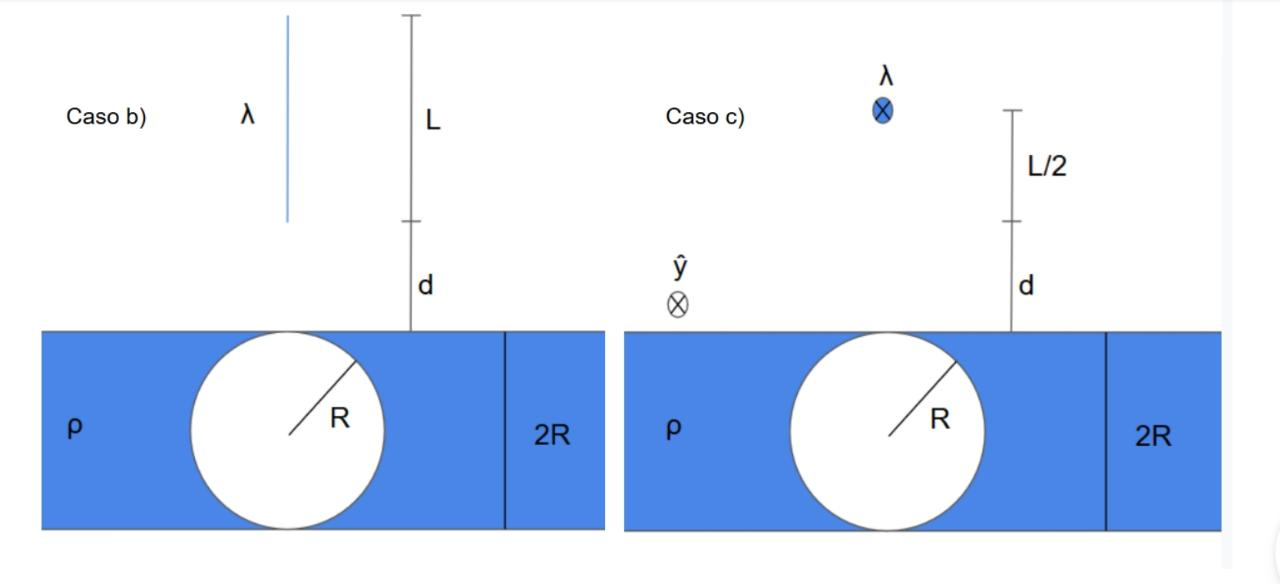
\includegraphics[width=0.9\textwidth]{Electroestática/Campo_electrico/P1 guia2 Mancilla.jpeg}
    \label{fig:P1G2M}
\end{figure}

\np
\begin{enumerate}[label=\alph*)]
    \item Si el campo eléctrico de una carga puntual fuera proporcional a $1/r^3$ en vez de $1/r^2$, ¿seguiría siendo válida la ley de Gauss? Explique su razonamiento. (Sugerencia: considere una superficie esférica centrada en una sola carga puntual).
    \item  Cierta región del espacio limitada por una superficie imaginaria cerrada no contiene carga. ¿El campo eléctrico siempre es igual a cero en todos los puntos de la superficie? Si no es así, ¿en qué circunstancias sería cero en la superficie?
    \item En cierta región del espacio, el campo eléctrico es uniforme. Use la ley de Gauss para demostrar que esa región debe ser eléctricamente neutra; es decir, la densidad volumétrica de carga $\rho$ debe ser igual a cero. Lo contrario, ¿es verdadero? Es decir, en una región del espacio donde no hay carga, ¿debe ser uniforme?
\end{enumerate}

\np
Imagine una esfera de radio R rellena con carga negativa de densidad uniforme y una carga total equivalente a la carga de dos electrones, es decir, $-2e$. En el interior de esta gelatina de carga negativa, se encuentran dos protones, cada uno de ellos de carga $e$. Asuma que, a pesar de la presencia de los protones, la distribución de carga negativa se mantiene uniforme. ¿Dónde deben ubicarse los protones de modo que la fuerza en cada uno de ellos sea nula? Para responder esta pregunta, siga estos pasos:
\begin{enumerate}[label=\alph*)]
    \item Calcule el campo eléctrico producido por los electrones.
    \item Calcule la fuerza de Coulomb neta sobre uno los protones.
    \item Determine la condición de equilibrio y concluya.
\end{enumerate}


\newpage
\subsection{Soluciones}

\sol{1}\newline\newline
$a)$ Al ser metálicas, la esfera y el cascarón son conductores.En equilibrio electrostático, la carga en la superficie interior del cascarón es $-q$ para neutralizar el campo eléctrico de la esfera (que no haya líneas de campo en el conductor) y, dado que su carga total es nula, la carga en la superficie exterior es $q$. Las densidades de carga superficial de la esfera $\sigma_S$, interior del cascarón $\sigma_I$ y exterior del cascarón $\sigma_E$ son uniformes, en el caso de $\sigma_I$ porque la esfera y el cascarón son concéntricos, y están dados por

\[\sigma_S = \frac{q}{4\pi R^2}\]
\[\sigma_I = \frac{-q}{4\pi a^2}\]
\[\sigma_E = \frac{q}{4\pi b^2}\]

$b)$ El espacio está dividido en 4 zonas: al interior de la esfera, $r<R$ (1); entre la esfera y el cascarón, $R<r<a$ (2); interior del cascarón, $a<r<b$ (3); y exterior del cascarón, $b<r$ (4). Como el sistema se compone sólo de conductores y vacío, la densidad volumétrica en todo el espacio es nula. Con esto, utilizando la ecuación de Poisson (calculada en \textbf{\ref{PoissonEsferas}}) el potencial dividido en zonas es

\begin{itemize}
    \item $V_1 = B_1 - \frac{A_1}{r}$
    \item $V_2 = B_2 - \frac{A_2}{r}$
    \item $V_3 = B_3 - \frac{A_3}{r}$
    \item $V_4 = B_4 - \frac{A_4}{r}$
\end{itemize}

Para $r\rightarrow\infty$ el potencial se anula, por lo que $B_4 = 0$, además, dado que en los conductores el potencial es constante, $A_1 = A_3 = 0$.

Los campos eléctricos en (2) y (4) poseen simetría de tipo $\Vec{E}(\Vec{r}) = E(r)\hat{r}$ (demostración en \textbf{\ref{SimetríaEsfera}}), de modo que por ley de Gauss se verifica que

\begin{itemize}
    \item $E_2 = \frac{q}{4\pi\epsilon_o r^2}$
    \item $E_4 = \frac{q}{4\pi\epsilon_o r^2}$
\end{itemize}

Utilizando $\Vec{E} = -\nabla V$ se obtiene

\[\frac{q}{4\pi\epsilon_o r^2} = -\frac{A_2}{r^2} = -\frac{A_4}{r^2}\]

\[A_2 = A_4 = -\frac{q}{4\pi\epsilon_o}\]

Finalmente, por continuidad del potencial

\[V_4(b) = V_3(b) \Rightarrow B_3 = \frac{q}{4\pi\epsilon_o b}\]
\[V_3(a) = V_2(a) \Rightarrow B_2 = \frac{q}{4\pi\epsilon_o}
\left(\frac{1}{b}-\frac{1}{a}\right)\]
\[V_2(R) = V_1(R) \Rightarrow B_1 = \frac{q}{4\pi\epsilon_o}
\left(1+\frac{1}{b}-\frac{1}{a}\right)\]

Se concluye así que

\begin{itemize}
    \item $V_1 = \frac{q}{4\pi\epsilon_o}
\left(1+\frac{1}{b}-\frac{1}{a}\right)$
    \item $V_2 = \frac{q}{4\pi\epsilon_o}\left(
    \frac{1}{r}+\frac{1}{b}-\frac{1}{a}\right)$
    \item $V_3 = \frac{q}{4\pi\epsilon_o b}$
    \item $V_4 = \frac{q}{4\pi\epsilon_o r}$
\end{itemize}
\bigbreak

$c)$ Si se baja el potencial del cascarón a 0, en consecuencia el potencial al exterior de este se anula también

\[V_3 = V_4(b) \Leftrightarrow 0 = -\frac{A_4}{b} \Leftrightarrow A_4 = 0	\Leftrightarrow V_4 = 0\]

Si $V_4 = 0$ entonces $E_4= 0$ y, por ley de Gauss, la carga total encerrada por el cascarón en nula, $\sigma_E = 0$. La carga de la esfera no se ve afectada, de modo que $E_2$ y $A_2$ se mantienen iguales, luego

\[V_2(a) = V_3 \Leftrightarrow B_2 = -\frac{q}{4\pi\epsilon_o a}\]
\[V_2(r) = \frac{q}{4\pi\epsilon_o}\left(\frac{1}{r}
-\frac{1}{a}\right)\]
\[V_1 = V_2(R) = \frac{q}{4\pi\epsilon_o}\left(\frac{1}{R}
-\frac{1}{a}\right)\]

\bigbreak

$d)$ Si $V_3 = V$ entonces

\[V_3 = V_4(b) \Leftrightarrow v = -\frac{A_4}{b} \Leftrightarrow A_4 = -Vb	\Leftrightarrow V_4 = \frac{Vb}{r}\]
\[V_2(a) = V_3 \Leftrightarrow B_2 = V-\frac{q}{4\pi\epsilon_o a}
\Leftrightarrow V_2 = V+\frac{q}{4\pi\epsilon_o}\left(\frac{1}{r}
-\frac{1}{a}\right)\]
\[\Vec{E_4}=-\nabla V_4 = \frac{Vb}{r^2}\hat{r}\]

Para $Q$ la carga total, por ley de Gauss se tiene que

\[E_4= \frac{Q}{4\pi\epsilon_o r^2} = \frac{Vb}{r^2}
\Leftrightarrow Q = 4\pi\epsilon_o Vb\]

Por lo que la carga neta del cascarón es

\[q_c = 4\pi\epsilon_o Vb - q\]

\bigbreak

$e)$ Si se conectan la esfera y el cascarón ambos conformarán un solo conductor y por lo tanto estarán a un mismo potencial. Como la diferencia de potencial es nula, el campo eléctrico en todo el espacio encerrado por el cascarón es 0. Dado que no se produce ningún cambio a la carga total, $E_4$, y por ende $V_4$, son los calculados en $b)$

\[V_1=V_2=V_3=V_4(b)=\frac{q}{4\pi\epsilon_o b}\]
\bigbreak

$f)$ La energía de los conductores desconectados es

\[U_{e1} = \frac{1}{2}(qV_1 + 0\cdot V_3) = \frac{q^2}{8\pi\epsilon_o}
\left(1+\frac{1}{b}-\frac{1}{a}\right)\]

Para los conductores conectados la energía es

\[U_{e2} = \frac{1}{2}qV_3 = \frac{q^2}{8\pi\epsilon_o b}\]

Se tiene $U_{e1} > U_{e2}$ debido a que al conectar los cascarones las cargas se desplazan a causa de un trabajo hecho por el campo, causando que la energía en el sistema disminuya.%para $U_{e1}$ a la energía de los conductores se le agrega la de la interacción entre ambos.

\bigbreak
\bigbreak

\sol{2}\newline\newline
Dado que $L \gg R_1, R_2$ el efecto que tiene cada esfera sobre el potencial de la otra puede ser despreciado. Para $q_1$ y $V_1$ la carga y potencial de la esfera de radio $R_1$, y $q_2$ y $V_2$ la carga y potencial de la esfera de radio $R_2$, se tiene

\[V_1 = \int\frac{\sigma_1}{4\pi\epsilon_o R_1}dS = 
\frac{q_1}{4\pi\epsilon_o R_1}\]

\[V_2 = \frac{q_2}{4\pi\epsilon_o R_2}\]

Como están conectadas, el potencial de las esferas debe ser igual

\[V_1 = V_2 \Leftrightarrow \frac{q_1}{R_1} = \frac{q_2}{R_2}\]

luego

\[Q = q_1 + q_2 = q_1 + \frac{R_2}{R_1}q_1 \Leftrightarrow
q_1 = \frac{R_1 Q}{R_1+R_2}\]

\[q_2 = \frac{R_2 Q}{R_1+R_2}\]

Puesto que $R_1<R_2$, la carga almacenada en la esfera de radio $R_2$ es mayor a la de radio $R_1$

\bigbreak

$b)$ El alambre es parte del conductor por lo que

\[V_{alambre} = V_1 = V_2 = \frac{Q}{4\pi\epsilon_o(R_2+R_1)}\]
\bigbreak

$c)$ La densidad de carga de las esferas es

\[\sigma_1 = \frac{q_1}{4\pi R_1^2} =
\frac{Q}{4\pi R_1(R_1+R_2)}\]
\[\sigma_2 = \frac{q_2}{4\pi R_2^2} =
\frac{Q}{4\pi R_2(R_1+R_2)}\]

Como $R_2 > R_1$, $\sigma_2 < \sigma_1$. El campo eléctrico en las superficies es

\[\Vec{E_1}=\frac{\sigma_1}{\epsilon_o}\hat{r_1}\]
\[\Vec{E_2}=\frac{\sigma_2}{\epsilon_o}\hat{r_2}\]

Donde $\hat{r_i}$ es el vector unitario $\hat{r}$ de las coordenadas esféricas respecto al centro de la esfera de radio $R_i$.
\bigbreak
\bigbreak

\sol{3}\newline\newline
 Usando coordenadas esféricas con origen en el centro de las capas, el espacio se divide en 4 zonas: $r < a$ (1), $a<r<2a$ (2), $2a<r<3a$ (3) y $3a<r$ (4). Las esferas presentan simetría (demostración en \textbf{\ref{SimetríaEsfera}}), por lo que se puede calcular su campo eléctrico con ley de Gauss. Como el sistema comprende sólo conductores y vacío $\rho = 0$ en todo el espacio. De la ecuación de Poisson (resuelta en \ref{PoissonEsferas}) se desprende que en cada zona el potencial es de forma
\[V = B-\frac{A}{r}\]


\begin{enumerate}[label=\alph*)]
    \item Como en (1) no hay carga el campo es nulo
    \[E_1 = 0\]
    \item En (2) la carga encerrada es $Q_{in}$, por lo que el campo eléctrico es
    \[\Vec{E_2} = \frac{Q_{in}}{4\pi\epsilon_o r^2}\hat{r}\]
    \item En (3) la carga encerrada es $Q_{in}+Q$, por lo que el campo eléctrico es
    \[\Vec{E_2} = \frac{Q_{in}+Q}{4\pi\epsilon_o r^2}\hat{r}\]
    \item Para que no haya campo eléctrico al interior del conductor exterior se debe cumplir que $Q_{out} = -(Q+Q_{in})$. Como en el infinito el potencial se anula, en (4) $B=0$ y $V = -\frac{A}{r}$. Igualando $V$ a 0 en $3a$ se obtiene que $A=V=0$ y en concecuencia
    \[E_4 = 0\]


    \item Para $V_2$ el potencial en (2), se verifica que

    \begin{equation}
    \begin{split}
        V_2(r) & = V_2(r) - V_2(a)\\
        & = -\int^r_a\Vec{E_2}\cdot d\Vec{r'}\\
       & = -\int^r_a\frac{Q_{in}}{4\pi\epsilon_o {r'}^2}\,dr'\\
       & = \frac{Q_{in}}{4\pi\epsilon_o r} - \frac{Q_{in}}{4\pi\epsilon_o a}\\
    \end{split}
    \nonumber
    \end{equation}
    Con lo que el potencial en la capa intermedia es

    \[V_2(2a) = -\frac{Q_{in}}{8\pi\epsilon_o a}\]
    \medbreak
    Para $V_3$ el potencial en (3), se verifica que

    \begin{equation}
    \begin{split}
      V_3(r) & = V_3(r) - V_3(3a)\\
      & = -\int^r_{3a}\Vec{E_3}\cdot d\Vec{r'}\\
      & = -\int^r_{3a}\frac{Q_{in}+Q}{4\pi\epsilon_o {r'}^2}\,dr'\\
      & = \frac{Q_{in}+Q}{4\pi\epsilon_o r} - \frac{Q_{in}+Q}{12\pi\epsilon_o a}\\
    \end{split}
    \nonumber
    \end{equation}
    Con lo que el potencial en la capa intermedia es

    \[V_3(2a) = \frac{Q_{in}+Q}{24\pi\epsilon_o a}\]
    \medbreak
    \item Como $V_2(2a)=V_3(2a)$, se tiene que

    \[\frac{Q_{in}+Q}{24\pi\epsilon_o a} = -\frac{Q_{in}}{8\pi\epsilon_o a}\]
    \[\implies Q_{in}=-\frac{1}{4}Q\]
    
    \medbreak
    \item Puesto que las capas exterior e interior están a igual potencial se las puede tomar como un solo conductor de carga $Q_{in} + Q_{out} = -Q$, formando un condensador con la capa intermedia. La capacitancia del sistema está dada por
    
    
    \[C = \frac{Q}{\Delta V} = 32\pi\epsilon_o a\]
    
    Esto también se puede ver como si se tuvieran dos condensadores en paralelo, uno con carga $Q_{in}$ y otro con carga $Q_{out}$ y misma diferencia de potencial $V(2a)$. Al estar en paralelos su capacitancia equivalente sería la suma de las capacitancias individuales, dando el resultado anterior.
    
    La razón de que pueden verse como condensadores en paralelo yace en que poseen el mismo potencial en ambos extremos, en uno están a potencial $V=0$ y en el otro a potencial $V = V(2a)$. En la siguiente imagen se visualiza de manera circuital
    
    \begin{figure}[H]
        \centering
        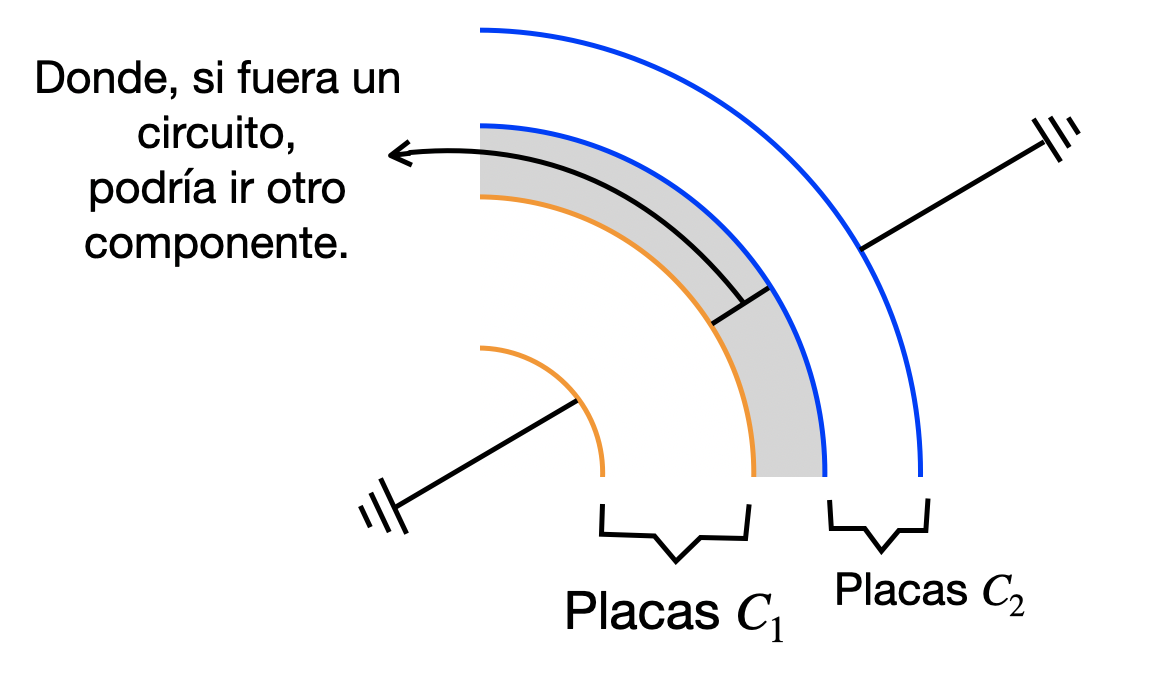
\includegraphics[width=0.5\textwidth]{Electroestática/conductores/P3IG.png}
    \end{figure}
    
    En la figura anterior el conductor de radio $a$ es el inferior izquierdo, el conductor de radio $2a$ está representado por el conductor 'con anchura' de color gris, y el conductor de radio $3a$ es el superior derecho. Las conexiones con 3 líneas representan conexiones a tierra. Y los condensadores son representados el primero con color amarillo-naranjo y el segundo con color azul. 
    
    \medbreak
    \item El sistema está compuesto por 3 conductores y 2 condensadores, como las capas interna y externa tienen potencial nulo, la energía queda dada sólo por la capa intermedia

    \[U_e = \frac{1}{2}V_2(2a) = \frac{1}{8}\frac{Q^2}{8\pi\epsilon_o a}\]
    
    Esto es equivalente a calcular la capacitancia de un condensador equivalente y, haciendo uso de $V(2a)$, obtener la energía potencial con
    $U_e = \frac{1}{2}C\Delta V^2$. 

\end{enumerate}
\bigbreak
\bigbreak
\sol{4}\newline
% Podriamos especificar la alineación de las placas y agregar imagen

\begin{enumerate}[label=\alph*)]
    %a
    \item Como las dimensiones laterales de las placas son mucho más grandes que $x$, se puede aproximar el campo eléctrico de una de las placas al de un plano infinito

    \[\Vec{E} = \frac{Q}{2A\epsilon_o}\hat{x}\]

    ubicando el origen en la placa de carga $Q$, el trabajo par desplazar la placa de carga $-Q$ en $\Delta x$ es

    \begin{equation}
        \begin{split}
            W_{ext} &= Q\int^{x+\Delta x}_x \Vec{E}\cdot d\Vec{r}\\
            & = Q\int^{x+\Delta x}_x\frac{Q}{2A\epsilon_o}\,dr\\
            & = \frac{Q^2}{2A\epsilon_o}\Delta x\\
        \end{split}
        \nonumber
    \end{equation}
    \medbreak
%b
    \item Por teorema de trabajo-energía, se cumple que la diferencia de energía potencial es igual al trabajo hecho por la fuerza externa, por lo que

    \[\Delta U_e = W = \frac{Q^2}{2A\epsilon_o}\Delta x\]
    Notemos que al ser el trabajo positivo, la fuerza externa está inyectando energía al sistema, por lo que se tiene que no se conserva la energía del sistema al aumentar la separación entre las placas por un $\Delta x$
    
    La energía potencial del sistema también se puede calcular haciendo uso del condensador, donde $U_e = \frac{1}{2}Q\Delta V = \frac{Q^2}{2C}$. Como se tiene que la carga de las placas no cambia, entonces se tiene que $C$ y $\Delta V$ han de cambiar. En específico, como se separan las placas $C$ pasa a ser $\frac{\epsilon_o A}{x+\Delta x}$ (calculado en \ref{C:placas}).
%c Aux_5 Daniela Mancilla Otoño 2020
    \item Siguiendo la idea del párrafo anterior, si es que al realizar trabajo cambia la energía del sistema, lo que implica un cambio en el condensador, (carga o diferencia de potencial) entonces al mantener la batería conectada se mantendrá la diferencia de potencial igual. Con esto en mente, entonces será necesario que la carga del condensador cambie.
    
    \begin{equation}
    \begin{split}
        W_{ext} &= \int^{x+\Delta x}_x Q\Vec{E}\cdot d\Vec{r}\\
        & = \int^{x+\Delta x}_x \frac{Q^2}{2A\epsilon_o}\,dr\\
        & = \int^{x+\Delta x}_x
        \frac{(CV_o)^2}{2A\epsilon_o}\,dr\\
        & = \int^{x+\Delta x}_x
        \frac{\epsilon_o AV_o^2}{2r^2}\,dr\\
        &=\frac{\epsilon_o AV_o^2}{2}\left(
        -\frac{1}{x+\Delta x}+\frac{1}{x}\right)\\
        &=\frac{\epsilon_o AV_o^2\Delta x}{2x(x+\Delta x)}
    \end{split}
    \nonumber
    \end{equation} 
    
    \medbreak

%d
    \item La energía potencial eléctrica inicial es
    
    \[U_i = \frac{1}{2}C_iV_o^2 = \frac{\epsilon_o A}{2x}V_o^2\]
    
    la energía potencial final es
    
    \[U_f = \frac{1}{2}C_fV_o^2 = 
    \frac{\epsilon_o A}{2(x+\Delta x)}V_o^2\]
    
    de modo que
    
    \[\Delta U = U_f-U_i = -\frac{\epsilon_o AV_o^2\Delta x}{2x(x+\Delta x)}\]
    
    % Hay que mostrar que la energía que se conserva

\end{enumerate}

\bigbreak
\bigbreak

\sol{5}\newline

\begin{enumerate}[label=\alph*)]
    \item El campo eléctrico en todo el espacio puede ser obtenido haciendo uso de la Ley de Gauss y de la definición de campo eléctrico, debido a lo que será pedido en los siguientes incisos solo será calculado en el caso $\rho > a$ y $\abs{z} < L/2$. Donde se están usando coordenadas cilíndricas y el centro del cilindro como eje.\\
    
    Partamos calculando la densidad superficial de carga, la densidad de carga es superficial a causa de que estamos frente a un conductor que no puede tener campo eléctrico interno, con esto tenemos que 
    \[\sigma = \frac{Q}{2\pi aL}\]
    A causa de que está solo en el manto y el área del manto es $2\pi aL$.\\
    
    Haciendo uso de la Ley de Gauss y sabiendo que por simetría (\ref{SimetríaCilindrosInf}) hay solo campo en la dirección $\hat{\rho}$, establecemos un cilindro más grande superpuesto con el original, de radio $\rho$ y altura $h$, con esto
    %no tiene que ser infinito?, no también el largo(altura) puede ser mucha mayor al radio
    \begin{equation}
        \begin{split}
            &\oint_{Manto} \Vec{E}\cdot d\Vec{S} = \frac{Q_{enc}}{\epsilon_0}\\
            \implies &\int E(\rho)dS = \frac{\sigma 2\pi a h}{\epsilon_0}\\
            \implies &E(\rho) \int dS = \frac{\sigma 2\pi a h}{\epsilon_0}\\
            \implies &E(\rho) 2 \pi \rho h = \frac{\sigma 2\pi a h}{\epsilon_0}\\
            \implies &E(\rho) = \frac{\sigma a}{\epsilon_0 \rho}\\
            \therefore \quad &\Vec{E}(\rho) = \frac{\sigma a}{\epsilon_0 \rho}\hat{\rho}
        \end{split}
        \nonumber 
    \end{equation}
    
    \item Sea $\sigma_+$ la densidad superficial del manto del cilindro de radio $a_1$ y $\sigma_-$ la densidad superficial del manto del cilindro de radio $a_2$, tenemos que el campo eléctrico de cada cilindro será
    
    \[\Vec{E}_{a_1} = \frac{\sigma_+ a_1}{\epsilon_0 \rho}\hat{\rho}\]
    \[\Vec{E}_{a_2} = \frac{\sigma_- a_2}{\epsilon_0 \rho}\hat{\rho'}\]
    
    Si calculamos el campo en $P$ debemos sumar ambos campos, y se tiene que $\hat{\rho'} = - \hat{\rho}$, ya que están centrados en distintos ejes los campos, y en $P$ las direcciones son justo contrarias, así
    
    \[\Vec{E}_{\text{en P}} = \left( \frac{\sigma_+ a_1}{\epsilon_0 r} - \frac{\sigma_- a_2}{\epsilon_0 (d-r)} \right)\hat{\rho}\]
    
    \item Para calcular la diferencia de potencial calculamos $V(a_1) - V(d - a_2)$ por definición,
    
    \begin{equation}
        \begin{split}
            V(a_1) - V(d - a_2) &= -\int_{d-a_2}^{a_1}\left[ \frac{\sigma_+ a_1}{\epsilon_0 r} - \frac{\sigma_- a_2}{\epsilon_0 (d-r)} \right]dr\\
            &= -\left.\left[ \frac{\sigma_+ a_1}{\epsilon_0}\ln{(r)} + \frac{\sigma_- a_2}{\epsilon_0}\ln{(d-r)} \right]\right\rvert_{d-a_2}^{a_1}\\
            &\vdots \quad\\ 
            &\approx -\left[ \frac{\sigma_+}{\epsilon_0}a_1\ln{\left( \frac{a_1}{d} \right)} - \frac{\sigma_-}{\epsilon_0}a_2\ln{\left( \frac{a_2}{d} \right)} \right]\\
            \text{Donde en } \vdots \text{ se usó que } &d-a_1 \approx d\text{ y } d-a_2 \approx d\text{, al ser }d \gg a_1\text{ y } d \gg a_2\\
        \end{split}
        \nonumber
    \end{equation}
    
    Reemplazamos $\sigma_+ = Q/(2\pi La_1)$ y $\sigma_- = -Q/(2\pi La_2)$, y nos queda
    
    \begin{equation}
        \begin{split}
            \Delta V &= -\left[ \frac{Q}{2 \pi L\epsilon_0}\ln{\left( \frac{a_1}{d} \right)} + \frac{Q}{2 \pi L\epsilon_0}\ln{\left( \frac{a_2}{d} \right)} \right]\\
            &=\frac{Q}{2 \pi L \epsilon_0}\ln{\left( \frac{d^2}{a_1a_2} \right)}\\
            &=\frac{Q}{\pi L \epsilon_0}\ln{\left( \frac{d}{\sqrt{a_1a_2}} \right)}
        \end{split}
        \nonumber
    \end{equation}
    
    Lo que nos da que la capacitancia del sistema es
    \[C_{tot} \approx \frac{Q}{\Delta V} = \frac{\pi \epsilon_0 L}{\ln{\left( \frac{d}{\sqrt{a_1a_2}} \right)}}\]
    
    \item Como se tiene que nos piden la capacitancia por unidad de largo debemos dividir la capacitancia encontrada por $L$, así
    \[C \approx \frac{\pi \epsilon_0}{\ln{\left( \frac{d}{\sqrt{a_1a_2}} \right)}}\]
    
    \item Está situación es similar a la presentada en el problema 7.2, por lo que las cargas se distribuirían a través de los cilindros dependiendo de las razones entre sus radios, y el potencial se volvería el mismo para ambos.
    
\end{enumerate}

\sol{6}\newline

\begin{enumerate}[label=\alph*)]
    \item Digamos que la capa del radio interno tiene una carga $-Q$ en su cara exterior, y la capa externa una carga $Q$ en su cara interior. Así queda la configuración como en la siguiente imagen
    \begin{figure}[H]
        \centering
        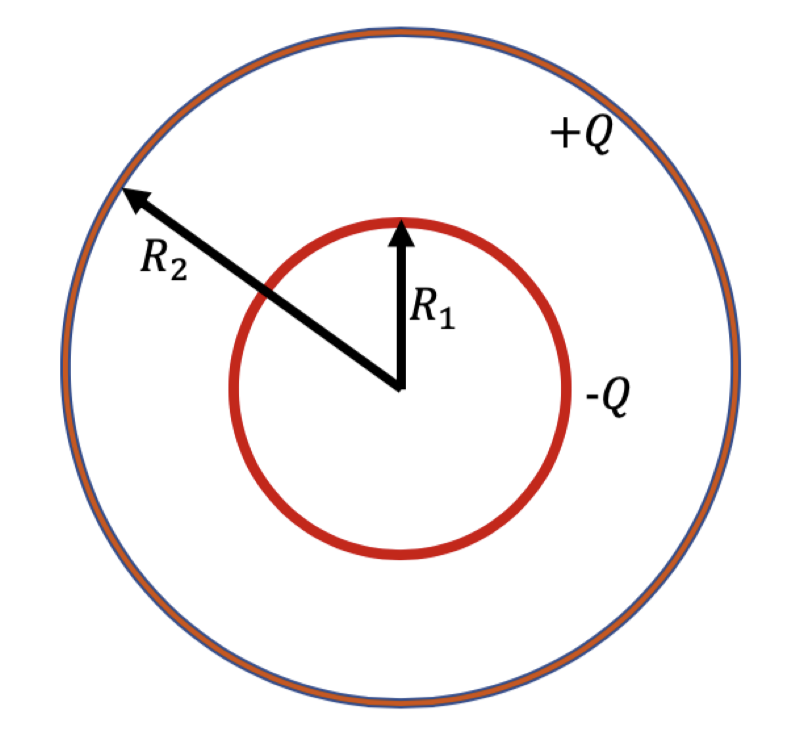
\includegraphics[width=0.47\textwidth]{Electroestática/conductores/P6IA.png}
        \label{fig:sol_6_conduc}
    \end{figure}
    
    Para calcular la capacitancia calculemos la diferencia de potencial entre ambas caras, para esto calculemos el campo eléctrico e integramos de $R_1$ a $R_2$.\\
    
    Usando Ley de Gauss y una superficie Gaussiana de largo $L$ y radio $\rho$, con $R_1 < \rho < R_2$,
    \[\oint_{Manto} \Vec{E}\cdot d\Vec{S} = \frac{Q_{enc}}{\epsilon_0}\]
    \[\implies E(\rho) = \frac{-Q}{2 \pi L \epsilon_0 \rho}\]
    Ahora calculamos la diferencia de potencial,
    \[\Delta V = V(R_2) - V(R_1) =-\int_{R_1}^{R_2}\frac{-Q}{2 \pi L \epsilon_0 \rho}d\rho = \frac{Q}{2\pi L \epsilon_0}\ln{\left( \frac{R_2}{R_1} \right)}\]
    Ahora usando $C = Q/\Delta V$ podemos obtener la capacitancia del sistema
    \[C = \frac{Q}{\Delta V} = \frac{2\pi L \epsilon_0}{\ln{\left( \frac{R_2}{R_1} \right)}}\]
    \text{ }\\     
    % Problema 2 Aux 5 D. Mancilla Otoño2020 (Pauta en Ucursos)
    
    \item \textbf{(Sin valores actualmente)} El nuevo condensador es como el mostrado a continuación
    \begin{figure}[H]
        \centering
        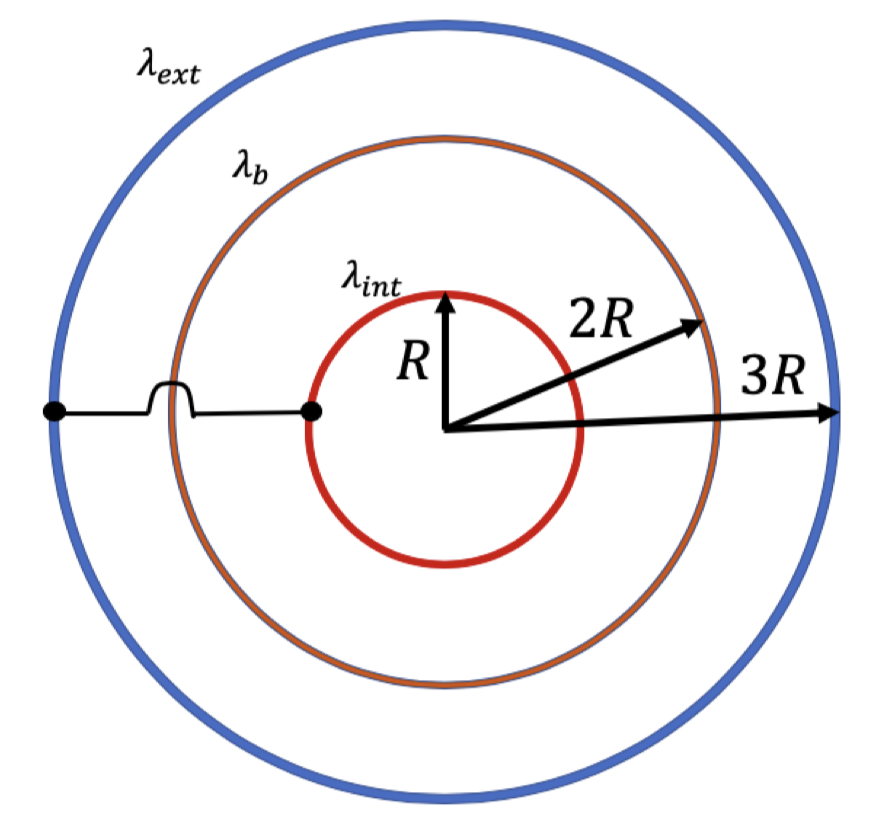
\includegraphics[width=0.47\textwidth]{Electroestática/conductores/P6IB.png}
    \end{figure}
    % Completar respuestas con desarrollo y resultados
    Como se tiene que la capa de radio $R$ y la de radio $3R$ están conectadas entonces sus potenciales son iguales, sabiendo esto y con la Ley de Gauss se puede calcular el campo eléctrico y obtener expresiones para los voltajes. Y usando $V(R) - V(2R) = V(3R) - V(2R)$ se puede despejar $\lambda_{int}$. Luego usando que son conductores y comienzan neutrales se tiene $0 = \lambda_{ext} + \lambda_{int} + \lambda_b$, y se puede obtener el valor de $\lambda_{ext}$
    % Completar respuestas con desarrollo y resultados    
    \item Para despejar la capacitancia se ocupa la relación entre energía potencial eléctrica y capacitancia, y además se despeja usando la definición que la relaciona con el voltaje.
    % (Copiado del aux)
    \item Las cargas ($\lambda_{int}, \lambda_{ext} $ y $ \lambda_b$) permanecen donde se encontraban. Con respecto a $\lambda_{nuevo}$, se distribuirá de manera uniforme en la superficie exterior ($r=3R$).
    
    
\end{enumerate}
\newpage


% Campo Magnético
\section{Campo Magnético}

Una carga puntual $q$ con posición $\Vec{r}_q$ que se desplaza con velocidad $\Vec{v}_q$, produce un campo magnético dado por

\[\Vec{B}(\Vec{r})=\frac{\mu_o}{4\pi}
\frac{q\Vec{v}_q\times(\Vec{r}-\Vec{r}_q)}{\|\Vec{r}-\Vec{r}_q\|^3}\]

donde la permeabilidad del vacío, $\mu_o$, es una constante que verifica $\frac{1}{\epsilon_o\mu_o}=c$, con $c$ la velocidad de la luz.

\subsection{Ley de Biot-Savart}

Para una distribución de cargas continua, el campo magnético es

\[\Vec{B}=\frac{\mu_o}{4\pi}\int\Vec{J}(\Vec{r}_q)\times
\frac{(\Vec{r}-\Vec{r}_q)}{\|\Vec{r}-\Vec{r}_q\|^3}\,d\V_q\]\\
% La ecuación de arriba es la Ley de Biot-Savart
si bien $d\V_q$ es un diferencial de volumen, la definición es también válida para distribuciones superficiales ($d\Vec{S}_q$) y lineales ($d\Vec{r}_q$). Para casos superficiales la densidad de corriente se suele escribir como $\Vec{K} = \sigma \vec{v}$ y en lineales se usa la intensidad con su dirección ($\Vec{I}dr = Id\Vec{r}$).

\subsection{Ecuaciones de Maxwell}

La tercera y cuarta ecuación de Maxwell se aplican en magnetoestática, y son

\begin{equation}
\begin{split}
   \nabla\cdot \Vec{B} &= 0\\
    \nabla \times \Vec{B} &= \mu_0\Vec{J}
\end{split}
\nonumber
\end{equation}

La forma integral de la primera ecuación es
\[ \oint\Vec{B}\cdot d\vec{s} = 0 \]

\subsubsection{Ley de Ampere}

La forma integral de la segunda ecuación se conoce como la Ley de Ámpere, esta es

\[ \oint \vec{B}\cdot d\vec{l} = \mu_0\int \vec{J}\cdot d\vec{s} \]

Para una superficie regular orientable $\Lambda$, con borde $\partial\Gamma$, se cumple que

\[\oint_{\partial\Lambda}\vec{B}\cdot d\vec{l} = \mu_0\int_\Lambda \vec{J}\cdot d\vec{s} = \mu_0I_{\text{enc}}\]

donde $I_{\text{enc}}$ es la intensidad de corriente que pasa por $\Lambda$. Dado que $I$ no se anula (en tal caso no existiría $\vec{B}$), se concluye que las lineas de campo magnético son siempre cerradas, en concreto, se cierran en torno a la corriente.\\

Bajo condiciones de simetría, simlilar a como sucede con la ley de Gauss, se puede usar la ley de Ampere para determinar el campo magnético, en sólo ciertas configuraciones (o figuras geométricas), como:
\begin{itemize}
    \item Líneas rectas infinitas
    \item Planos infinitos
    \item Solenoides infinitos 
    
    
    (también visualizable como un cilindro con corriente superficial con dirección en $\hat \phi$)
    \item Toroides
\end{itemize}


\subsection{Fuerza Magnética}

Un campo magnético $\Vec{B}$ produce sobre una carga puntual $q$ en movimiento, con velocidad $\Vec{v}$, una fuerza dada por

\[\Vec{F}_m=q\Vec{v}\times\Vec{B}\]
\bigbreak
Para una distribución de cargas continua, la fuerza magnética es

\[\Vec{F}_m=\int\Vec{J}\times\Vec{B}\,d\V\]

Al igual que como pasa con $\Vec{B}$, $d\V$ puede reemplazarse por $d\Vec{S}$ o $d\Vec{r}$.\\

La fuerza magnética \textbf{no} realiza trabajo sobre una partícula.
% El trabajo realizado por la fuerza magnética sobre una partícula es siempre cero.


\subsection{Fuerza de Lorentz}

Se denomina fuerza de Lorentz a la fuerza eléctrica total

\[\Vec{F}=q\Vec{E}+q\Vec{v}\times\Vec{B}\]

\subsection{Potencial Vectorial}

Se define el vector

\[\Vec{A}=\frac{\mu_o}{4\pi}\int\frac{\Vec{J}(\Vec{r}_q)}{\|\Vec{r}-\Vec{r}_q\|}\,d\V_q\]

$\Vec{A}$ es un potencial vectorial de $\Vec{B}$, puesto que se verifica que

\[\Vec{B}=\nabla\times\Vec{A}\]

% Cordero define A ligeramente distinto, pero me da pereza revisar las justificaciones

\subsection{Dipolo Magnético}

Para una espira por la que fluye corriente eléctrica, se define el momento dipolar magnético como

\[\Vec{m}=I\Vec{S}\]

Para distribuciones continuas se tiene

\begin{eqit}
    &\Vec{m}_l = \frac{I}{2}\oint\Vec{r}\times d\Vec{r}\\
    &\Vec{m}_S = \frac{1}{2}\int\Vec{r}\times \Vec{K}\,dS\\
    &\Vec{m}_V = \frac{1}{2}\int\Vec{r}\times \Vec{J}\,d\V\\
\end{eqit}\\

A grandes distancias se verifica que

\begin{eqit}
    &\Vec{A} = \frac{\mu_o}{4\pi}
    \frac{\Vec{m}\times\Vec{r}}{r^3}\\
    &\Vec{B}=\frac{\mu_o}{4\pi}\frac{3\lados{(}{\Vec{m}\cdot
    \Vec{r}}\Vec{r}-r^2\Vec{m}}{r^5}\\
\end{eqit}\\

Para una espira lo suficientemente pequeña, la fuerza magnética y el torque sobre el dipolo son

\begin{eqit}
    &\Vec{F} = \nabla\lados{(}{\Vec{m}\cdot\Vec{B}_{ext}}\\
    &\Vec{\tau} = \Vec{m}\times\Vec{B}_{ext}\\
\end{eqit}

\newpage
\subsection{Problemas}
--------------------------------------------------------
\\

\np
Dos varillas de longitud $L$ están a lo largo del eje $x$, una entre $x=a/2$ y $x=a/2+L$ y la otra entre $x=-a/2$ y $x=-a/2-L$. Cada varilla tiene carga positiva Q distribuida uniformemente.

\begin{enumerate}[label=\alph*)]
    \item Calcule el campo eléctrico producido por la segunda varilla en puntos a lo largo del eje $x$ positivo.
    \item Calcule la magnitud de la fuerza que ejerce una varilla sobre la otra.
\end{enumerate}

\np
\begin{enumerate}[label=\alph*)]
    \item Determine el campo eléctrico en todos los puntos del eje de un anillo de radio $R$ sobre el cual hay una densidad de carga uniforme $\lambda$.
    \item A partir de su resultado anterior, calcule el campo eléctrico creado por una corona circular de radios $R_1$ y $R_2$ ($R_1 < R_2$), sobre la cual hay una densidad de carga uniforme $\sigma$, en los puntos de su eje. Encuentre la magnitud y la dirección del campo eléctrico. Considere puntos arriba y abajo de la corona circular.
    \item ¿A qué se reduce su resultado si $R_1 \longrightarrow 0$? ¿Y si $R_2 \longrightarrow \infty$?
    \item Demuestre que en puntos sobre el eje de la corona (eje $z$) que estén suficientemente cerca del origen, la magnitud del campo eléctrico es aproximadamente proporcional a la distancia entre el centro de la corona circular y el punto. ¿Qué tan cerca es ”suficientemente cerca”?
\end{enumerate}

\np
\begin{enumerate}[label=\alph*)]
    \item Encuentre el campo eléctrico creado por un segmento rectilíneo de longitud $L$ dotado de una densidad de carga uniforme $\lambda$.
    \item A partir del resultado anterior, calcule el campo eléctrico en todos los puntos del espacio, producido por una línea infinita con densidad de carga $\lambda$.
    \item Calcule el flujo de campo eléctrico a través de una superficie cilíndrica cerrada, de largo h y radio R, concéntrica con la línea infinita.
    \item  Se tienen dos líneas infinitas con densidad de carga $\lambda$ y $-\lambda$, situadas a una distancia $2a$ una de la otra. Encuentre la fuerza por unidad de longitud que se establece entre los dos hilos. ¿Es atractiva o repulsiva?
\end{enumerate}
\newpage
\np
Considere un plano infinito (en las direcciones $x$ e $y$) de grosor $2R$ (en la dirección $z$), cargado con una densidad de carga volumétrica $\rho$ uniforme. Este plano tiene un agujero cilíndrico (cuyo eje coincide con el eje $y$) de radio $R$ sin cargas.
\begin{enumerate}[label=\alph*)]
    \item Determine el campo eléctrico en todo el espacio. Note que debería dividir el resultado en 3 zonas distintas.
    \item Calcule la fuerza que experimenta un alambre de largo $L$ con densidad de carga lineal uniforme $\lambda$ ubicado a una distancia $d$ del plano y extendido en la dirección $z$.
    \item Calcule la fuerza que experimenta un alambre de largo $L$ con densidad de carga lineal uniforme $\lambda$ ubicado a una distancia $d+L/2$ del plano y extendido en la dirección $y$.
\end{enumerate}

\begin{figure}[h]
    \centering
    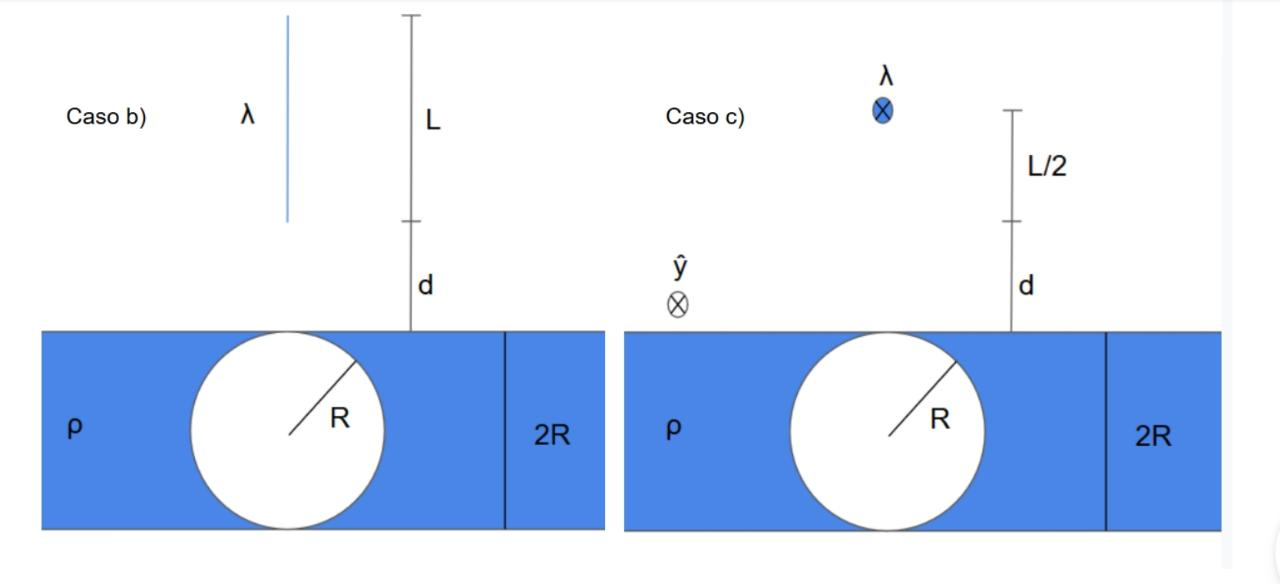
\includegraphics[width=0.9\textwidth]{Electroestática/Campo_electrico/P1 guia2 Mancilla.jpeg}
    \label{fig:P1G2M}
\end{figure}

\np
\begin{enumerate}[label=\alph*)]
    \item Si el campo eléctrico de una carga puntual fuera proporcional a $1/r^3$ en vez de $1/r^2$, ¿seguiría siendo válida la ley de Gauss? Explique su razonamiento. (Sugerencia: considere una superficie esférica centrada en una sola carga puntual).
    \item  Cierta región del espacio limitada por una superficie imaginaria cerrada no contiene carga. ¿El campo eléctrico siempre es igual a cero en todos los puntos de la superficie? Si no es así, ¿en qué circunstancias sería cero en la superficie?
    \item En cierta región del espacio, el campo eléctrico es uniforme. Use la ley de Gauss para demostrar que esa región debe ser eléctricamente neutra; es decir, la densidad volumétrica de carga $\rho$ debe ser igual a cero. Lo contrario, ¿es verdadero? Es decir, en una región del espacio donde no hay carga, ¿debe ser uniforme?
\end{enumerate}

\np
Imagine una esfera de radio R rellena con carga negativa de densidad uniforme y una carga total equivalente a la carga de dos electrones, es decir, $-2e$. En el interior de esta gelatina de carga negativa, se encuentran dos protones, cada uno de ellos de carga $e$. Asuma que, a pesar de la presencia de los protones, la distribución de carga negativa se mantiene uniforme. ¿Dónde deben ubicarse los protones de modo que la fuerza en cada uno de ellos sea nula? Para responder esta pregunta, siga estos pasos:
\begin{enumerate}[label=\alph*)]
    \item Calcule el campo eléctrico producido por los electrones.
    \item Calcule la fuerza de Coulomb neta sobre uno los protones.
    \item Determine la condición de equilibrio y concluya.
\end{enumerate}


\newpage
\subsection{Soluciones}

\sol{1}\newline\newline
$a)$ Al ser metálicas, la esfera y el cascarón son conductores.En equilibrio electrostático, la carga en la superficie interior del cascarón es $-q$ para neutralizar el campo eléctrico de la esfera (que no haya líneas de campo en el conductor) y, dado que su carga total es nula, la carga en la superficie exterior es $q$. Las densidades de carga superficial de la esfera $\sigma_S$, interior del cascarón $\sigma_I$ y exterior del cascarón $\sigma_E$ son uniformes, en el caso de $\sigma_I$ porque la esfera y el cascarón son concéntricos, y están dados por

\[\sigma_S = \frac{q}{4\pi R^2}\]
\[\sigma_I = \frac{-q}{4\pi a^2}\]
\[\sigma_E = \frac{q}{4\pi b^2}\]

$b)$ El espacio está dividido en 4 zonas: al interior de la esfera, $r<R$ (1); entre la esfera y el cascarón, $R<r<a$ (2); interior del cascarón, $a<r<b$ (3); y exterior del cascarón, $b<r$ (4). Como el sistema se compone sólo de conductores y vacío, la densidad volumétrica en todo el espacio es nula. Con esto, utilizando la ecuación de Poisson (calculada en \textbf{\ref{PoissonEsferas}}) el potencial dividido en zonas es

\begin{itemize}
    \item $V_1 = B_1 - \frac{A_1}{r}$
    \item $V_2 = B_2 - \frac{A_2}{r}$
    \item $V_3 = B_3 - \frac{A_3}{r}$
    \item $V_4 = B_4 - \frac{A_4}{r}$
\end{itemize}

Para $r\rightarrow\infty$ el potencial se anula, por lo que $B_4 = 0$, además, dado que en los conductores el potencial es constante, $A_1 = A_3 = 0$.

Los campos eléctricos en (2) y (4) poseen simetría de tipo $\Vec{E}(\Vec{r}) = E(r)\hat{r}$ (demostración en \textbf{\ref{SimetríaEsfera}}), de modo que por ley de Gauss se verifica que

\begin{itemize}
    \item $E_2 = \frac{q}{4\pi\epsilon_o r^2}$
    \item $E_4 = \frac{q}{4\pi\epsilon_o r^2}$
\end{itemize}

Utilizando $\Vec{E} = -\nabla V$ se obtiene

\[\frac{q}{4\pi\epsilon_o r^2} = -\frac{A_2}{r^2} = -\frac{A_4}{r^2}\]

\[A_2 = A_4 = -\frac{q}{4\pi\epsilon_o}\]

Finalmente, por continuidad del potencial

\[V_4(b) = V_3(b) \Rightarrow B_3 = \frac{q}{4\pi\epsilon_o b}\]
\[V_3(a) = V_2(a) \Rightarrow B_2 = \frac{q}{4\pi\epsilon_o}
\left(\frac{1}{b}-\frac{1}{a}\right)\]
\[V_2(R) = V_1(R) \Rightarrow B_1 = \frac{q}{4\pi\epsilon_o}
\left(1+\frac{1}{b}-\frac{1}{a}\right)\]

Se concluye así que

\begin{itemize}
    \item $V_1 = \frac{q}{4\pi\epsilon_o}
\left(1+\frac{1}{b}-\frac{1}{a}\right)$
    \item $V_2 = \frac{q}{4\pi\epsilon_o}\left(
    \frac{1}{r}+\frac{1}{b}-\frac{1}{a}\right)$
    \item $V_3 = \frac{q}{4\pi\epsilon_o b}$
    \item $V_4 = \frac{q}{4\pi\epsilon_o r}$
\end{itemize}
\bigbreak

$c)$ Si se baja el potencial del cascarón a 0, en consecuencia el potencial al exterior de este se anula también

\[V_3 = V_4(b) \Leftrightarrow 0 = -\frac{A_4}{b} \Leftrightarrow A_4 = 0	\Leftrightarrow V_4 = 0\]

Si $V_4 = 0$ entonces $E_4= 0$ y, por ley de Gauss, la carga total encerrada por el cascarón en nula, $\sigma_E = 0$. La carga de la esfera no se ve afectada, de modo que $E_2$ y $A_2$ se mantienen iguales, luego

\[V_2(a) = V_3 \Leftrightarrow B_2 = -\frac{q}{4\pi\epsilon_o a}\]
\[V_2(r) = \frac{q}{4\pi\epsilon_o}\left(\frac{1}{r}
-\frac{1}{a}\right)\]
\[V_1 = V_2(R) = \frac{q}{4\pi\epsilon_o}\left(\frac{1}{R}
-\frac{1}{a}\right)\]

\bigbreak

$d)$ Si $V_3 = V$ entonces

\[V_3 = V_4(b) \Leftrightarrow v = -\frac{A_4}{b} \Leftrightarrow A_4 = -Vb	\Leftrightarrow V_4 = \frac{Vb}{r}\]
\[V_2(a) = V_3 \Leftrightarrow B_2 = V-\frac{q}{4\pi\epsilon_o a}
\Leftrightarrow V_2 = V+\frac{q}{4\pi\epsilon_o}\left(\frac{1}{r}
-\frac{1}{a}\right)\]
\[\Vec{E_4}=-\nabla V_4 = \frac{Vb}{r^2}\hat{r}\]

Para $Q$ la carga total, por ley de Gauss se tiene que

\[E_4= \frac{Q}{4\pi\epsilon_o r^2} = \frac{Vb}{r^2}
\Leftrightarrow Q = 4\pi\epsilon_o Vb\]

Por lo que la carga neta del cascarón es

\[q_c = 4\pi\epsilon_o Vb - q\]

\bigbreak

$e)$ Si se conectan la esfera y el cascarón ambos conformarán un solo conductor y por lo tanto estarán a un mismo potencial. Como la diferencia de potencial es nula, el campo eléctrico en todo el espacio encerrado por el cascarón es 0. Dado que no se produce ningún cambio a la carga total, $E_4$, y por ende $V_4$, son los calculados en $b)$

\[V_1=V_2=V_3=V_4(b)=\frac{q}{4\pi\epsilon_o b}\]
\bigbreak

$f)$ La energía de los conductores desconectados es

\[U_{e1} = \frac{1}{2}(qV_1 + 0\cdot V_3) = \frac{q^2}{8\pi\epsilon_o}
\left(1+\frac{1}{b}-\frac{1}{a}\right)\]

Para los conductores conectados la energía es

\[U_{e2} = \frac{1}{2}qV_3 = \frac{q^2}{8\pi\epsilon_o b}\]

Se tiene $U_{e1} > U_{e2}$ debido a que al conectar los cascarones las cargas se desplazan a causa de un trabajo hecho por el campo, causando que la energía en el sistema disminuya.%para $U_{e1}$ a la energía de los conductores se le agrega la de la interacción entre ambos.

\bigbreak
\bigbreak

\sol{2}\newline\newline
Dado que $L \gg R_1, R_2$ el efecto que tiene cada esfera sobre el potencial de la otra puede ser despreciado. Para $q_1$ y $V_1$ la carga y potencial de la esfera de radio $R_1$, y $q_2$ y $V_2$ la carga y potencial de la esfera de radio $R_2$, se tiene

\[V_1 = \int\frac{\sigma_1}{4\pi\epsilon_o R_1}dS = 
\frac{q_1}{4\pi\epsilon_o R_1}\]

\[V_2 = \frac{q_2}{4\pi\epsilon_o R_2}\]

Como están conectadas, el potencial de las esferas debe ser igual

\[V_1 = V_2 \Leftrightarrow \frac{q_1}{R_1} = \frac{q_2}{R_2}\]

luego

\[Q = q_1 + q_2 = q_1 + \frac{R_2}{R_1}q_1 \Leftrightarrow
q_1 = \frac{R_1 Q}{R_1+R_2}\]

\[q_2 = \frac{R_2 Q}{R_1+R_2}\]

Puesto que $R_1<R_2$, la carga almacenada en la esfera de radio $R_2$ es mayor a la de radio $R_1$

\bigbreak

$b)$ El alambre es parte del conductor por lo que

\[V_{alambre} = V_1 = V_2 = \frac{Q}{4\pi\epsilon_o(R_2+R_1)}\]
\bigbreak

$c)$ La densidad de carga de las esferas es

\[\sigma_1 = \frac{q_1}{4\pi R_1^2} =
\frac{Q}{4\pi R_1(R_1+R_2)}\]
\[\sigma_2 = \frac{q_2}{4\pi R_2^2} =
\frac{Q}{4\pi R_2(R_1+R_2)}\]

Como $R_2 > R_1$, $\sigma_2 < \sigma_1$. El campo eléctrico en las superficies es

\[\Vec{E_1}=\frac{\sigma_1}{\epsilon_o}\hat{r_1}\]
\[\Vec{E_2}=\frac{\sigma_2}{\epsilon_o}\hat{r_2}\]

Donde $\hat{r_i}$ es el vector unitario $\hat{r}$ de las coordenadas esféricas respecto al centro de la esfera de radio $R_i$.
\bigbreak
\bigbreak

\sol{3}\newline\newline
 Usando coordenadas esféricas con origen en el centro de las capas, el espacio se divide en 4 zonas: $r < a$ (1), $a<r<2a$ (2), $2a<r<3a$ (3) y $3a<r$ (4). Las esferas presentan simetría (demostración en \textbf{\ref{SimetríaEsfera}}), por lo que se puede calcular su campo eléctrico con ley de Gauss. Como el sistema comprende sólo conductores y vacío $\rho = 0$ en todo el espacio. De la ecuación de Poisson (resuelta en \ref{PoissonEsferas}) se desprende que en cada zona el potencial es de forma
\[V = B-\frac{A}{r}\]


\begin{enumerate}[label=\alph*)]
    \item Como en (1) no hay carga el campo es nulo
    \[E_1 = 0\]
    \item En (2) la carga encerrada es $Q_{in}$, por lo que el campo eléctrico es
    \[\Vec{E_2} = \frac{Q_{in}}{4\pi\epsilon_o r^2}\hat{r}\]
    \item En (3) la carga encerrada es $Q_{in}+Q$, por lo que el campo eléctrico es
    \[\Vec{E_2} = \frac{Q_{in}+Q}{4\pi\epsilon_o r^2}\hat{r}\]
    \item Para que no haya campo eléctrico al interior del conductor exterior se debe cumplir que $Q_{out} = -(Q+Q_{in})$. Como en el infinito el potencial se anula, en (4) $B=0$ y $V = -\frac{A}{r}$. Igualando $V$ a 0 en $3a$ se obtiene que $A=V=0$ y en concecuencia
    \[E_4 = 0\]


    \item Para $V_2$ el potencial en (2), se verifica que

    \begin{equation}
    \begin{split}
        V_2(r) & = V_2(r) - V_2(a)\\
        & = -\int^r_a\Vec{E_2}\cdot d\Vec{r'}\\
       & = -\int^r_a\frac{Q_{in}}{4\pi\epsilon_o {r'}^2}\,dr'\\
       & = \frac{Q_{in}}{4\pi\epsilon_o r} - \frac{Q_{in}}{4\pi\epsilon_o a}\\
    \end{split}
    \nonumber
    \end{equation}
    Con lo que el potencial en la capa intermedia es

    \[V_2(2a) = -\frac{Q_{in}}{8\pi\epsilon_o a}\]
    \medbreak
    Para $V_3$ el potencial en (3), se verifica que

    \begin{equation}
    \begin{split}
      V_3(r) & = V_3(r) - V_3(3a)\\
      & = -\int^r_{3a}\Vec{E_3}\cdot d\Vec{r'}\\
      & = -\int^r_{3a}\frac{Q_{in}+Q}{4\pi\epsilon_o {r'}^2}\,dr'\\
      & = \frac{Q_{in}+Q}{4\pi\epsilon_o r} - \frac{Q_{in}+Q}{12\pi\epsilon_o a}\\
    \end{split}
    \nonumber
    \end{equation}
    Con lo que el potencial en la capa intermedia es

    \[V_3(2a) = \frac{Q_{in}+Q}{24\pi\epsilon_o a}\]
    \medbreak
    \item Como $V_2(2a)=V_3(2a)$, se tiene que

    \[\frac{Q_{in}+Q}{24\pi\epsilon_o a} = -\frac{Q_{in}}{8\pi\epsilon_o a}\]
    \[\implies Q_{in}=-\frac{1}{4}Q\]
    
    \medbreak
    \item Puesto que las capas exterior e interior están a igual potencial se las puede tomar como un solo conductor de carga $Q_{in} + Q_{out} = -Q$, formando un condensador con la capa intermedia. La capacitancia del sistema está dada por
    
    
    \[C = \frac{Q}{\Delta V} = 32\pi\epsilon_o a\]
    
    Esto también se puede ver como si se tuvieran dos condensadores en paralelo, uno con carga $Q_{in}$ y otro con carga $Q_{out}$ y misma diferencia de potencial $V(2a)$. Al estar en paralelos su capacitancia equivalente sería la suma de las capacitancias individuales, dando el resultado anterior.
    
    La razón de que pueden verse como condensadores en paralelo yace en que poseen el mismo potencial en ambos extremos, en uno están a potencial $V=0$ y en el otro a potencial $V = V(2a)$. En la siguiente imagen se visualiza de manera circuital
    
    \begin{figure}[H]
        \centering
        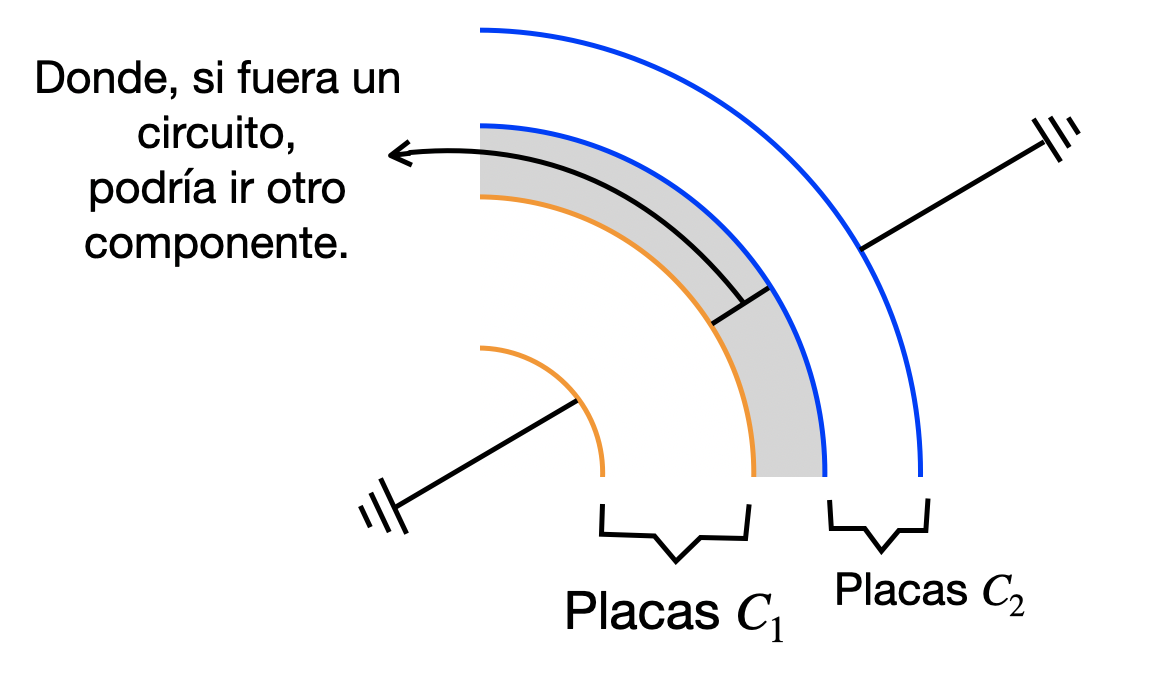
\includegraphics[width=0.5\textwidth]{Electroestática/conductores/P3IG.png}
    \end{figure}
    
    En la figura anterior el conductor de radio $a$ es el inferior izquierdo, el conductor de radio $2a$ está representado por el conductor 'con anchura' de color gris, y el conductor de radio $3a$ es el superior derecho. Las conexiones con 3 líneas representan conexiones a tierra. Y los condensadores son representados el primero con color amarillo-naranjo y el segundo con color azul. 
    
    \medbreak
    \item El sistema está compuesto por 3 conductores y 2 condensadores, como las capas interna y externa tienen potencial nulo, la energía queda dada sólo por la capa intermedia

    \[U_e = \frac{1}{2}V_2(2a) = \frac{1}{8}\frac{Q^2}{8\pi\epsilon_o a}\]
    
    Esto es equivalente a calcular la capacitancia de un condensador equivalente y, haciendo uso de $V(2a)$, obtener la energía potencial con
    $U_e = \frac{1}{2}C\Delta V^2$. 

\end{enumerate}
\bigbreak
\bigbreak
\sol{4}\newline
% Podriamos especificar la alineación de las placas y agregar imagen

\begin{enumerate}[label=\alph*)]
    %a
    \item Como las dimensiones laterales de las placas son mucho más grandes que $x$, se puede aproximar el campo eléctrico de una de las placas al de un plano infinito

    \[\Vec{E} = \frac{Q}{2A\epsilon_o}\hat{x}\]

    ubicando el origen en la placa de carga $Q$, el trabajo par desplazar la placa de carga $-Q$ en $\Delta x$ es

    \begin{equation}
        \begin{split}
            W_{ext} &= Q\int^{x+\Delta x}_x \Vec{E}\cdot d\Vec{r}\\
            & = Q\int^{x+\Delta x}_x\frac{Q}{2A\epsilon_o}\,dr\\
            & = \frac{Q^2}{2A\epsilon_o}\Delta x\\
        \end{split}
        \nonumber
    \end{equation}
    \medbreak
%b
    \item Por teorema de trabajo-energía, se cumple que la diferencia de energía potencial es igual al trabajo hecho por la fuerza externa, por lo que

    \[\Delta U_e = W = \frac{Q^2}{2A\epsilon_o}\Delta x\]
    Notemos que al ser el trabajo positivo, la fuerza externa está inyectando energía al sistema, por lo que se tiene que no se conserva la energía del sistema al aumentar la separación entre las placas por un $\Delta x$
    
    La energía potencial del sistema también se puede calcular haciendo uso del condensador, donde $U_e = \frac{1}{2}Q\Delta V = \frac{Q^2}{2C}$. Como se tiene que la carga de las placas no cambia, entonces se tiene que $C$ y $\Delta V$ han de cambiar. En específico, como se separan las placas $C$ pasa a ser $\frac{\epsilon_o A}{x+\Delta x}$ (calculado en \ref{C:placas}).
%c Aux_5 Daniela Mancilla Otoño 2020
    \item Siguiendo la idea del párrafo anterior, si es que al realizar trabajo cambia la energía del sistema, lo que implica un cambio en el condensador, (carga o diferencia de potencial) entonces al mantener la batería conectada se mantendrá la diferencia de potencial igual. Con esto en mente, entonces será necesario que la carga del condensador cambie.
    
    \begin{equation}
    \begin{split}
        W_{ext} &= \int^{x+\Delta x}_x Q\Vec{E}\cdot d\Vec{r}\\
        & = \int^{x+\Delta x}_x \frac{Q^2}{2A\epsilon_o}\,dr\\
        & = \int^{x+\Delta x}_x
        \frac{(CV_o)^2}{2A\epsilon_o}\,dr\\
        & = \int^{x+\Delta x}_x
        \frac{\epsilon_o AV_o^2}{2r^2}\,dr\\
        &=\frac{\epsilon_o AV_o^2}{2}\left(
        -\frac{1}{x+\Delta x}+\frac{1}{x}\right)\\
        &=\frac{\epsilon_o AV_o^2\Delta x}{2x(x+\Delta x)}
    \end{split}
    \nonumber
    \end{equation} 
    
    \medbreak

%d
    \item La energía potencial eléctrica inicial es
    
    \[U_i = \frac{1}{2}C_iV_o^2 = \frac{\epsilon_o A}{2x}V_o^2\]
    
    la energía potencial final es
    
    \[U_f = \frac{1}{2}C_fV_o^2 = 
    \frac{\epsilon_o A}{2(x+\Delta x)}V_o^2\]
    
    de modo que
    
    \[\Delta U = U_f-U_i = -\frac{\epsilon_o AV_o^2\Delta x}{2x(x+\Delta x)}\]
    
    % Hay que mostrar que la energía que se conserva

\end{enumerate}

\bigbreak
\bigbreak

\sol{5}\newline

\begin{enumerate}[label=\alph*)]
    \item El campo eléctrico en todo el espacio puede ser obtenido haciendo uso de la Ley de Gauss y de la definición de campo eléctrico, debido a lo que será pedido en los siguientes incisos solo será calculado en el caso $\rho > a$ y $\abs{z} < L/2$. Donde se están usando coordenadas cilíndricas y el centro del cilindro como eje.\\
    
    Partamos calculando la densidad superficial de carga, la densidad de carga es superficial a causa de que estamos frente a un conductor que no puede tener campo eléctrico interno, con esto tenemos que 
    \[\sigma = \frac{Q}{2\pi aL}\]
    A causa de que está solo en el manto y el área del manto es $2\pi aL$.\\
    
    Haciendo uso de la Ley de Gauss y sabiendo que por simetría (\ref{SimetríaCilindrosInf}) hay solo campo en la dirección $\hat{\rho}$, establecemos un cilindro más grande superpuesto con el original, de radio $\rho$ y altura $h$, con esto
    %no tiene que ser infinito?, no también el largo(altura) puede ser mucha mayor al radio
    \begin{equation}
        \begin{split}
            &\oint_{Manto} \Vec{E}\cdot d\Vec{S} = \frac{Q_{enc}}{\epsilon_0}\\
            \implies &\int E(\rho)dS = \frac{\sigma 2\pi a h}{\epsilon_0}\\
            \implies &E(\rho) \int dS = \frac{\sigma 2\pi a h}{\epsilon_0}\\
            \implies &E(\rho) 2 \pi \rho h = \frac{\sigma 2\pi a h}{\epsilon_0}\\
            \implies &E(\rho) = \frac{\sigma a}{\epsilon_0 \rho}\\
            \therefore \quad &\Vec{E}(\rho) = \frac{\sigma a}{\epsilon_0 \rho}\hat{\rho}
        \end{split}
        \nonumber 
    \end{equation}
    
    \item Sea $\sigma_+$ la densidad superficial del manto del cilindro de radio $a_1$ y $\sigma_-$ la densidad superficial del manto del cilindro de radio $a_2$, tenemos que el campo eléctrico de cada cilindro será
    
    \[\Vec{E}_{a_1} = \frac{\sigma_+ a_1}{\epsilon_0 \rho}\hat{\rho}\]
    \[\Vec{E}_{a_2} = \frac{\sigma_- a_2}{\epsilon_0 \rho}\hat{\rho'}\]
    
    Si calculamos el campo en $P$ debemos sumar ambos campos, y se tiene que $\hat{\rho'} = - \hat{\rho}$, ya que están centrados en distintos ejes los campos, y en $P$ las direcciones son justo contrarias, así
    
    \[\Vec{E}_{\text{en P}} = \left( \frac{\sigma_+ a_1}{\epsilon_0 r} - \frac{\sigma_- a_2}{\epsilon_0 (d-r)} \right)\hat{\rho}\]
    
    \item Para calcular la diferencia de potencial calculamos $V(a_1) - V(d - a_2)$ por definición,
    
    \begin{equation}
        \begin{split}
            V(a_1) - V(d - a_2) &= -\int_{d-a_2}^{a_1}\left[ \frac{\sigma_+ a_1}{\epsilon_0 r} - \frac{\sigma_- a_2}{\epsilon_0 (d-r)} \right]dr\\
            &= -\left.\left[ \frac{\sigma_+ a_1}{\epsilon_0}\ln{(r)} + \frac{\sigma_- a_2}{\epsilon_0}\ln{(d-r)} \right]\right\rvert_{d-a_2}^{a_1}\\
            &\vdots \quad\\ 
            &\approx -\left[ \frac{\sigma_+}{\epsilon_0}a_1\ln{\left( \frac{a_1}{d} \right)} - \frac{\sigma_-}{\epsilon_0}a_2\ln{\left( \frac{a_2}{d} \right)} \right]\\
            \text{Donde en } \vdots \text{ se usó que } &d-a_1 \approx d\text{ y } d-a_2 \approx d\text{, al ser }d \gg a_1\text{ y } d \gg a_2\\
        \end{split}
        \nonumber
    \end{equation}
    
    Reemplazamos $\sigma_+ = Q/(2\pi La_1)$ y $\sigma_- = -Q/(2\pi La_2)$, y nos queda
    
    \begin{equation}
        \begin{split}
            \Delta V &= -\left[ \frac{Q}{2 \pi L\epsilon_0}\ln{\left( \frac{a_1}{d} \right)} + \frac{Q}{2 \pi L\epsilon_0}\ln{\left( \frac{a_2}{d} \right)} \right]\\
            &=\frac{Q}{2 \pi L \epsilon_0}\ln{\left( \frac{d^2}{a_1a_2} \right)}\\
            &=\frac{Q}{\pi L \epsilon_0}\ln{\left( \frac{d}{\sqrt{a_1a_2}} \right)}
        \end{split}
        \nonumber
    \end{equation}
    
    Lo que nos da que la capacitancia del sistema es
    \[C_{tot} \approx \frac{Q}{\Delta V} = \frac{\pi \epsilon_0 L}{\ln{\left( \frac{d}{\sqrt{a_1a_2}} \right)}}\]
    
    \item Como se tiene que nos piden la capacitancia por unidad de largo debemos dividir la capacitancia encontrada por $L$, así
    \[C \approx \frac{\pi \epsilon_0}{\ln{\left( \frac{d}{\sqrt{a_1a_2}} \right)}}\]
    
    \item Está situación es similar a la presentada en el problema 7.2, por lo que las cargas se distribuirían a través de los cilindros dependiendo de las razones entre sus radios, y el potencial se volvería el mismo para ambos.
    
\end{enumerate}

\sol{6}\newline

\begin{enumerate}[label=\alph*)]
    \item Digamos que la capa del radio interno tiene una carga $-Q$ en su cara exterior, y la capa externa una carga $Q$ en su cara interior. Así queda la configuración como en la siguiente imagen
    \begin{figure}[H]
        \centering
        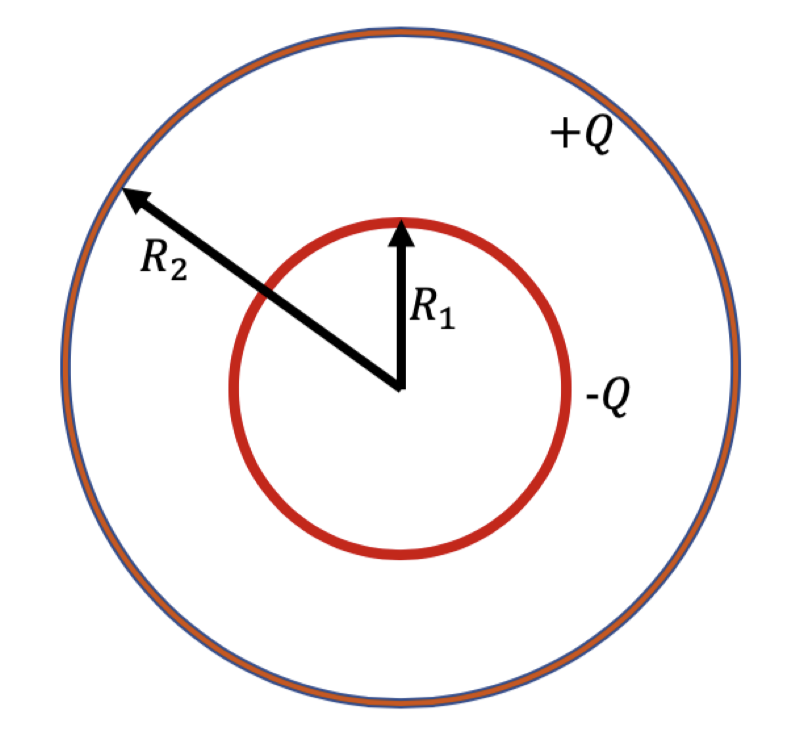
\includegraphics[width=0.47\textwidth]{Electroestática/conductores/P6IA.png}
        \label{fig:sol_6_conduc}
    \end{figure}
    
    Para calcular la capacitancia calculemos la diferencia de potencial entre ambas caras, para esto calculemos el campo eléctrico e integramos de $R_1$ a $R_2$.\\
    
    Usando Ley de Gauss y una superficie Gaussiana de largo $L$ y radio $\rho$, con $R_1 < \rho < R_2$,
    \[\oint_{Manto} \Vec{E}\cdot d\Vec{S} = \frac{Q_{enc}}{\epsilon_0}\]
    \[\implies E(\rho) = \frac{-Q}{2 \pi L \epsilon_0 \rho}\]
    Ahora calculamos la diferencia de potencial,
    \[\Delta V = V(R_2) - V(R_1) =-\int_{R_1}^{R_2}\frac{-Q}{2 \pi L \epsilon_0 \rho}d\rho = \frac{Q}{2\pi L \epsilon_0}\ln{\left( \frac{R_2}{R_1} \right)}\]
    Ahora usando $C = Q/\Delta V$ podemos obtener la capacitancia del sistema
    \[C = \frac{Q}{\Delta V} = \frac{2\pi L \epsilon_0}{\ln{\left( \frac{R_2}{R_1} \right)}}\]
    \text{ }\\     
    % Problema 2 Aux 5 D. Mancilla Otoño2020 (Pauta en Ucursos)
    
    \item \textbf{(Sin valores actualmente)} El nuevo condensador es como el mostrado a continuación
    \begin{figure}[H]
        \centering
        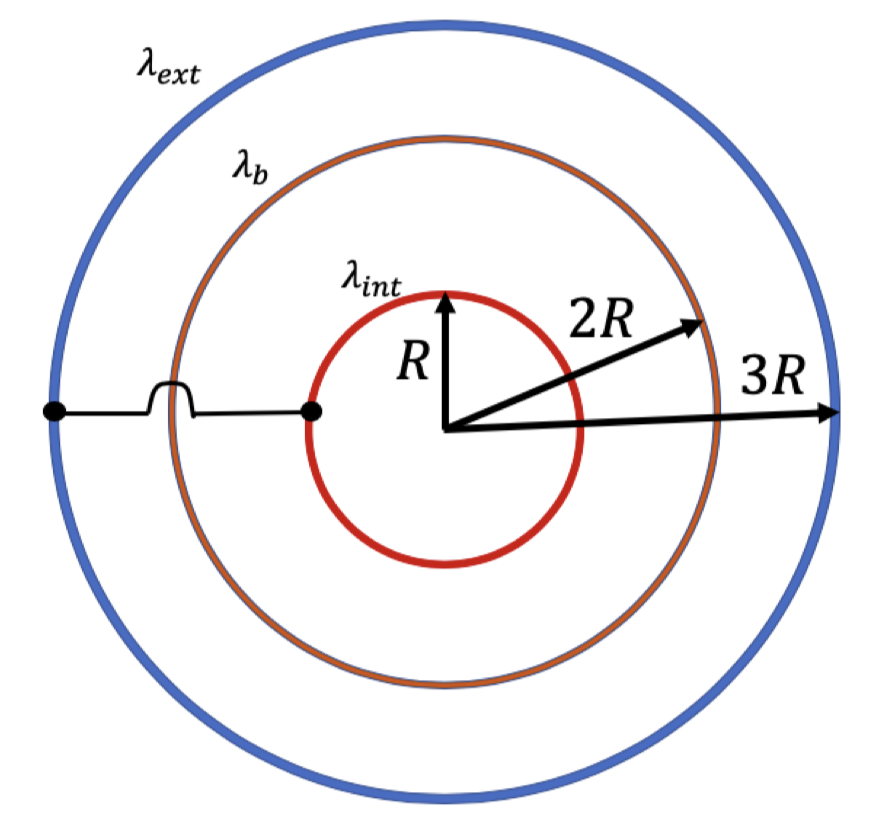
\includegraphics[width=0.47\textwidth]{Electroestática/conductores/P6IB.png}
    \end{figure}
    % Completar respuestas con desarrollo y resultados
    Como se tiene que la capa de radio $R$ y la de radio $3R$ están conectadas entonces sus potenciales son iguales, sabiendo esto y con la Ley de Gauss se puede calcular el campo eléctrico y obtener expresiones para los voltajes. Y usando $V(R) - V(2R) = V(3R) - V(2R)$ se puede despejar $\lambda_{int}$. Luego usando que son conductores y comienzan neutrales se tiene $0 = \lambda_{ext} + \lambda_{int} + \lambda_b$, y se puede obtener el valor de $\lambda_{ext}$
    % Completar respuestas con desarrollo y resultados    
    \item Para despejar la capacitancia se ocupa la relación entre energía potencial eléctrica y capacitancia, y además se despeja usando la definición que la relaciona con el voltaje.
    % (Copiado del aux)
    \item Las cargas ($\lambda_{int}, \lambda_{ext} $ y $ \lambda_b$) permanecen donde se encontraban. Con respecto a $\lambda_{nuevo}$, se distribuirá de manera uniforme en la superficie exterior ($r=3R$).
    
    
\end{enumerate}
\newpage

\end{document}
